%\documentclass[sigconf]{acmart}
\documentclass[acmtog,authorversion]{acmart}
%\documentclass[acmtog]{acmart}

\usepackage{booktabs} % For formal tables
\setcitestyle{square}

\usepackage{hyperref}

\citestyle{acmauthoryear}

\newcommand{\M}{\mathcal{M}}
\newcommand{\N}{\mathcal{N}}
\newcommand{\FM}{\mathcal{F}(\M,\mathbb{R})}
\newcommand{\FN}{\mathcal{F}(\N,\mathbb{R})}
\newcommand{\LM}{L^2(\M)}
\newcommand{\LN}{L^2(\N)}
\newcommand{\Cgt}{\mathbf{C_{gt}}}
\newcommand{\tCgt}{\widetilde{\mathbf{C_{gt}}}}
\newcommand{\tphi}{\widetilde{\phi}}
\newcommand{\tvarphi}{\widetilde{\varphi}}
\newcommand{\tPhi}{\widetilde{\boldsymbol{\Phi}}}
\newcommand{\tpsi}{\widetilde{\psi}}
\newcommand{\tPsi}{\widetilde{\boldsymbol{\Psi}}}
\newcommand{\talpha}{\widetilde{\alpha}}
\newcommand{\tbeta}{\widetilde{\beta}}
\newcommand{\tindex}{\tilde{i}}
\newcommand{\red}[1]{\textcolor{black}{#1}}

\DeclareMathOperator*{\argmax}{arg\,max}
\DeclareMathOperator*{\argmin}{arg\,min}


% Copyright
%\setcopyright{none}
\usepackage{color,soul}
\usepackage{amsmath}
\usepackage{amssymb}
\usepackage{mathtools}
\usepackage{algorithmic}
\usepackage{algorithm}
\usepackage[marginclue,footnote,silent,draft]{fixme}
\usepackage{cite}
\setcopyright{acmcopyright}
%\setcopyright{acmlicensed}
%\setcopyright{rightsretained}
%\setcopyright{usgov}
%\setcopyright{usgovmixed}
%\setcopyright{cagov}
%\setcopyright{cagovmixed}

\overfullrule=0pt
\usepackage[marginclue,footnote,silent,draft]{fixme}

% DOI
%\acmDOI{10.475/123_4}

% ISBN
%\acmISBN{123-4567-24-567/08/06}

%Conference
\acmConference[SIGGRAPH ASIA]{ACM SIGGRAP ASIA Conference}{2018}{} 
%\acmConference[WOODSTOCK'97]{ACM Woodstock conference}{July 1997}{El Paso, Texas USA} 
%\acmYear{1997}
%\copyrightyear{2016}

%\acmPrice{15.00}

\begin{document}
\title{Feature-Aware Basis for Localised Functional Maps}
\author{Paper ID: 391}

%\author{Ben Trovato}
%\authornote{Dr.~Trovato insisted his name be first.}
%\orcid{1234-5678-9012}
%\affiliation{%
%  \institution{Institute for Clarity in Documentation}
%  \streetaddress{P.O. Box 1212}
%  \city{Dublin} 
%  \state{Ohio} 
%  \postcode{43017-6221}
%}
%\email{trovato@corporation.com}

% The default list of authors is too long for headers}
%\renewcommand{\shortauthors}{B. Trovato et al.}
%
\begin{abstract}
This paper investigates the definition of feature-aware basis functions in the context of shape matching with the functional maps framework. To this end, we introduce a novel class of basis functions as solutions to PDEs involving the Laplace-Beltrami operator, where a set of seed points defines the initial conditions and encodes the local geometric information in the corresponding functions. The resulting basis functions are orthonormal, multi-scale, shape-aware, centred at the selected seed points, locally-supported, efficiently computable, and isometry-invariant. With respect to these basis functions, we experimentally verify the generality of the functional map framework, the importance to properly define localised, multi-scale, and shape-aware basis functions in order to improve the quality of the computed correspondences, and the benefits for different applications, such as surface mapping and shape comparison.
\end{abstract}
%
% The code below should be generated by the tool at
% http://dl.acm.org/ccs.cfm
% Please copy and paste the code instead of the example below. 
%
\begin{CCSXML}
<ccs2012>
<concept>
<concept_id>10010147.10010371.10010396.10010402</concept_id>
<concept_desc>Computing methodologies~Shape analysis</concept_desc>
<concept_significance>500</concept_significance>
</concept>
</ccs2012>
\end{CCSXML}
%
\ccsdesc[500]{Computing methodologies~Shape analysis}
%
\keywords{Functional map, shape correspondences, shape comparison, shape analysis, basis functions}
%
\maketitle
%
%\tableofcontents
%
\section{Introduction\label{sec:INTRODUCTION}}
Shape similarity and correspondence between 3D shapes are central to several applications in geometry processing and shape analysis, such as non-rigid shape matching, co-segmentation, texture and deformation transfer. To compute mappings or correspondences between 3D shapes, one of the main approaches is to formulate them as mappings between functions, through the functional map framework, rather than among points.

Even though previous work has analysed several aspects of the functional map framework, which include function preservation (e.g., attribute/descriptor preservation, landmark/part correspondences) and regularisation (e.g., commutation with operators, distance/volume preservation, conformality) constraints, the selection of the basis functions and their effects on the functional map remain mostly un-explored. 

In this context, our aim is to investigate the definition of \emph{feature-aware basis functions} for shape analysis with the functional maps framework, which was proposed in~\citep{OVSJANIKOV2012} and then significantly extended in the follow-up works (see~\citep{OVSJANIKOV2017-STAR} for an overview). One of the main advantages of this framework is that the optimisation step, which computes the optimal functional map that aligns the descriptor functions and commutes with the Laplace-Beltrami operators on the source and target shapes, can be solved efficiently using standard numerical tools. In fact, it typically reduces to solving a linear system of equations.

\paragraph*{Limitations}
While very simple and intuitive, this procedure relies strongly on, and as a result can be severely limited by, the choice of the reduced functional bases on the source and target shapes, since all subsequent computations are done in these bases. The most common choice of the reduced basis consists in taking the first~$k$ eigenfunctions of the Laplace-Beltrami operator (i.e., related to the~$k$ smaller eigenvalues), for some~$k<<n$, where~$n$ is the number of vertices of the mesh. The Laplace-Beltrami eigenfunctions have certain desirable properties, which most notably include their multi-scale nature and their invariance to isometric deformations. The former is based on the relation between the Dirichlet energy of functions and the Laplace-Beltrami operator, which implies that the first~$k$ eigenfunctions are well-adapted for representing sufficiently smooth functions on the surface. Increasing~$k$ therefore allows us to construct a basis, capable of representing higher-frequency functions, at the expense of a higher computational complexity and sensitivity to noise. Indeed, it has been shown that the Laplace-Beltrami eigenfunctions form an \emph{optimal} basis for representing sufficiently smooth functions. Moreover, the space spanned by the first~$k$ eigenfunctions can be shown to be stable to non-isometric perturbations, under certain conditions, related to the spectral gap between the~$k$'th and~$(k+1)$'st eigenvalues.

Despite these advantages, the Laplace-Beltrami eigenfunctions also have the following key limitations.
%
\begin{itemize}
\item Their stability properties depend on the spectral gap between consecutive eigenvalues, which is not always easy to control.
\item They are not well-adapted for representing localised functions, such as the Dirac~$\delta$ functions, which are required for converting a functional map to a point-to-point one.
\item They are numerically sensitive to shape discretisation and have ambiguities related to the selected number of eigenpairs, eigenvalue multiplicity, and sign changes. Furthermore, they can be computationally expensive, since evaluating them requires solving a large eigenvalue problem.
\item They are purely ``global,'' and are not aware of local information, such as feature points or landmarks that might be present on the shapes.
\end{itemize}
%
The last point is especially important, since the construction of the descriptors (e.g., wave kernel signature) in the presence of landmarks is typically done by building localised functions around the landmarks and by expressing them in terms of the selected bases. Unfortunately, since the first few Laplace-Beltrami eigenfunctions are not well-suited for representing such localised functions, expressing them in the Laplacian eigenbasis leads to a loss of information, which in turn adversely affects the final results.

In a similar way, the compressed manifold modes~\citep{BAREKAT2017,NEUMANN2014}, which are locally-supported and orthonormal, cannot center these functions at seed points and their supports cannot be easily defined, as they implicitly depend on the minimisation of an energy functional that controls the sparsity of the solution.

\paragraph*{Contribution}
 In this paper, we show that the aforementioned limitations can be overcome without sacrificing either the multi-scale nature, or the isometry invariance of the basis functions. In particular, we show that an informative, feature-aware and often more stable basis can be constructed efficiently by solving a set of sparse linear systems. Through the proposed basis functions, we experimentally verify the generality of the functional map framework, the importance to properly define localised, shape-aware basis functions in order to improve the quality of the computed correspondences, and the benefits for different applications, such as surface mapping and shape comparison.
 
The idea behind the proposed approach is to define a novel class of \emph{basis functions} as solutions to PDEs involving the Laplace-Beltrami operator. As PDEs, we consider the harmonic and diffusion equations that have been extensively applied to shape analysis but have been never used for the definition of basis functions. To this end, a set of \emph{seed points} defines the boundary and initial conditions of the underlying differential equations, and to encode the local geometric information around the seed points in the corresponding functions. These seed points can be a set of ground-truth corresponding landmarks used to initialise the functional map between the source and target shapes, a set of feature points (e.g., high-curvature points), or a set of surface samples (e.g., the Euclidean/geodesic farthest points from a source point). 

The proposed basis functions are \emph{linear independent} in order to have a unique representation of any signal defined on the input domain~$\mathcal{M}$ in terms of the selected basis functions. After their orthonormalisation, the \emph{orthonormality} of the basis functions allows the computation of these coefficients in linear time, as the \mbox{$\mathcal{L}^{2}(\mathcal{M})$} scalar product between the input signal and the basis functions. The proposed basis functions are also \emph{multi-scale} and \emph{shape-aware} in order to encode local and global shape features.

The proposed basis functions are \emph{centred} around the selected seed points in order to make them aware of local information and \emph{localised} around these landmarks (i.e., compactly-supported) in order to better encode the local shape geometry and to reduce their storage overhead. In fact, given a discrete domain~$\mathcal{M}$ with~$n$ points, the space of functions on~$\mathcal{M}$ has dimension~$n$ and its basis functions are encoded as a \mbox{$n\times n$} matrix. This matrix can be stored only if we work with compactly-supported basis functions, or if we select a subset of~$k$ basis functions, with~$k$ much smaller than~$n$.

These new functions are \emph{efficiently computable} through the solution of a small set of sparse linear systems, without  ambiguities (e.g., as it happens of the sign of the Laplacian eigenfunctions) and parameters, \emph{robust} to shape discretisation, and \emph{isometry-invariant}, in order to address applications such as shape comparison and correspondence, where we deal with a different discretisation or poses of the shape.

\paragraph*{Overview}
After discussing previous work (Sect.~\ref{sec:RELATED-WORK}), we introduce the harmonic and diffusion basis functions (Sect.~\ref{sec:SPECTRAL-BASIS}), discuss their computation and main properties (Sect.~\ref{sec:COMPUTATION}). Then (Sect.~\ref{sec:DISCUSSION}, Sect.~\ref{sec:CONCLUSION}), we show that they improve the results of the functional map on shape comparison and correspondence with respect to the Laplacian eigenfunctions.
%
\begin{figure*}[t]
\centering
\begin{tabular}{c|ccc|ccc}
Seed points
&\multicolumn{3}{c}{Input harmonic functions}
&\multicolumn{3}{c}{Orthonormal harmonic functions}\\
(a)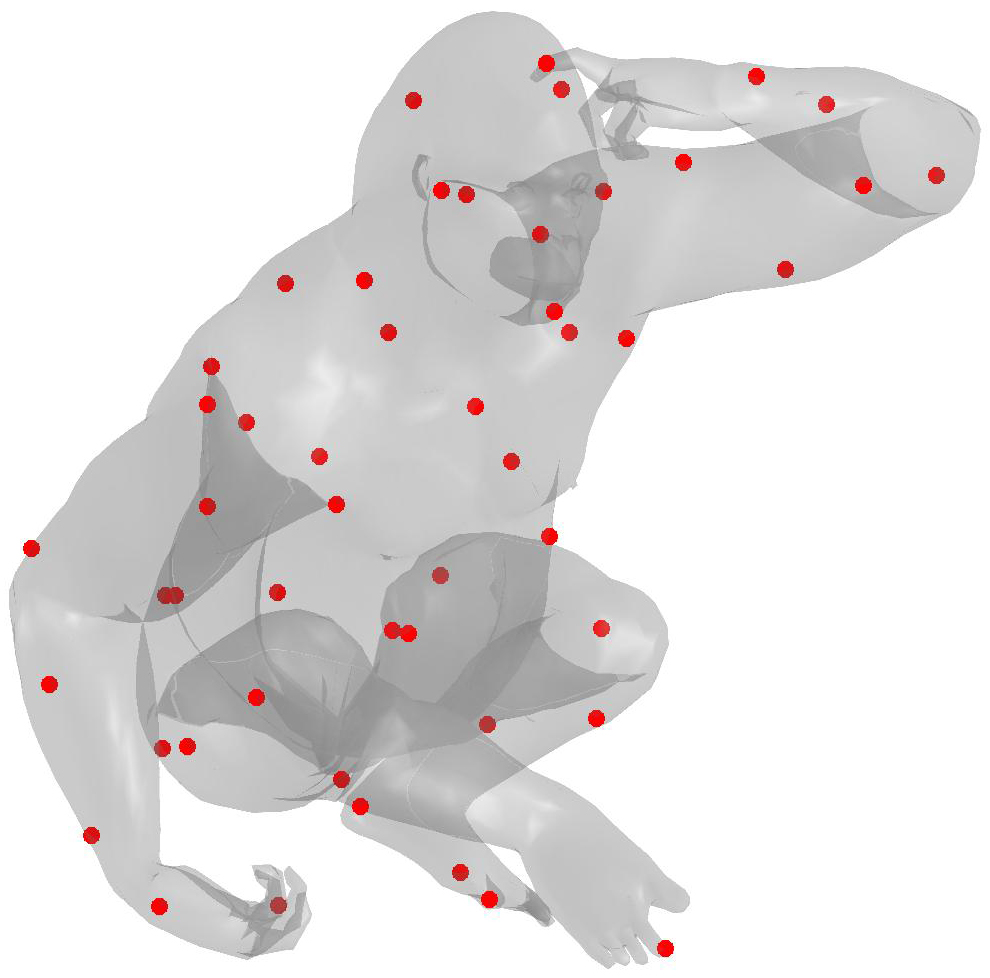
\includegraphics[height=70pt]{FMAP-images/monkey-diffusion-seed.jpg}
&(b)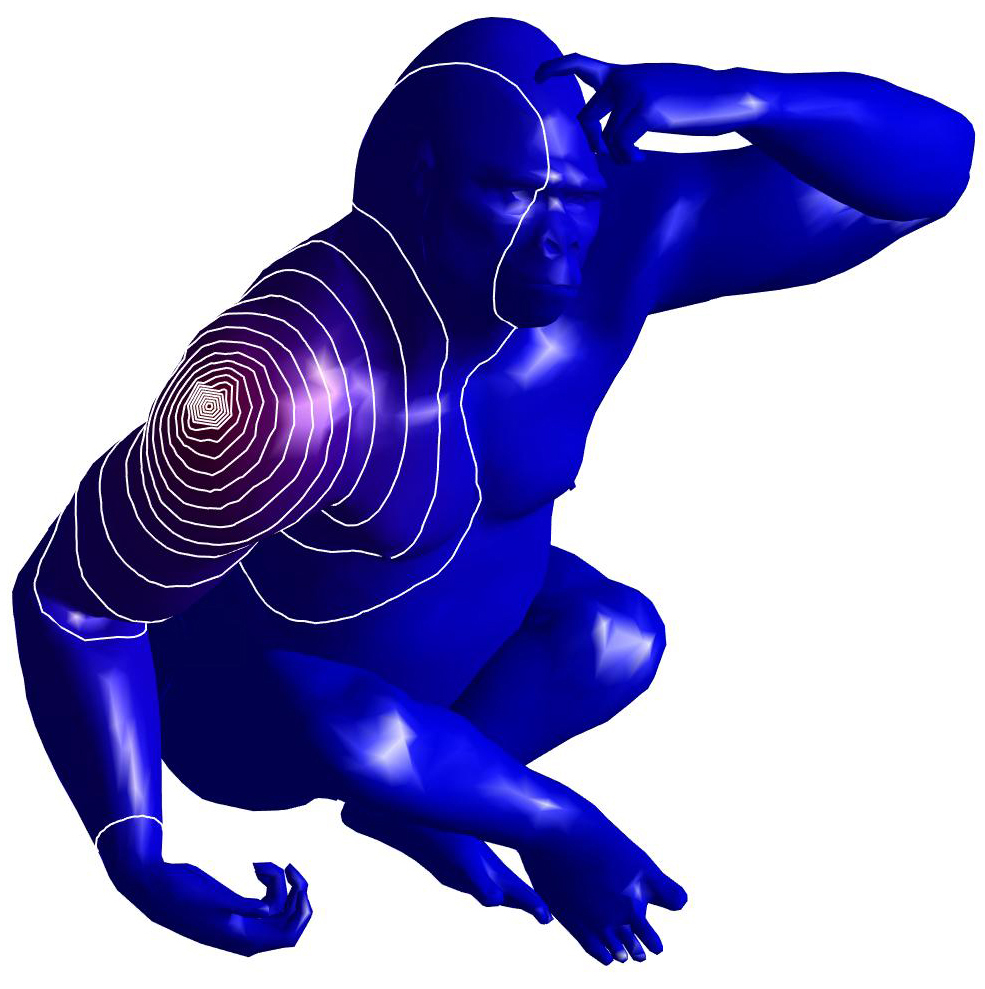
\includegraphics[height=70pt]{FMAP-images/monkey-harmonic-input-1.jpg}
&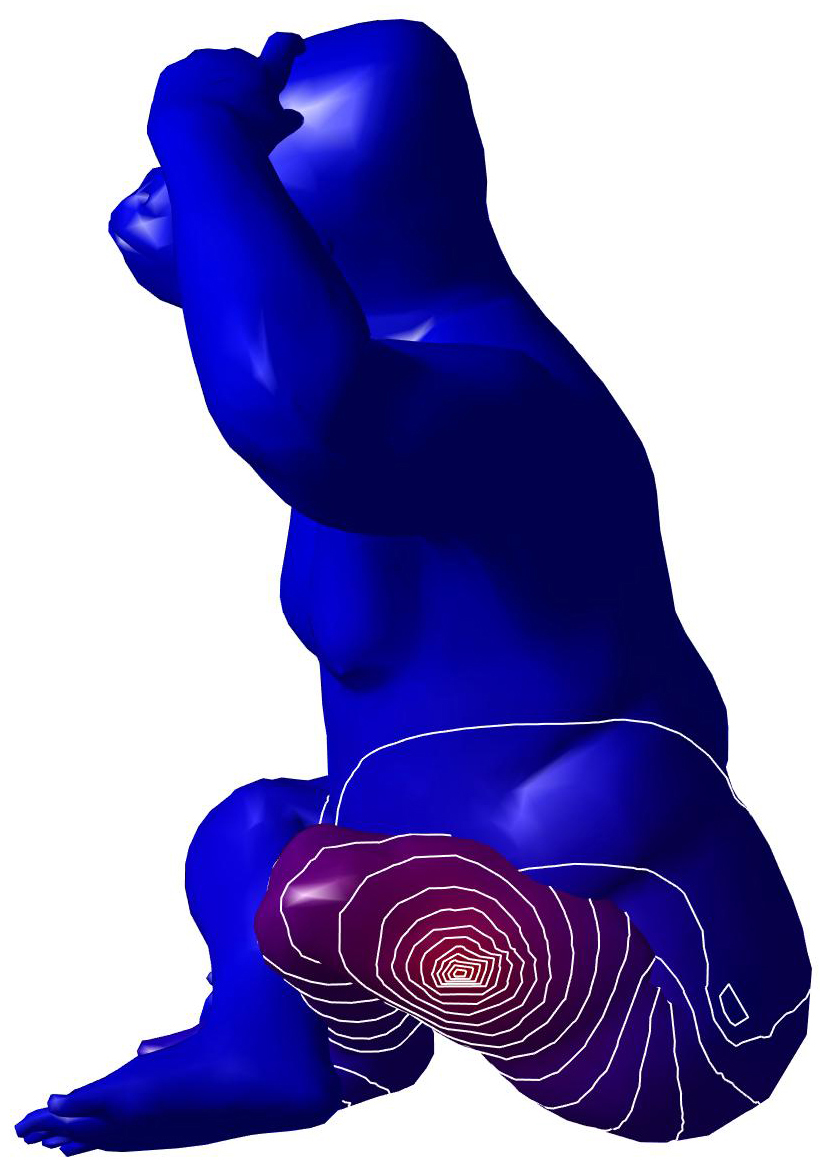
\includegraphics[height=70pt]{FMAP-images/monkey-harmonic-input-3.jpg}
&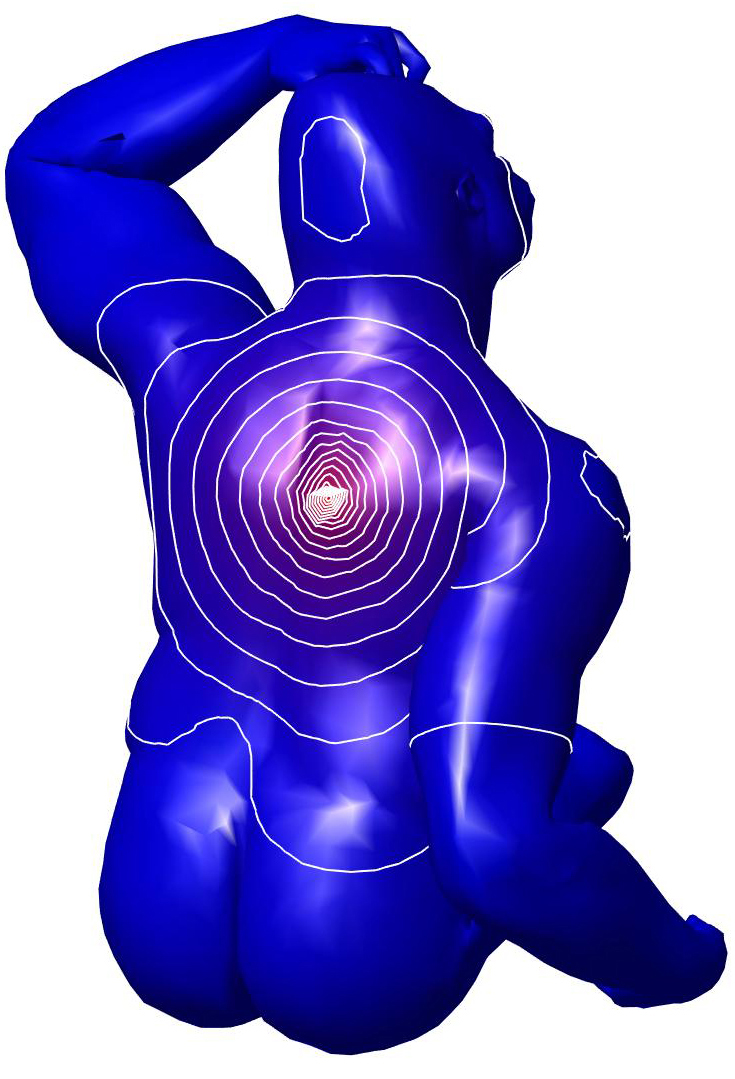
\includegraphics[height=70pt]{FMAP-images/monkey-harmonic-input-4.jpg}
&(c)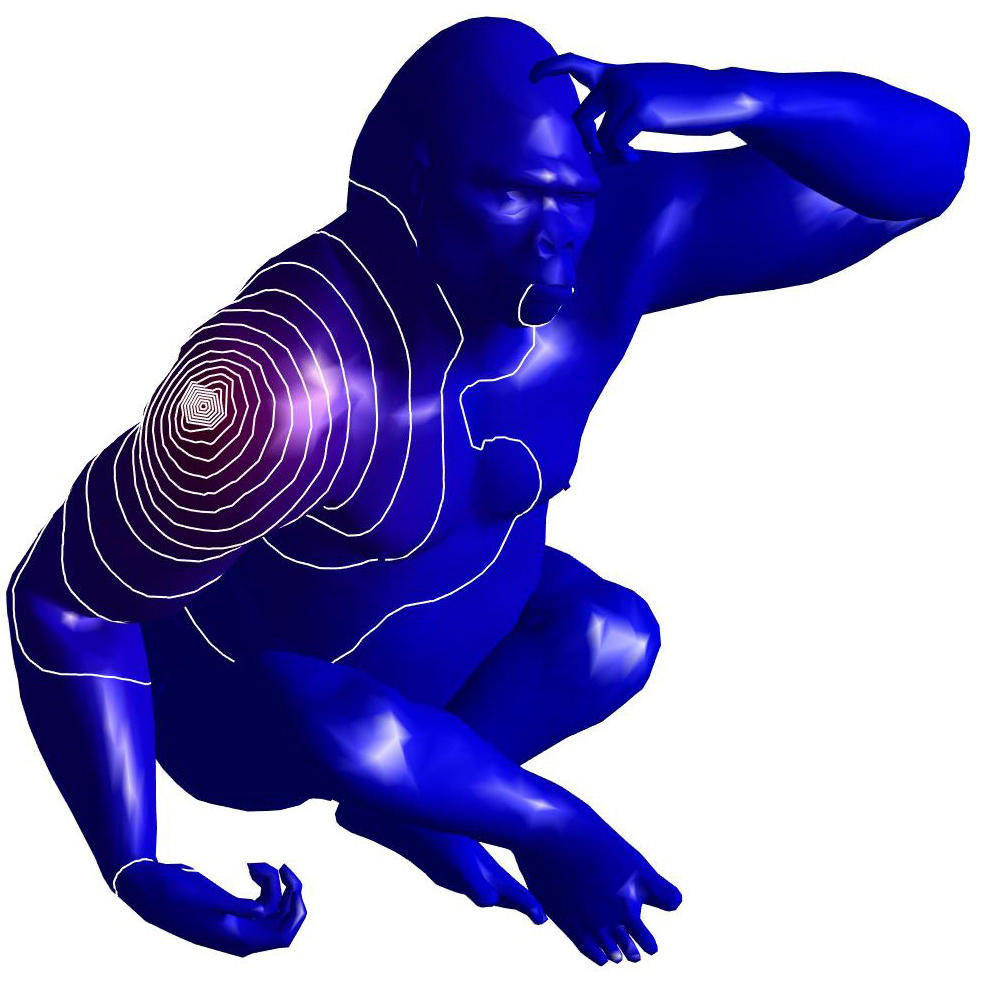
\includegraphics[height=70pt]{FMAP-images/monkey-harmonic-input-1-ORTH.jpg}
&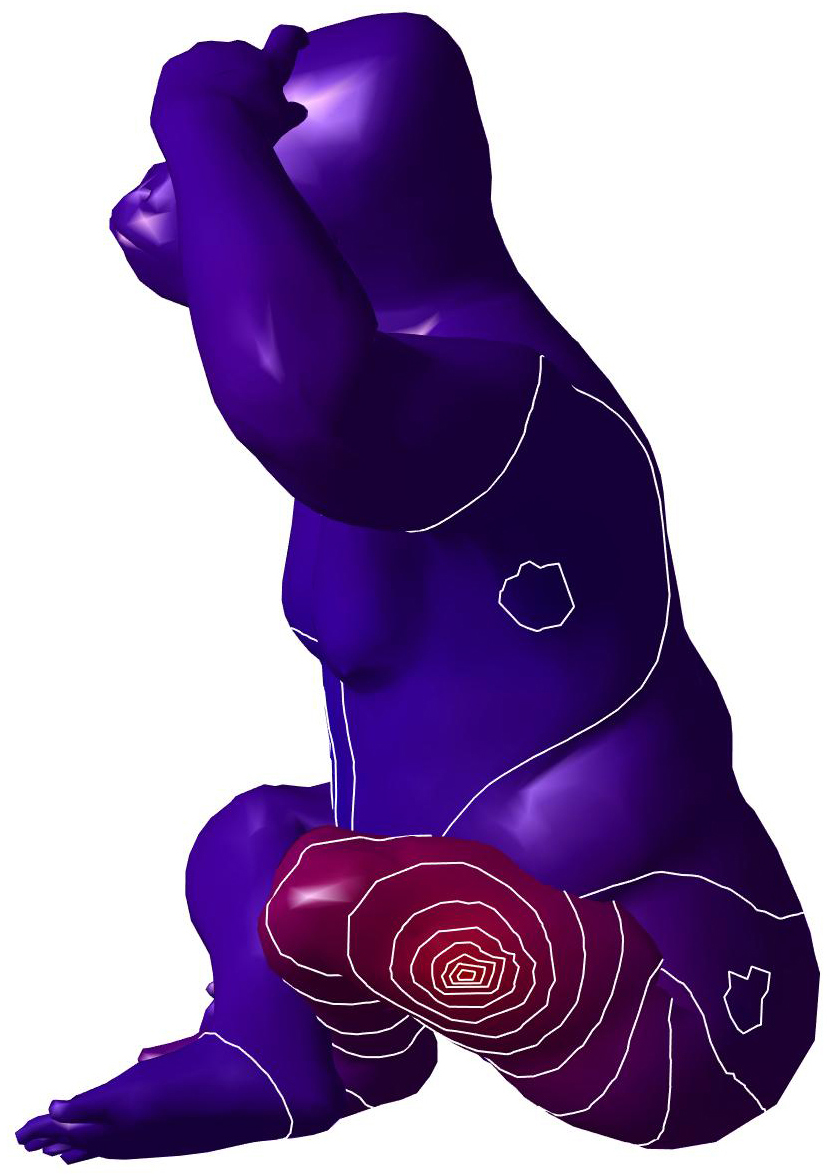
\includegraphics[height=70pt]{FMAP-images/monkey-harmonic-input-3-ORTH.jpg}
&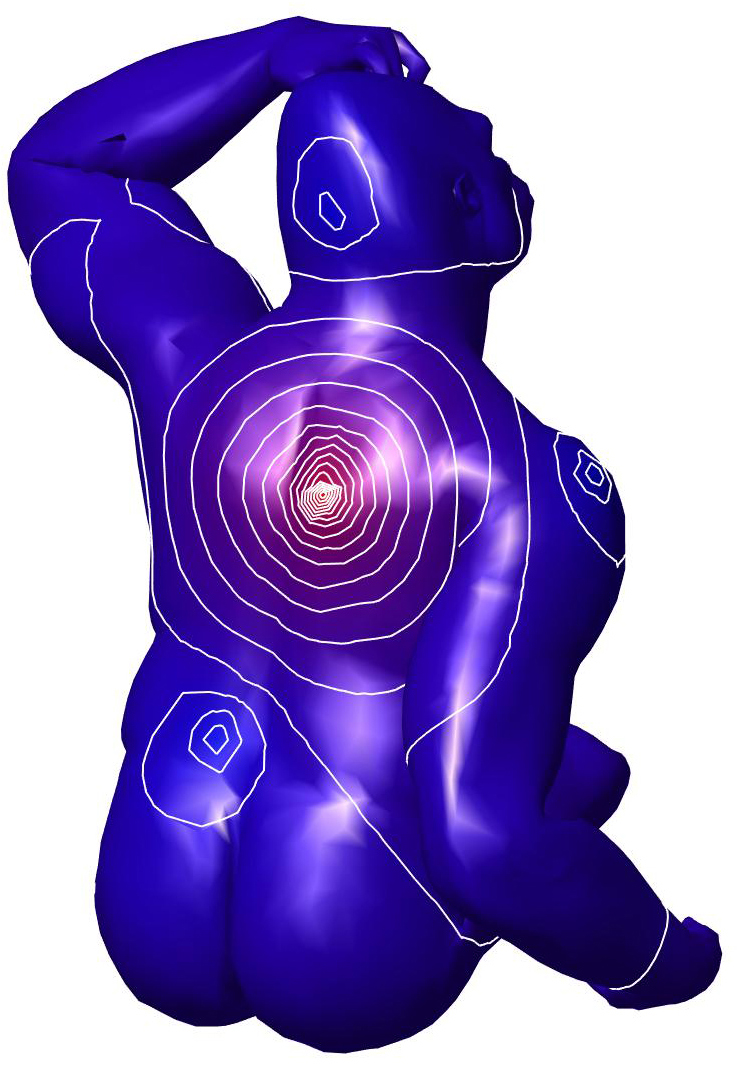
\includegraphics[height=70pt]{FMAP-images/monkey-harmonic-input-4-ORTH.jpg}
\end{tabular}
\caption{(a) Input seed points sampled uniformly on the input surface. Level-sets of the input (b) and (c) orthonormalised (second row) harmonic functions centred at 3 seed points placed on flat (spine) and rounded (harm, leg) regions of the input surface.\label{fig:MONKEY-HARM}}
\end{figure*}
%
\section{Related work\label{sec:RELATED-WORK}}
We briefly review previous work on the harmonic and heat equations, and on the functional map framework. Then, we introduce the discrete Laplacian that will be used to compute the harmonic and diffusion basis in Sect.~\ref{sec:DISCRETE-SPECTRAL-BASIS}.

\paragraph*{Harmonic equation}
Given a surface~$\mathcal{M}$, the harmonic function~$h$ is the solution of the Laplace equation \mbox{$\Delta h=0$} with Dirichlet boundary conditions \mbox{$h|_{\mathcal{S}}=h_{0}$}, \mbox{$\mathcal{S}\subset\mathcal{M}$}. Harmonic functions have been applied to the definition of shape descriptors with pairs of surface points~\citep{ZHENG2013} and coupled biharmonic bases~\citep{KONVATSKY2013}, to shape approximation~\citep{FENG2012} and deformation~\citep{JOSHI2007,JACOBSON2014,WEBER2012}.

\paragraph*{Heat equation}
Another important equation associated with the Laplace-Beltrami operator is the heat equation \mbox{$(\partial_{t}+\Delta) H(\mathbf{p},t)=0$}, \mbox{$H(\cdot,0)=h$}, where the function \mbox{$H(\mathbf{p},t)$} represents the heat distribution at the point~$\mathbf{p}$ and at time~$t$, and~$h$ is the initial distribution. The solution \mbox{$H(\mathbf{p},t)=\langle K_{t}(\mathbf{p},\cdot),h\rangle_{2}$} is written in terms of the heat kernel \mbox{$K_{t}(\mathbf{p},\mathbf{q})$}, which has been successfully applied to define multi-scale and isometry-invariant signatures and to rewrite the shape similarity problem as the comparison of two metric spaces~\citep{BRONSTEIN2009,BRONSTEIN2010-TOG,COIFMAN2006,GEBAL2009,MEMOLI2011,OVSJANKOV2010,RUSTAMOV2007,SUN2009}.

\paragraph*{Functional maps}
According to~\citep{OVSJANIKOV2012,OVSJANIKOV2017-STAR}, the functional map pipeline selects a set of ~$k_\M$,~$k_\N$ basis functions (e.g., Laplacian eigenfunctions) on the source and target shapes~$\M$ and~$\N$, respectively, and expresses~$q$ descriptor functions (e.g., wave kernel signature) on~$\mathcal{M}$ and~$\mathcal{N}$, in the corresponding bases. These expansion coefficients are stored as~$k_\M \times q$ and~$k_\N \times q$ matrices, respectively. Then, the optimal \emph{functional map} matrix~$\mathbf{C}$ of size \mbox{$k_\N \times k_\M$} is computed by aligning the descriptor functions (i.e., the expansion coefficient) and imposing their commutativity with the Laplace-Beltrami operators on the two shapes. Finally, the functional map~$\mathbf{C}$ is converted to a point-to-point map between the shapes; e.g., by mapping the Dirac~$\delta$ functions centred at each point on the source shape via the computed functional map onto the target shape, and by evaluating the nearest neighbours among the~$\delta$ functions on the target. Following the initial approach,  the  majority of works in this area use the standard Laplacian eigenbasis for functional map computation. Several extensions have been proposed including Compressed Manifold Modes
%\citep{NEUMANN2014}  
, bases derived from joint diagonalization 
%\citep{KONVATSKY2013} 
and, more recently, Localized Manifold Harmonics %\citep{melzi2017localized}. 
. None of these, however, are directly feature aware, which has also limited the utility of the functional maps framework in non-isometric shape matching.

\paragraph*{Discrete Laplacian}
The Laplace-Beltrami operator on a surface (e.g., a mesh, a points set) with~$n$ points \mbox{$\mathcal{P}:=\{\mathbf{p}_{i}\}_{i=1}^{n}$} is discretised as~ the \mbox{$n\times n$} matrix~$\mbox{$\tilde{\mathbf{L}}:=\mathbf{B}^{-1}\mathbf{L}$}$, where the \emph{mass matrix}~$\mathbf{B}$ encodes the variation of the area of the Voronoi-regions~\citep{DESBRUN1999} or triangles~\citep{reuter:cad06}, and the \emph{stiffness matrix}~$\mathbf{L}$ encodes the cotangent of the triangle angles~\citep{PINKALL1993}. An analogous discretisation applies to point sets~\citep{BELKIN2003,LIU2012} and polygonal meshes~\citep{ALEXA2011,HERHOLZ2015}. Finally, we recall that the \emph{Laplacian eigensystem} \mbox{$(\lambda_{i},\mathbf{x}_{i})_{i=1}^{n}$}, with \mbox{$\lambda_{i}\leq\lambda_{i+1}$}, satisfies the identity \mbox{$\mathbf{L}\mathbf{x}_{i}=\lambda_{i}\mathbf{B}\mathbf{x}_{i}$} and the eigenvectors are orthonormal with respect to the~$\mathbf{B}$-inner product; i.e., \mbox{$\langle\mathbf{x}_{i},\mathbf{x}_{j}\rangle_{\mathbf{B}}=\mathbf{x}_{i}^{\top}\mathbf{B}\mathbf{x}_{j}=\delta_{ij}$}.

\section{Basis functions\label{sec:SPECTRAL-BASIS}}
The idea behind the proposed approach is to define a novel class of \emph{basis functions} as solutions to PDEs involving the Laplace-Beltrami operator. More precisely, we introduce the harmonic (Sect.~\ref{sec:HARMONIC-BASIS}) and diffusion (Sect.~\ref{sec:DIFFUSION-BASIS}) basis functions, which have a~$\mathcal{C}^{2}$ smoothness, are shape-aware, isometry-invariant, and centred at a set of seed points. These points (Sect.~\ref{sec:SEED-SELECTION}) are used to define the boundary and initial conditions of the harmonic and diffusion equations and to encode the local geometric information around the seed points in the corresponding functions.

\subsection{Harmonic basis functions\label{sec:HARMONIC-BASIS}}
Given a set \mbox{$\mathcal{S}:=\{\mathbf{p}_{i}\}_{i\in\mathcal{I}}$} of seed points, we compute the \emph{harmonic basis functions} \mbox{$\mathcal{B}:=\{\psi_{i}\}_{i\in\mathcal{I}}$}, as solutions to the harmonic equation \mbox{$\Delta\psi_{i}=0$}, \mbox{$\psi_{i}(\mathbf{p}_{j})=\delta_{ij}$}, \mbox{$i,j\in\mathcal{I}$} (Fig.~\ref{fig:MONKEY-HARM}). 

\paragraph{Linear independence} 
Considering a set~$\mathcal{B}$ of harmonic functions and evaluating the relation \mbox{$\sum_{i\in\mathcal{I}}\alpha_{i}\psi_{i}=0$} at their seed points~$\mathcal{S}$, we get that \mbox{$\alpha_{i}=0$}, \mbox{$i\in\mathcal{I}$}; i.e., the harmonic basis functions centred at a set of seed points are linearly independent. 

\paragraph*{Locality}
Let \mbox{$\textrm{supp}(\psi):=\overline{\{\mathbf{p}\in\mathcal{M}:\,\psi(\mathbf{p})\neq 0\}}$} be the support of the scalar function \mbox{$\psi:\mathcal{M}\rightarrow\mathbb{R}$}. The harmonic basis functions are globally-supported and centred around the seed points; in fact, each basis function attains its maximum at the corresponding seed point (i.e., where the~$\delta$-function takes value 1), as a consequence of the maximum principle of harmonic functions.

\paragraph*{Multi-scale shape encoding}
The harmonic basis functions are not multi-scale; in fact, all the seed points are treated with the same importance in the definition of the boundary conditions.

\paragraph*{Orthogonality}
While the Laplacian eigenfunctions are orthonormal with respect to the \mbox{$\mathcal{L}^{2}(\mathcal{M})$} scalar product, the harmonic basis functions are not necessarily orthonormal. Indeed, we can orthonormalise these functions by applying the Gram-Schmidt procedure (Sect.~\ref{sec:ORTHONOTMALIZATION-PROCESS}), which has a linear computational cost in the number of basis functions. 

\subsection{Diffusion basis functions\label{sec:DIFFUSION-BASIS}}
The \emph{diffusion basis function} at~$\mathbf{p}$ is defined as the solution to the \emph{heat diffusion equation} (Fig.~\ref{fig:MONKEY-DIFFUSION})
%
\begin{equation*}
(\partial_{t}+\Delta) K_{t}(\mathbf{p},\cdot)=0,\qquad
K_{0}(\mathbf{p},\cdot)=\delta_{\mathbf{p}}\qquad (t:=0);
\end{equation*}
%
i.e., the \emph{heat kernel} \mbox{$K_{t}(\mathbf{p},\cdot)
=\sum_{n=0}^{+\infty}\exp(-\lambda_{n}t)\phi_{n}(\mathbf{p})\phi_{n}$}, represented in terms of the Laplacian eigensystem \mbox{$(\lambda_{n},\phi_{n})_{n=0}^{+\infty}$}, \mbox{$\Delta\phi_{n}=\lambda_{n}\phi_{n}$}.

\paragraph*{Linear independence}
Given a set of diffusion basis functions centred at the set~$\mathcal{S}$ of~$k$ seed points and evaluating the null relation \mbox{$\sum_{i\in\mathcal{I}}\alpha_{i}K_{t}(\mathbf{p}_{i},\cdot)=0$} at~$\mathcal{S}$, we get the homogeneous linear system \mbox{$\mathbf{K}_{t}\alpha=\mathbf{0}$}, where \mbox{$\mathbf{K}_{t}:=(K_{t}(\mathbf{p}_{i},\mathbf{p}_{j}))_{i,j\in\mathcal{I}}$} is the heat kernel matrix and \mbox{$\alpha:=(\alpha_{i})_{i\in\mathcal{I}}$} is the coefficients' array. Recalling that the heat kernel matrix is non-singular, we get that \mbox{$\alpha=\mathbf{0}$}; i.e., the diffusion basis functions are linearly independent.

\paragraph*{Locality} 
We can easily define globally- and locally-supported diffusion functions by increasing or reducing the time scale~$t$, respectively. In fact, as~$t$ becomes smaller the support of the corresponding diffusion function centred at a seed point reduces until it degenerates to the seed itself. Since the diffusion functions are compactly-supported at small scales, the coverage of the whole surface with their support depends on the selected seeds and on the support of each function. Increasing the number of seed points or the scale~$t$, all the input vertices will belong to the support of one or more functions.

\paragraph*{Multi-scale shape encoding} 
Since the diffusion basis functions encode local or global shape details for small or large values of the temporal parameter, they have a multi-scale structure.

\paragraph*{Orthogonality}
Two diffusion basis functions without overlapping supports are always orthogonal; the orthogonality of a set of diffusion basis functions with overlapping supports can be achieved with the Gram-Schmidt method at the cost of a (possibly) larger support of the orthonormal diffusion basis functions, as a matter of the linear combination of functions with a different support size during the orthonormalisation iterations. For a discussion on the support of the orthonormalised diffusion functions, we refer the reader to Sect.~\ref{sec:BASIS-DISCUSSION}.

\section{Discrete basis functions\label{sec:COMPUTATION}}
In the following, we address the computation of the harmonic and diffusion basis functions (Sect.~\ref{sec:DISCRETE-SPECTRAL-BASIS}), the selection of the corresponding seed points (Sect.~\ref{sec:SEED-SELECTION}), and their scale-invariance (Sect.~\ref{sec:ISOMETRY-INVARIANCE}). Finally, we discuss their orthonormalisation (Sect.~\ref{sec:ORTHONOTMALIZATION-PROCESS}) through the Gram-Schmidt process and the QR factorisation.

\subsection{Basis computation\label{sec:DISCRETE-SPECTRAL-BASIS}}
We now introduce the computation of the harmonic and diffusion basis functions.

\paragraph{Harmonic basis functions}
The discrete harmonic basis associated with a seed point~$\mathbf{p}_{i}$ is the solution to the linear system \mbox{$\mathbf{L}^{\star}\mathbf{g}=\mathbf{e}_{i}$}, where~$\mathbf{L}^{\star}$ is achieved by replacing the~$i$-th row of the stiffness matrix with the vector~$\mathbf{e}_{i}$, where \mbox{$\mathbf{e}_{i}^{(j)}:=\delta_{ij}$}. Harmonic functions at~$k$ seed points are efficiently computed in \mbox{$\mathcal{O}(kn)$} time with iterative solvers of sparse linear systems. Their computation is stable for the mean-value weights~\citep{FLOATER2005} while negative Voronoi-cotangent weights might induce local undulations in the resulting harmonic function (Fig.~\ref{fig:MONKEY-HARM}).
%
\begin{figure}[t]
\centering
\begin{tabular}{cc|cc}
\multicolumn{2}{c|}{Input diffusion funct.} 
&\multicolumn{2}{|c}{Orthonormal diffusion funct.}\\
\hline
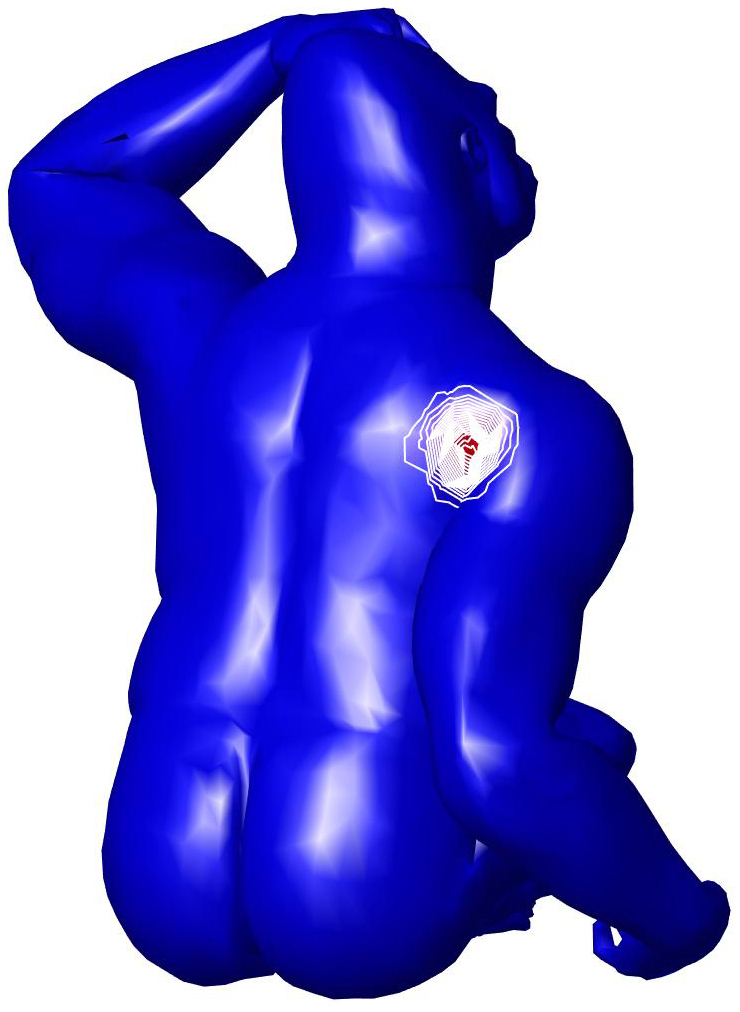
\includegraphics[height=70pt]{FMAP-images/monkey-diff-input-10-5.jpg}
&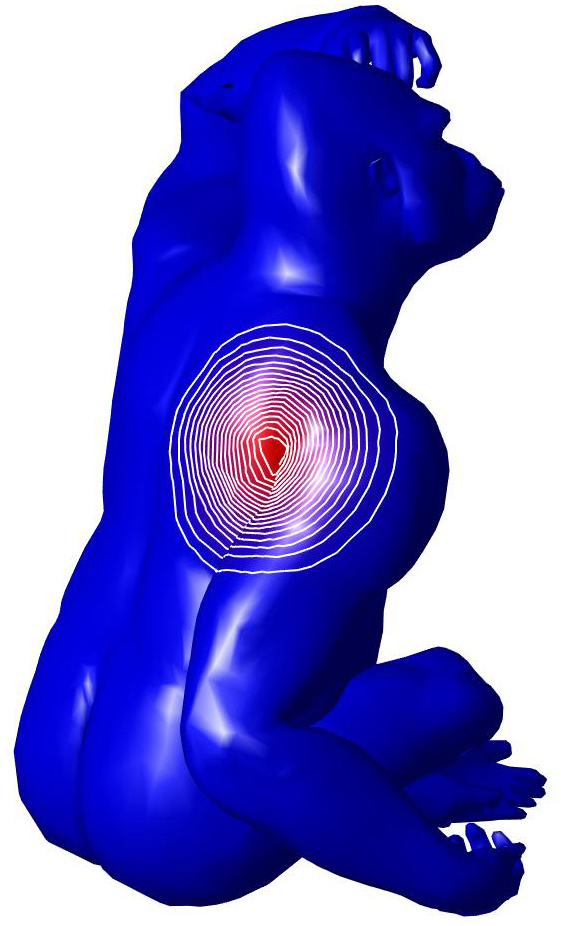
\includegraphics[height=70pt]{FMAP-images/monkey-diff-input-10-4.jpg}
&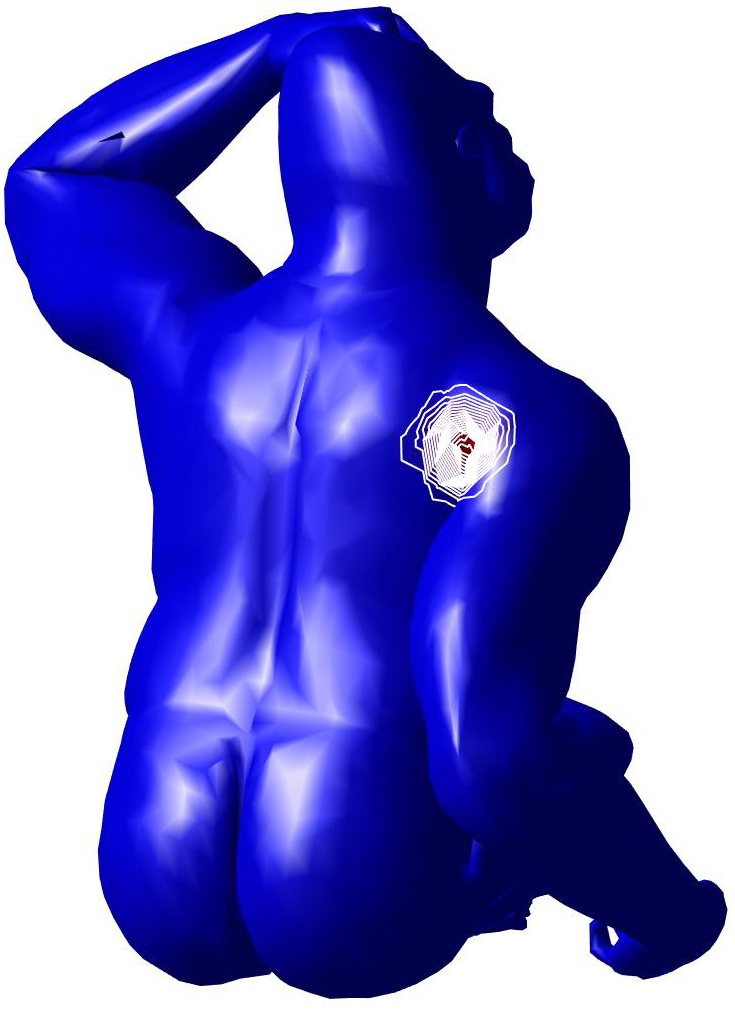
\includegraphics[height=70pt]{FMAP-images/monkey-diff-input-10-5-ORTH.jpg}
&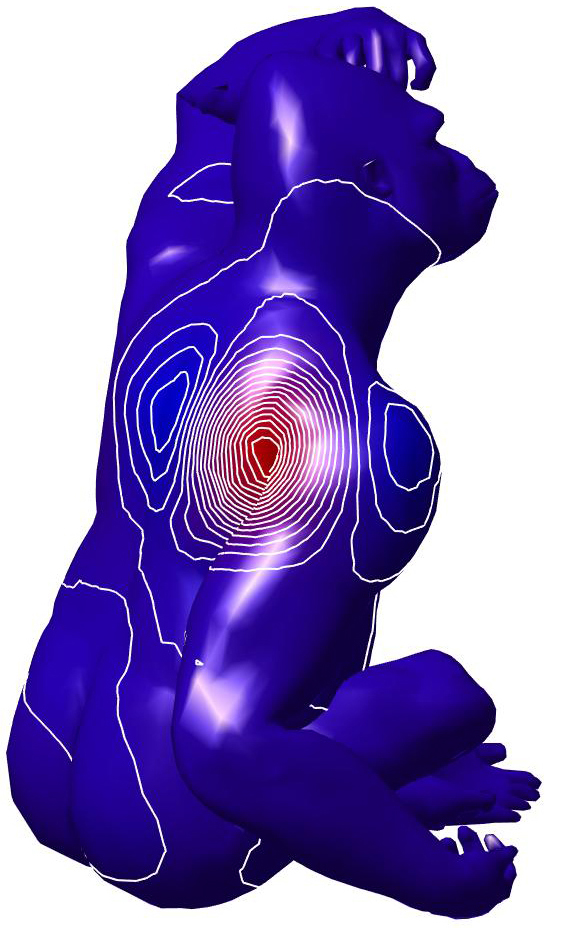
\includegraphics[height=70pt]{FMAP-images/monkey-diff-input-10-4-ORTH.jpg}\\
$t=10^{-3}$ &$t=10^{-2}$ & &\\
\hline
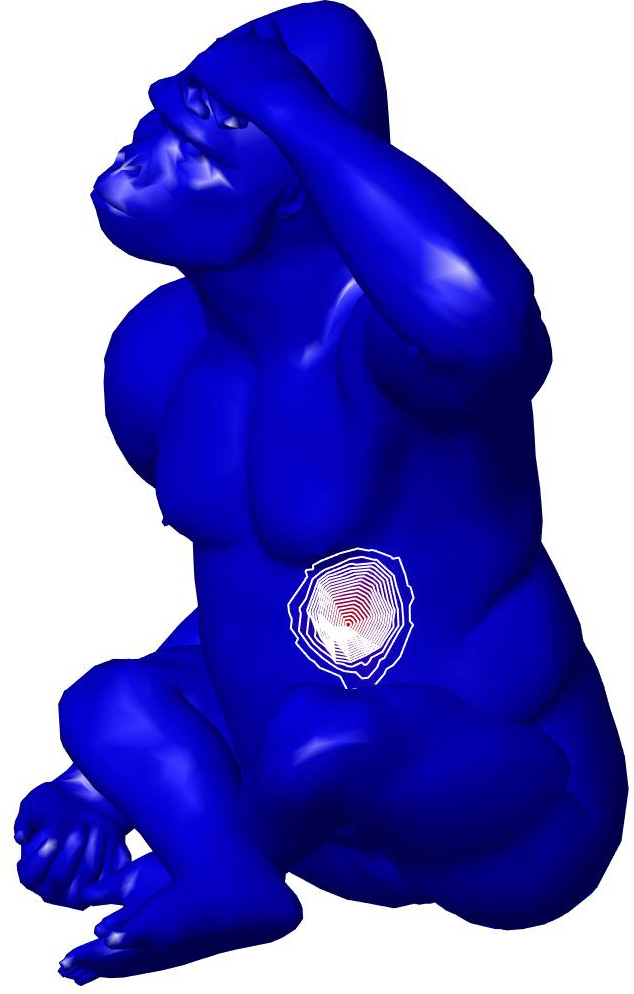
\includegraphics[height=70pt]{FMAP-images/monkey-duffusion-support-13-input.jpg}
&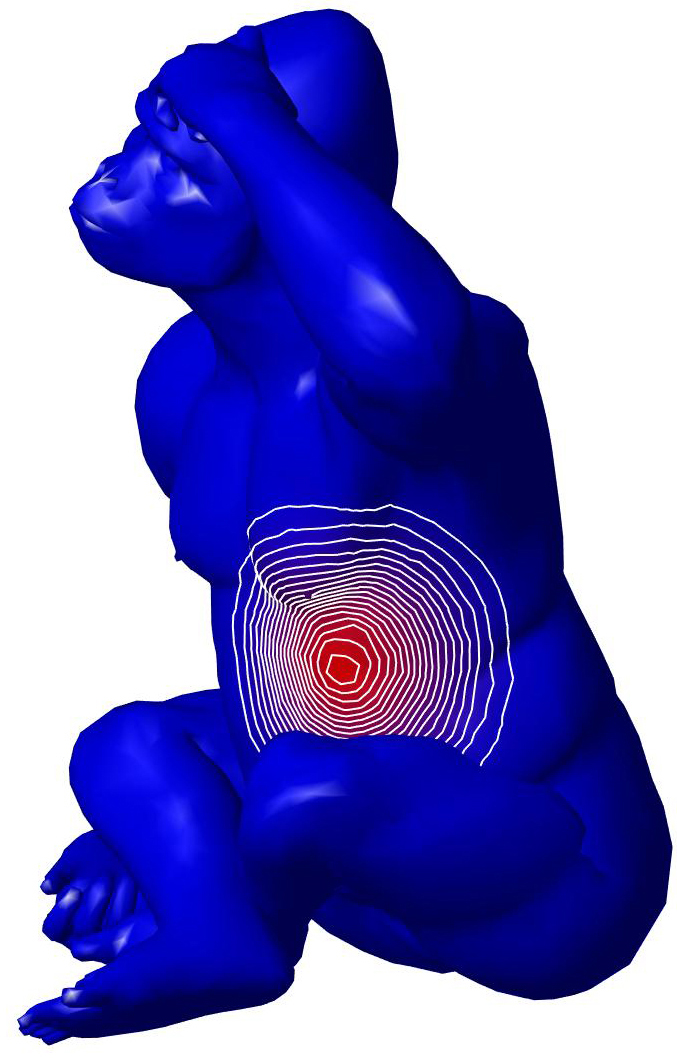
\includegraphics[height=70pt]{FMAP-images/monkey-duffusion-support-3-input.jpg}
&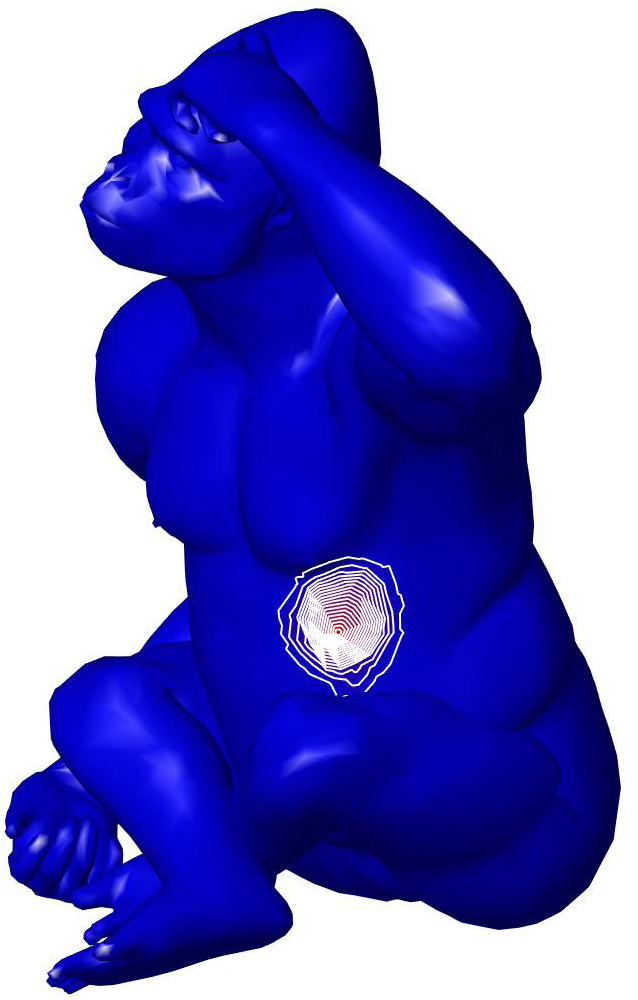
\includegraphics[height=70pt]{FMAP-images/monkey-duffusion-support-13-orth.jpg}
&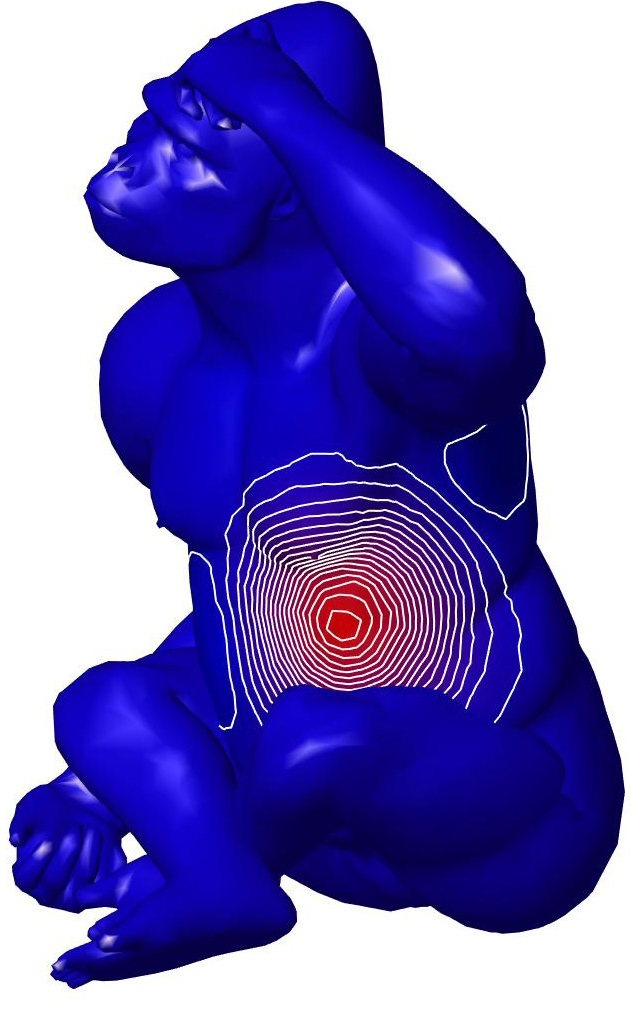
\includegraphics[height=70pt]{FMAP-images/monkey-duffusion-support-3-ORTH.jpg}\\
$t=10^{-3}$ &$t=10^{-2}$ & &\\
\hline
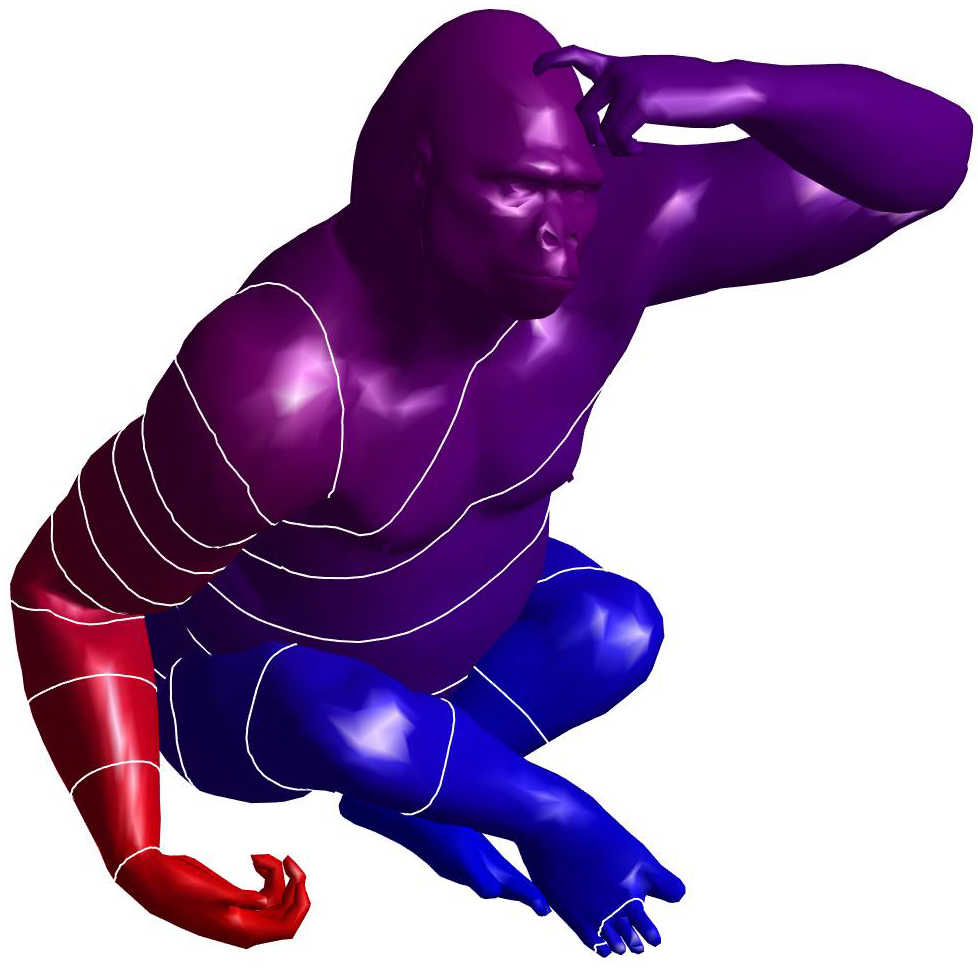
\includegraphics[height=50pt]{FMAP-images/monkey-large-scale-1-INPUT.jpg}
&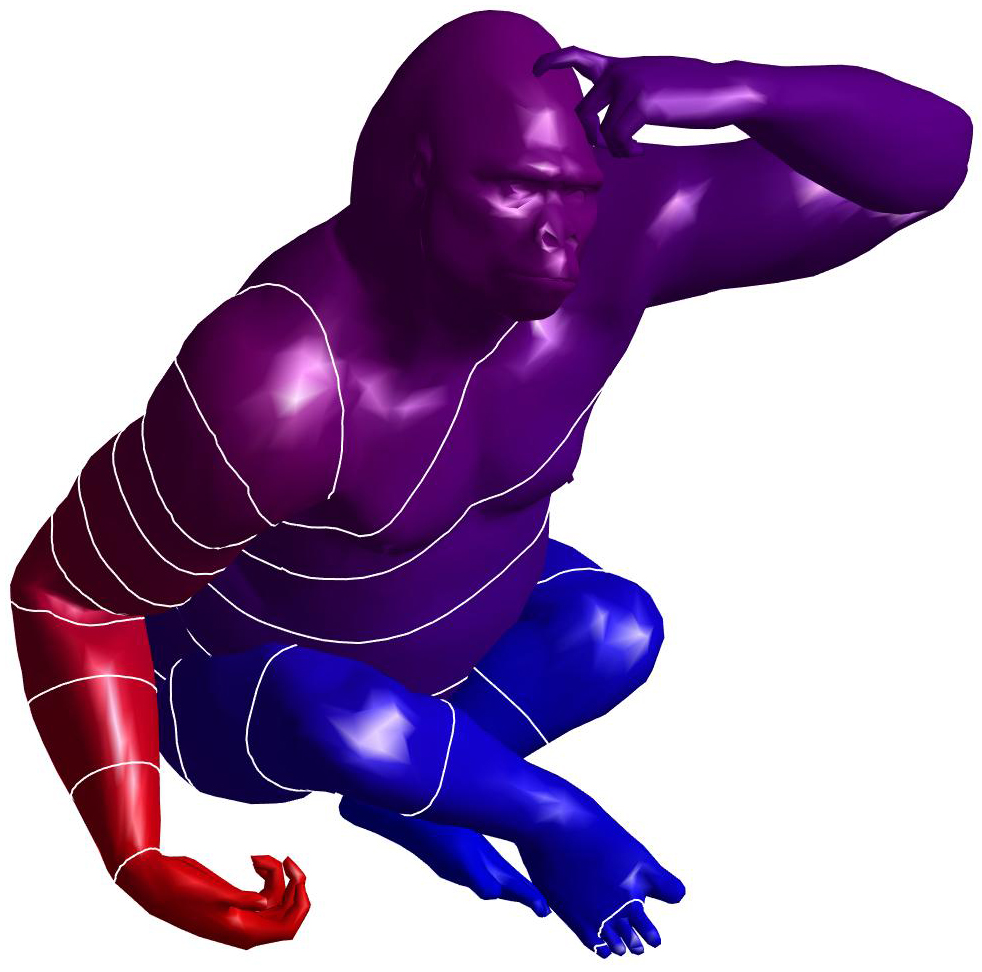
\includegraphics[height=50pt]{FMAP-images/monkey-large-scale-2-INPUT.jpg}
&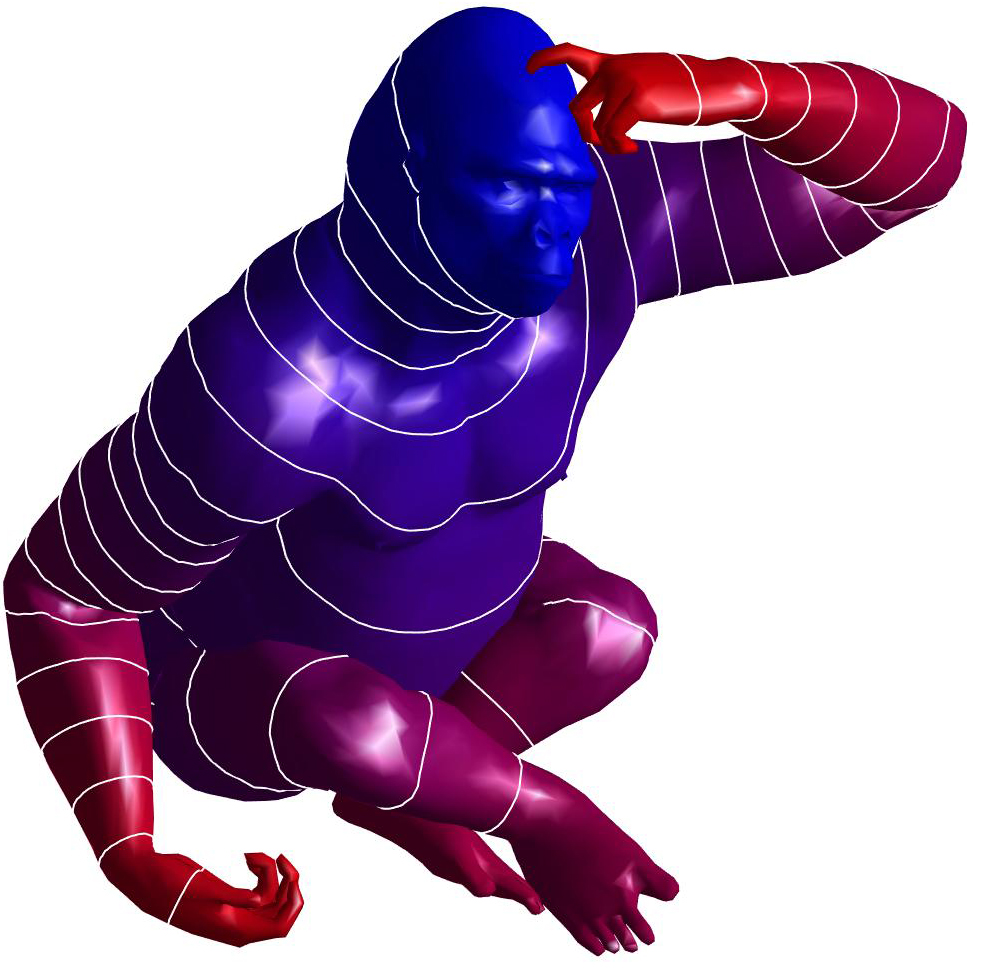
\includegraphics[height=50pt]{FMAP-images/monkey-large-scale-1-ORTH.jpg}
&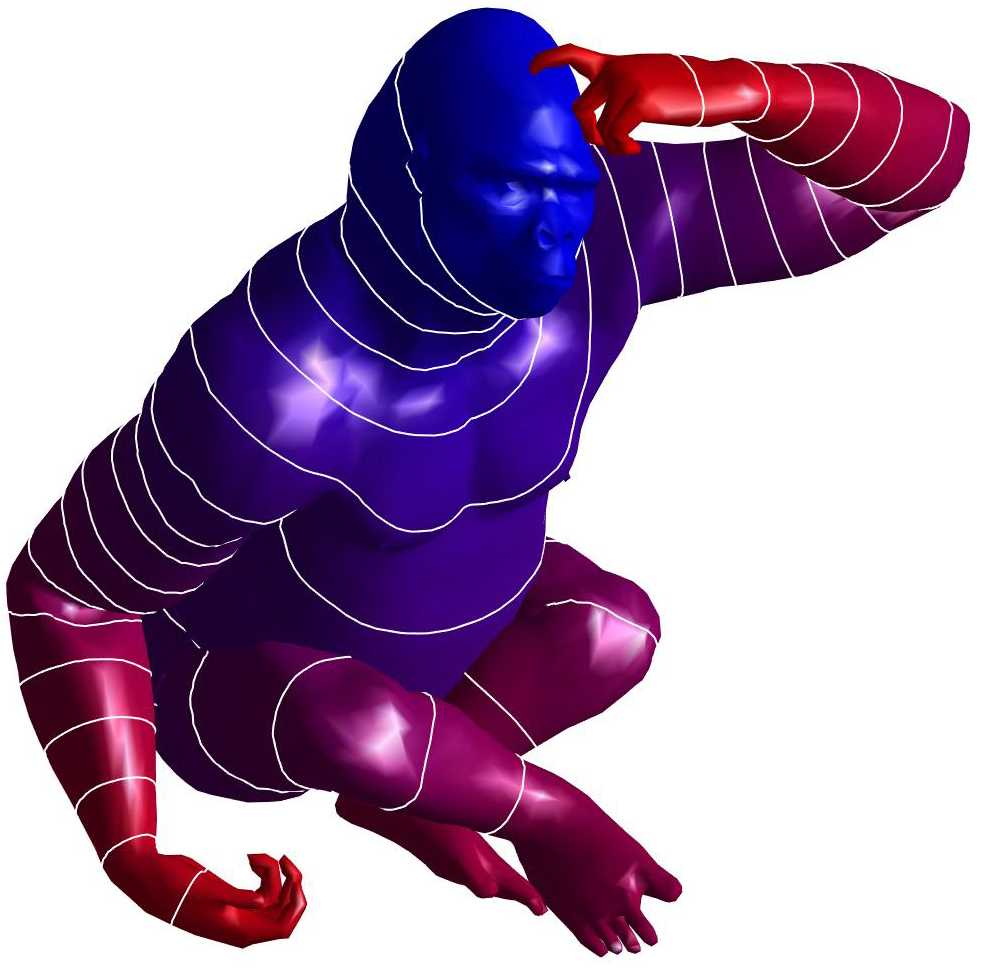
\includegraphics[height=50pt]{FMAP-images/monkey-large-scale-2-ORTH.jpg}\\
$t=0.5$ &$t=1$ & &\\
\hline
\end{tabular}
\caption{At small scales (1st, 2nd rows), the distribution of the level-sets of the input (first column) and orthonormalised (second column) diffusion functions at the same seed points have a local and multi-scale behaviour. At large scales (third row), the diffusion functions are no more centred at the seed points and have an analogous global behaviour.\label{fig:MONKEY-DIFFUSION}}
\end{figure}
%
\paragraph{Diffusion basis functions}
The diffusion basis at a seed point~$\mathbf{p}_{i}$ is represented in terms of the Laplacian spectrum as (Fig.~\ref{fig:MONKEY-DIFFUSION})
%
\begin{equation}\label{eq:EIGS-SPECTRAL-OP}
\mathbf{K}_{t}\mathbf{e}_{i}
=\sum_{i=1}^{n}\exp(-\lambda_{i}t)\langle\mathbf{f},\mathbf{e}_{i}\rangle_{\mathbf{B}}\mathbf{x}_{i}
=\mathbf{X}\mathbf{D}_{t}\mathbf{X}^{\top}\mathbf{B}\mathbf{e}_{i},
\end{equation}
%
where~$\mathbf{X}$ is the matrix whose columns are the Laplacian eigenvectors and \mbox{$\mathbf{D}_{t}:=\textrm{diag}(\exp(-t\lambda_{i}))_{i=1}^{n}$}.
%
\begin{figure}[t]
\centering
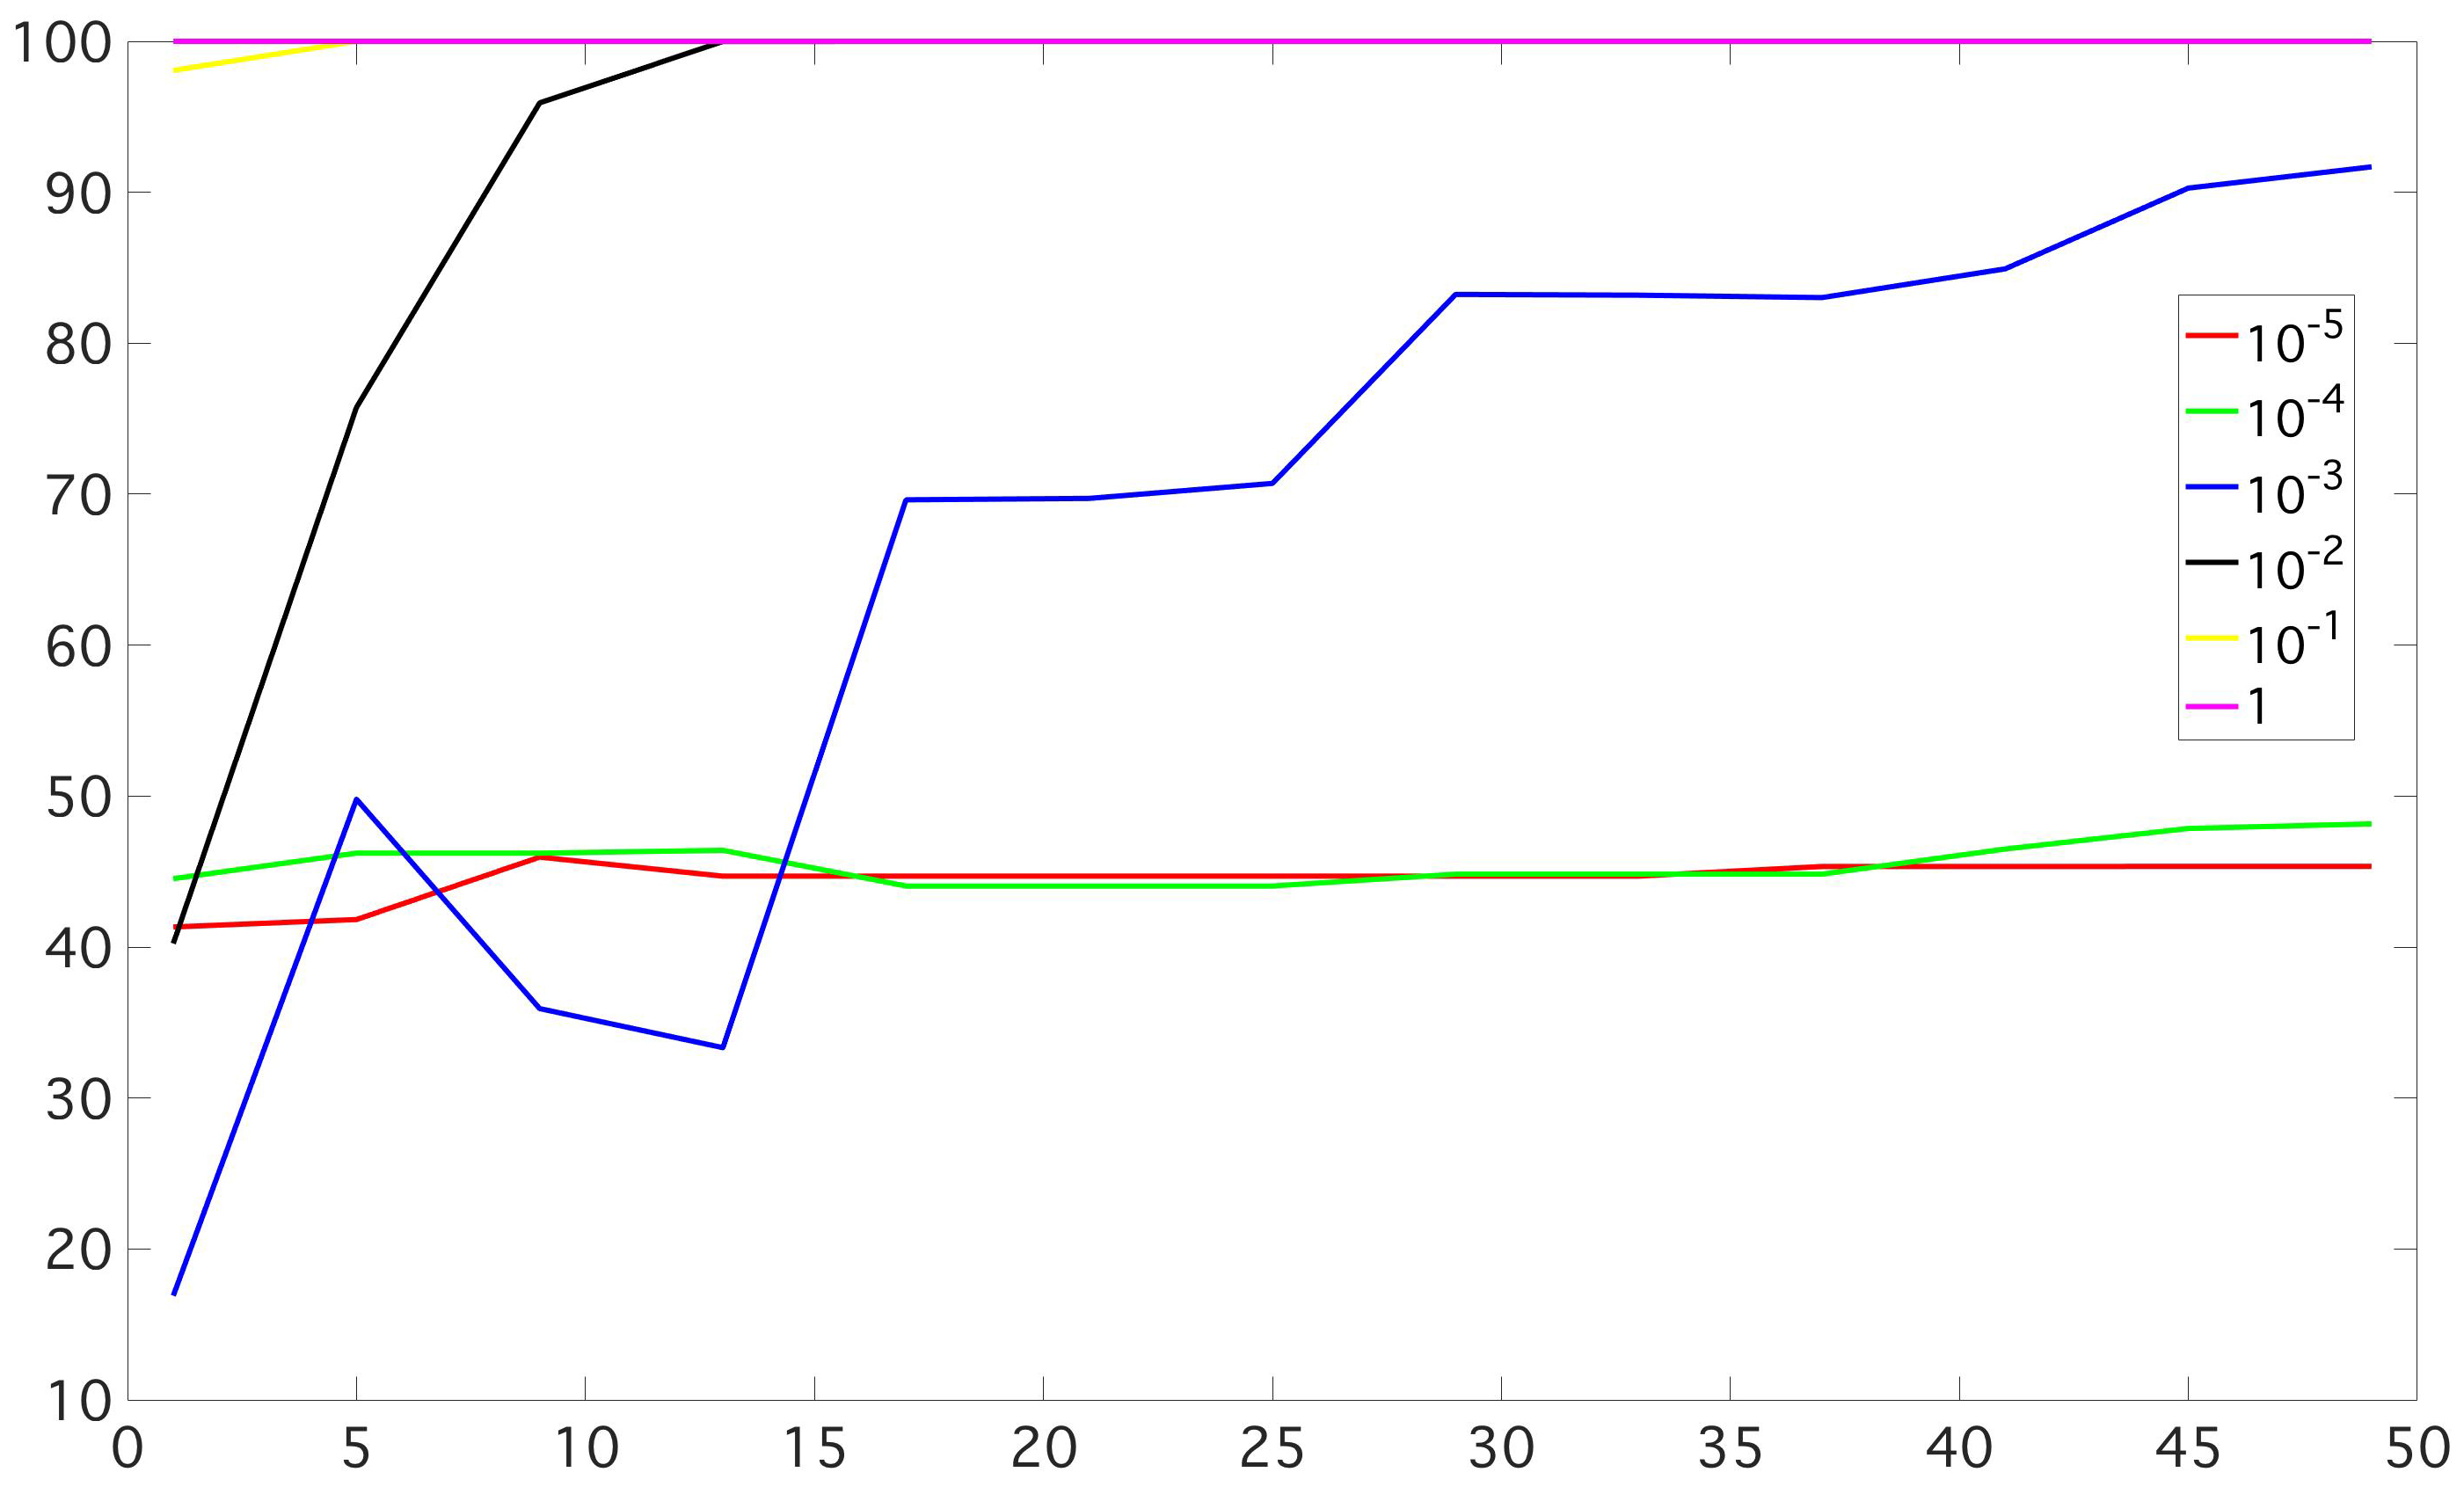
\includegraphics[height=140pt]{FMAP-images/monkey-duffusion-support-14-UPDATED-1.jpg}\\
%(b)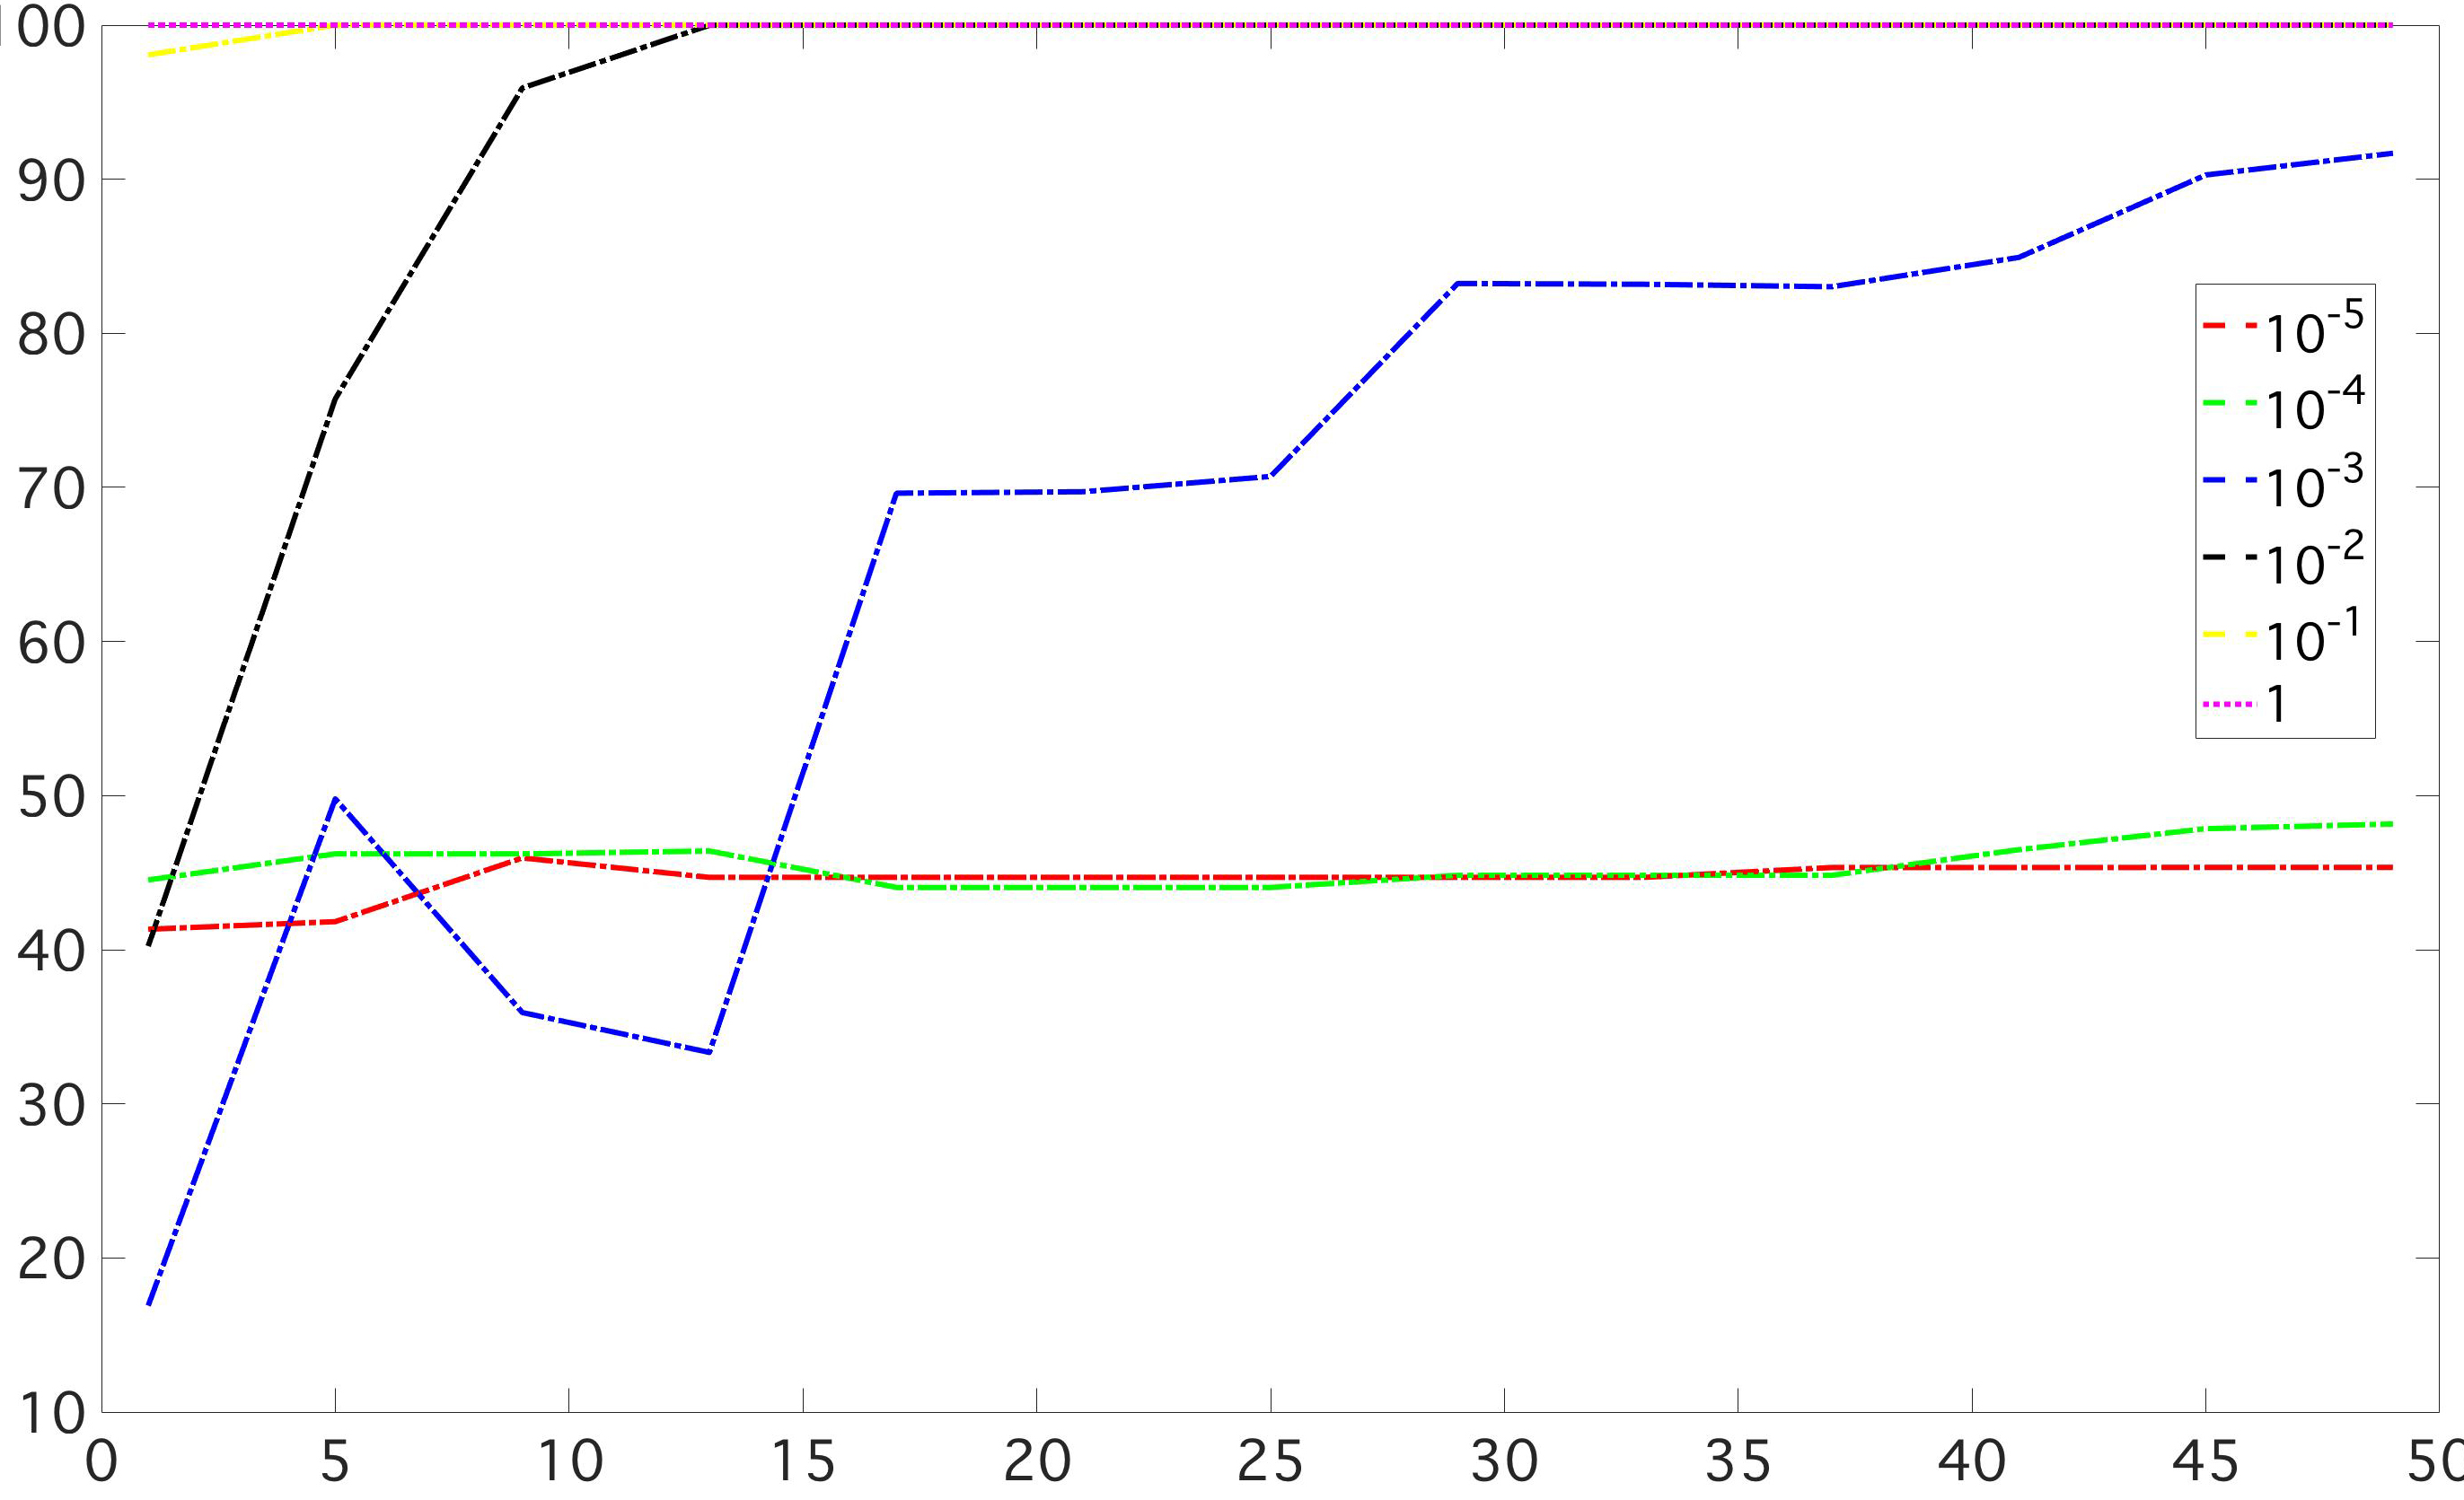
\includegraphics[height=120pt]{FMAP-images/monkey-duffusion-support-14-UPDATED-2.jpg}
\caption{Percentage ($y$-axis) of vertices belonging to the support of~$k$ input (continuous line) and orthonormal (dotted line) diffusion functions at 6 scales \mbox{$(t=10^{-i})_{i=0}^{5}$}, whose 50 seed points ($x$-axis) have been uniformly sampled on the input surface. At large scales (\mbox{$t=1$}, \mbox{$t=10^{-1}$}, respectively), the supports of a few (\mbox{$k\leq10$}) diffusion basis functions cover the whole surface. At tiny scales (\mbox{$t=10^{-5}$}, \mbox{$t=10^{-4}$}), the diffusion basis functions centred at 50 seed points have no overlapping supports. The full overlap of the continuous and dotted lines confirms that the orhonormalisation does not significantly affect the support of the multi-scale diffusion functions.\label{fig:SEEDS}}
\end{figure}

To compute this function, in Eq. (\ref{eq:EIGS-SPECTRAL-OP}) we can consider the contribution of~$s$ Laplacian eigenpairs, with~$s$ much smaller than the number of input points. Local features of the diffusion basis function, which are associated with a high frequency, are generally missing in the approximated basis function and can be recovered by considering only a high number of Laplacian eigenpairs. However, the evaluation of a large part of the Laplacian spectrum is computationally unfeasible, requires a large memory overhead, and is numerically unstable in case of duplicated or numerically close eigenvalues. In order to avoid these drawbacks and to guarantee a high approximation accuracy of the diffusion basis at small scales, we apply a multi-resolutive approximation based on prolongation operators~\citep{VAXMAN2010}, or the spectrum-free method~\citep{PATANE-CAGD2013}, which is independent of the computation of the Laplacian spectrum and has a \mbox{$\mathcal{O}(n\log n)$} cost.
%
\begin{figure*}[t]
\centering
\begin{tabular}{cc}
(a)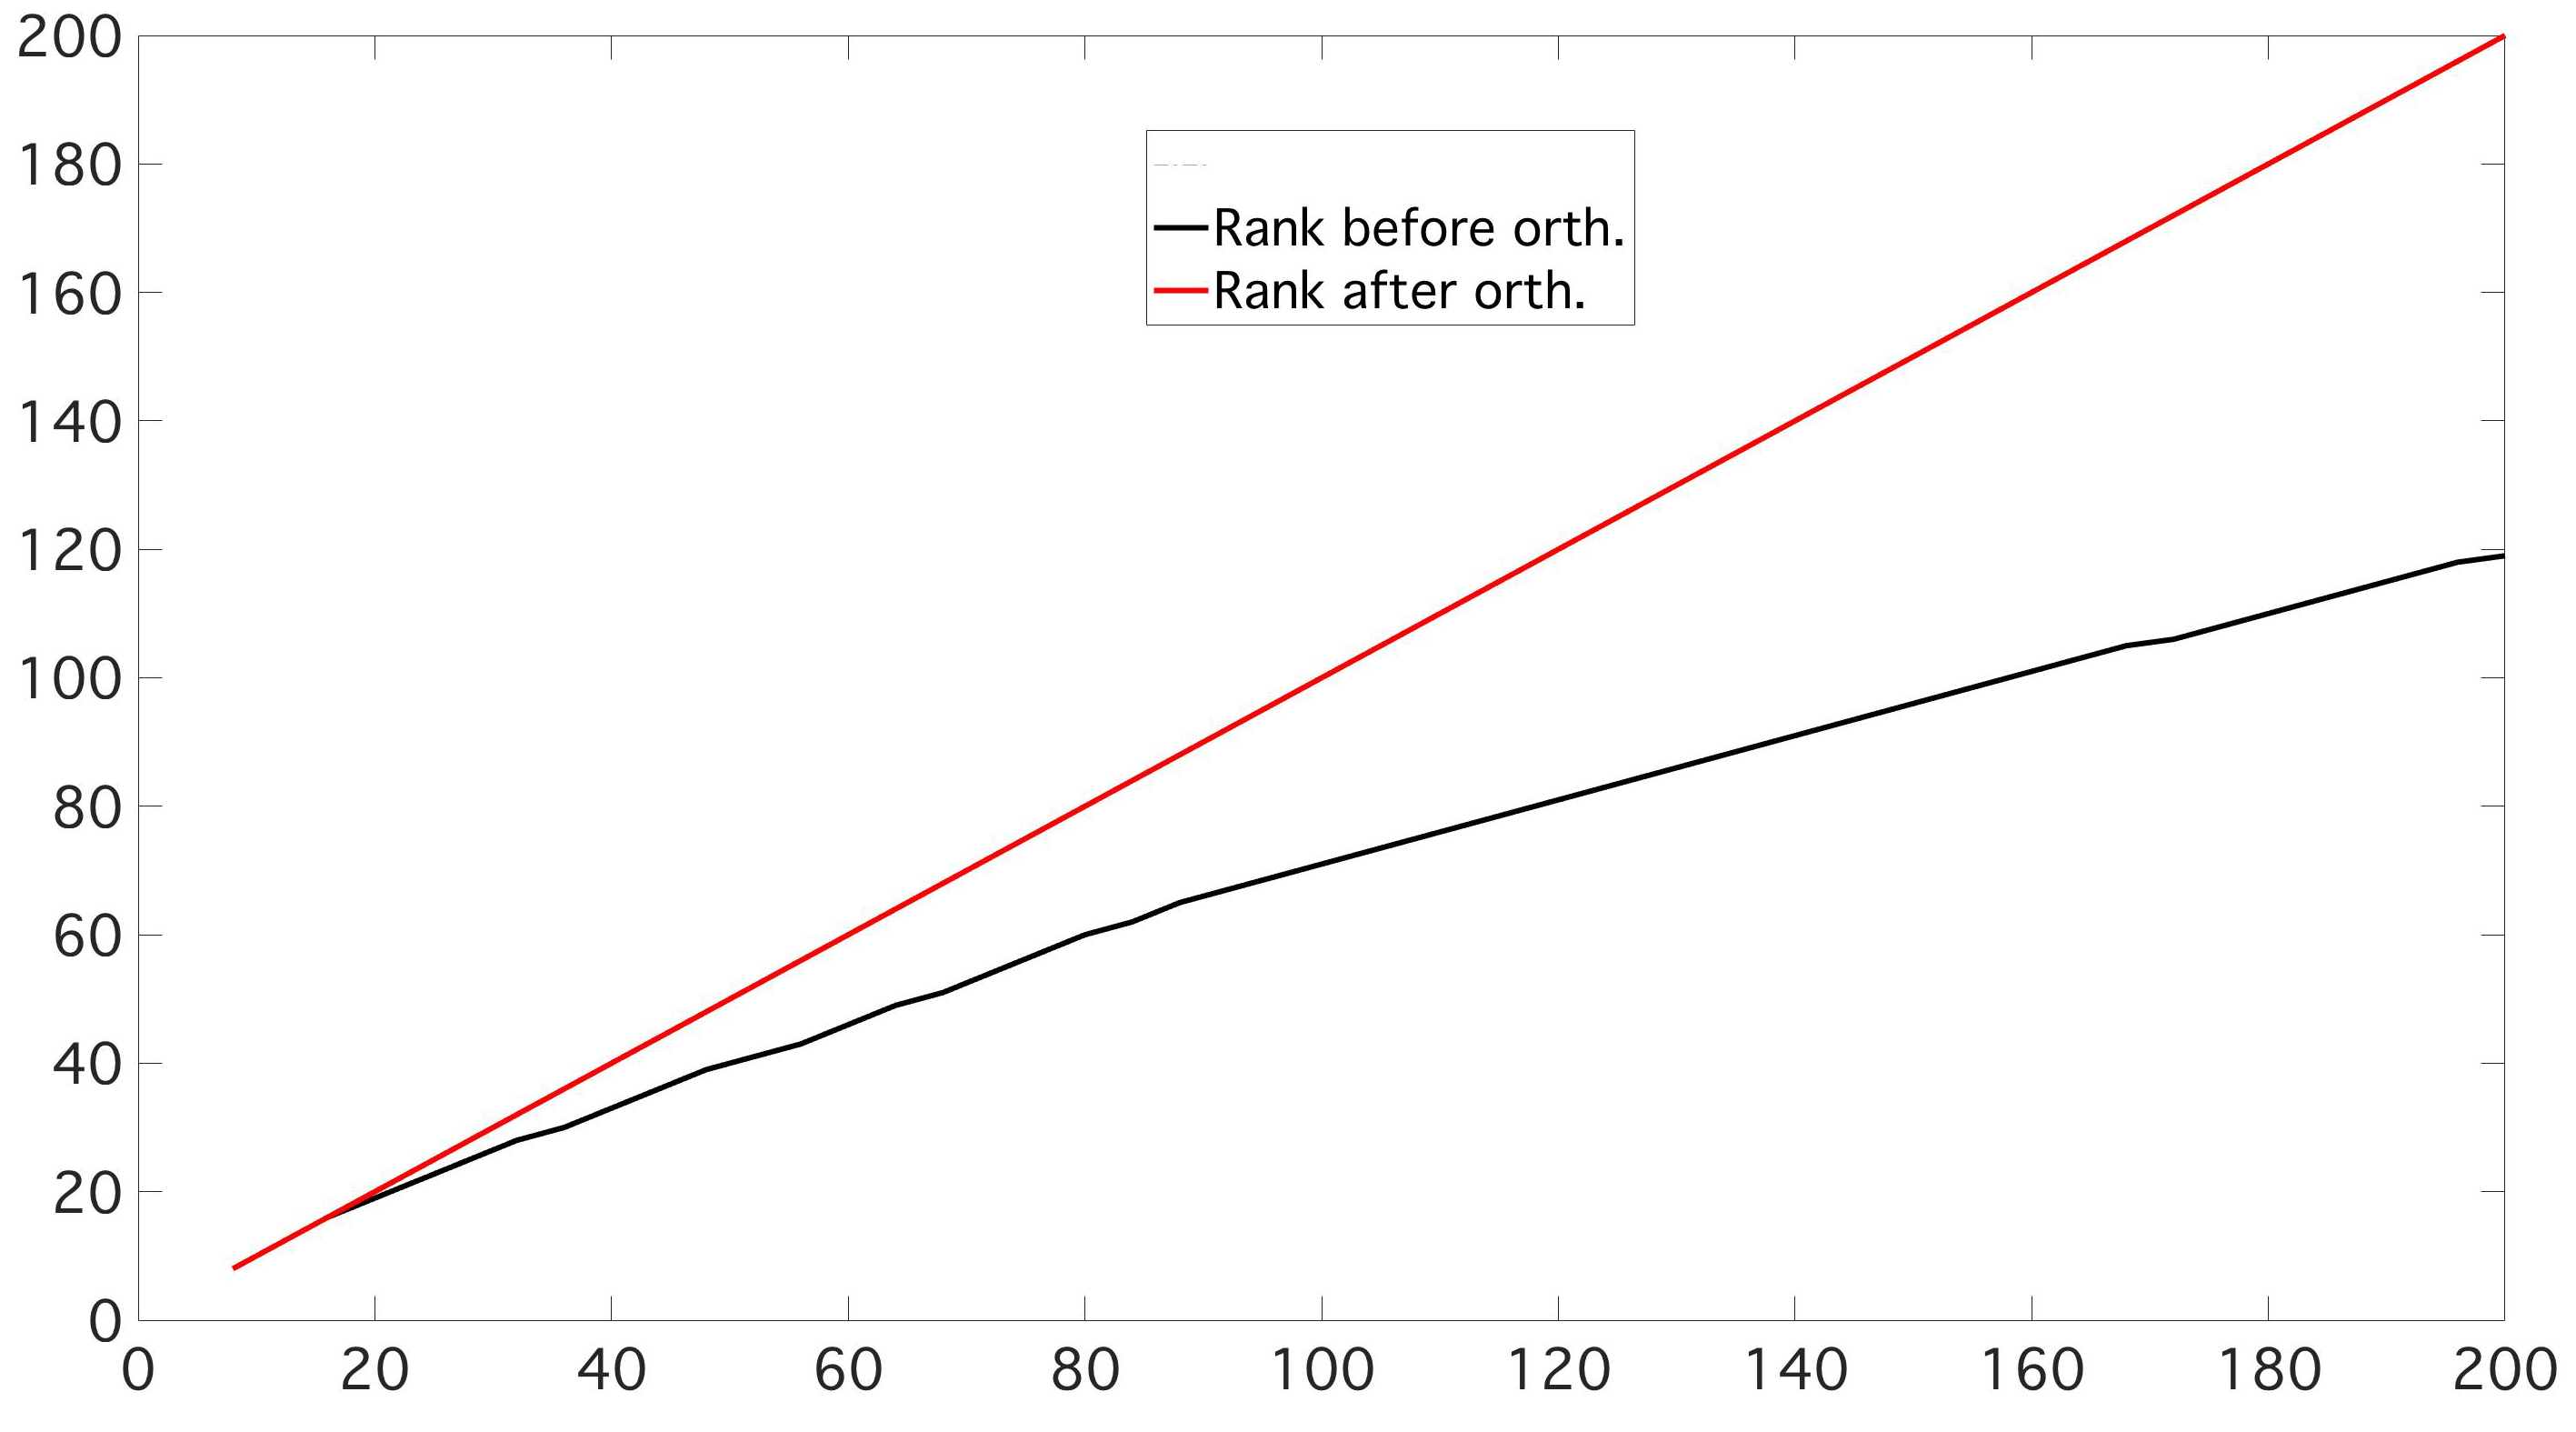
\includegraphics[width=235pt]{FMAP-images/monkey-diffusion-seed-rank.jpg}
(b)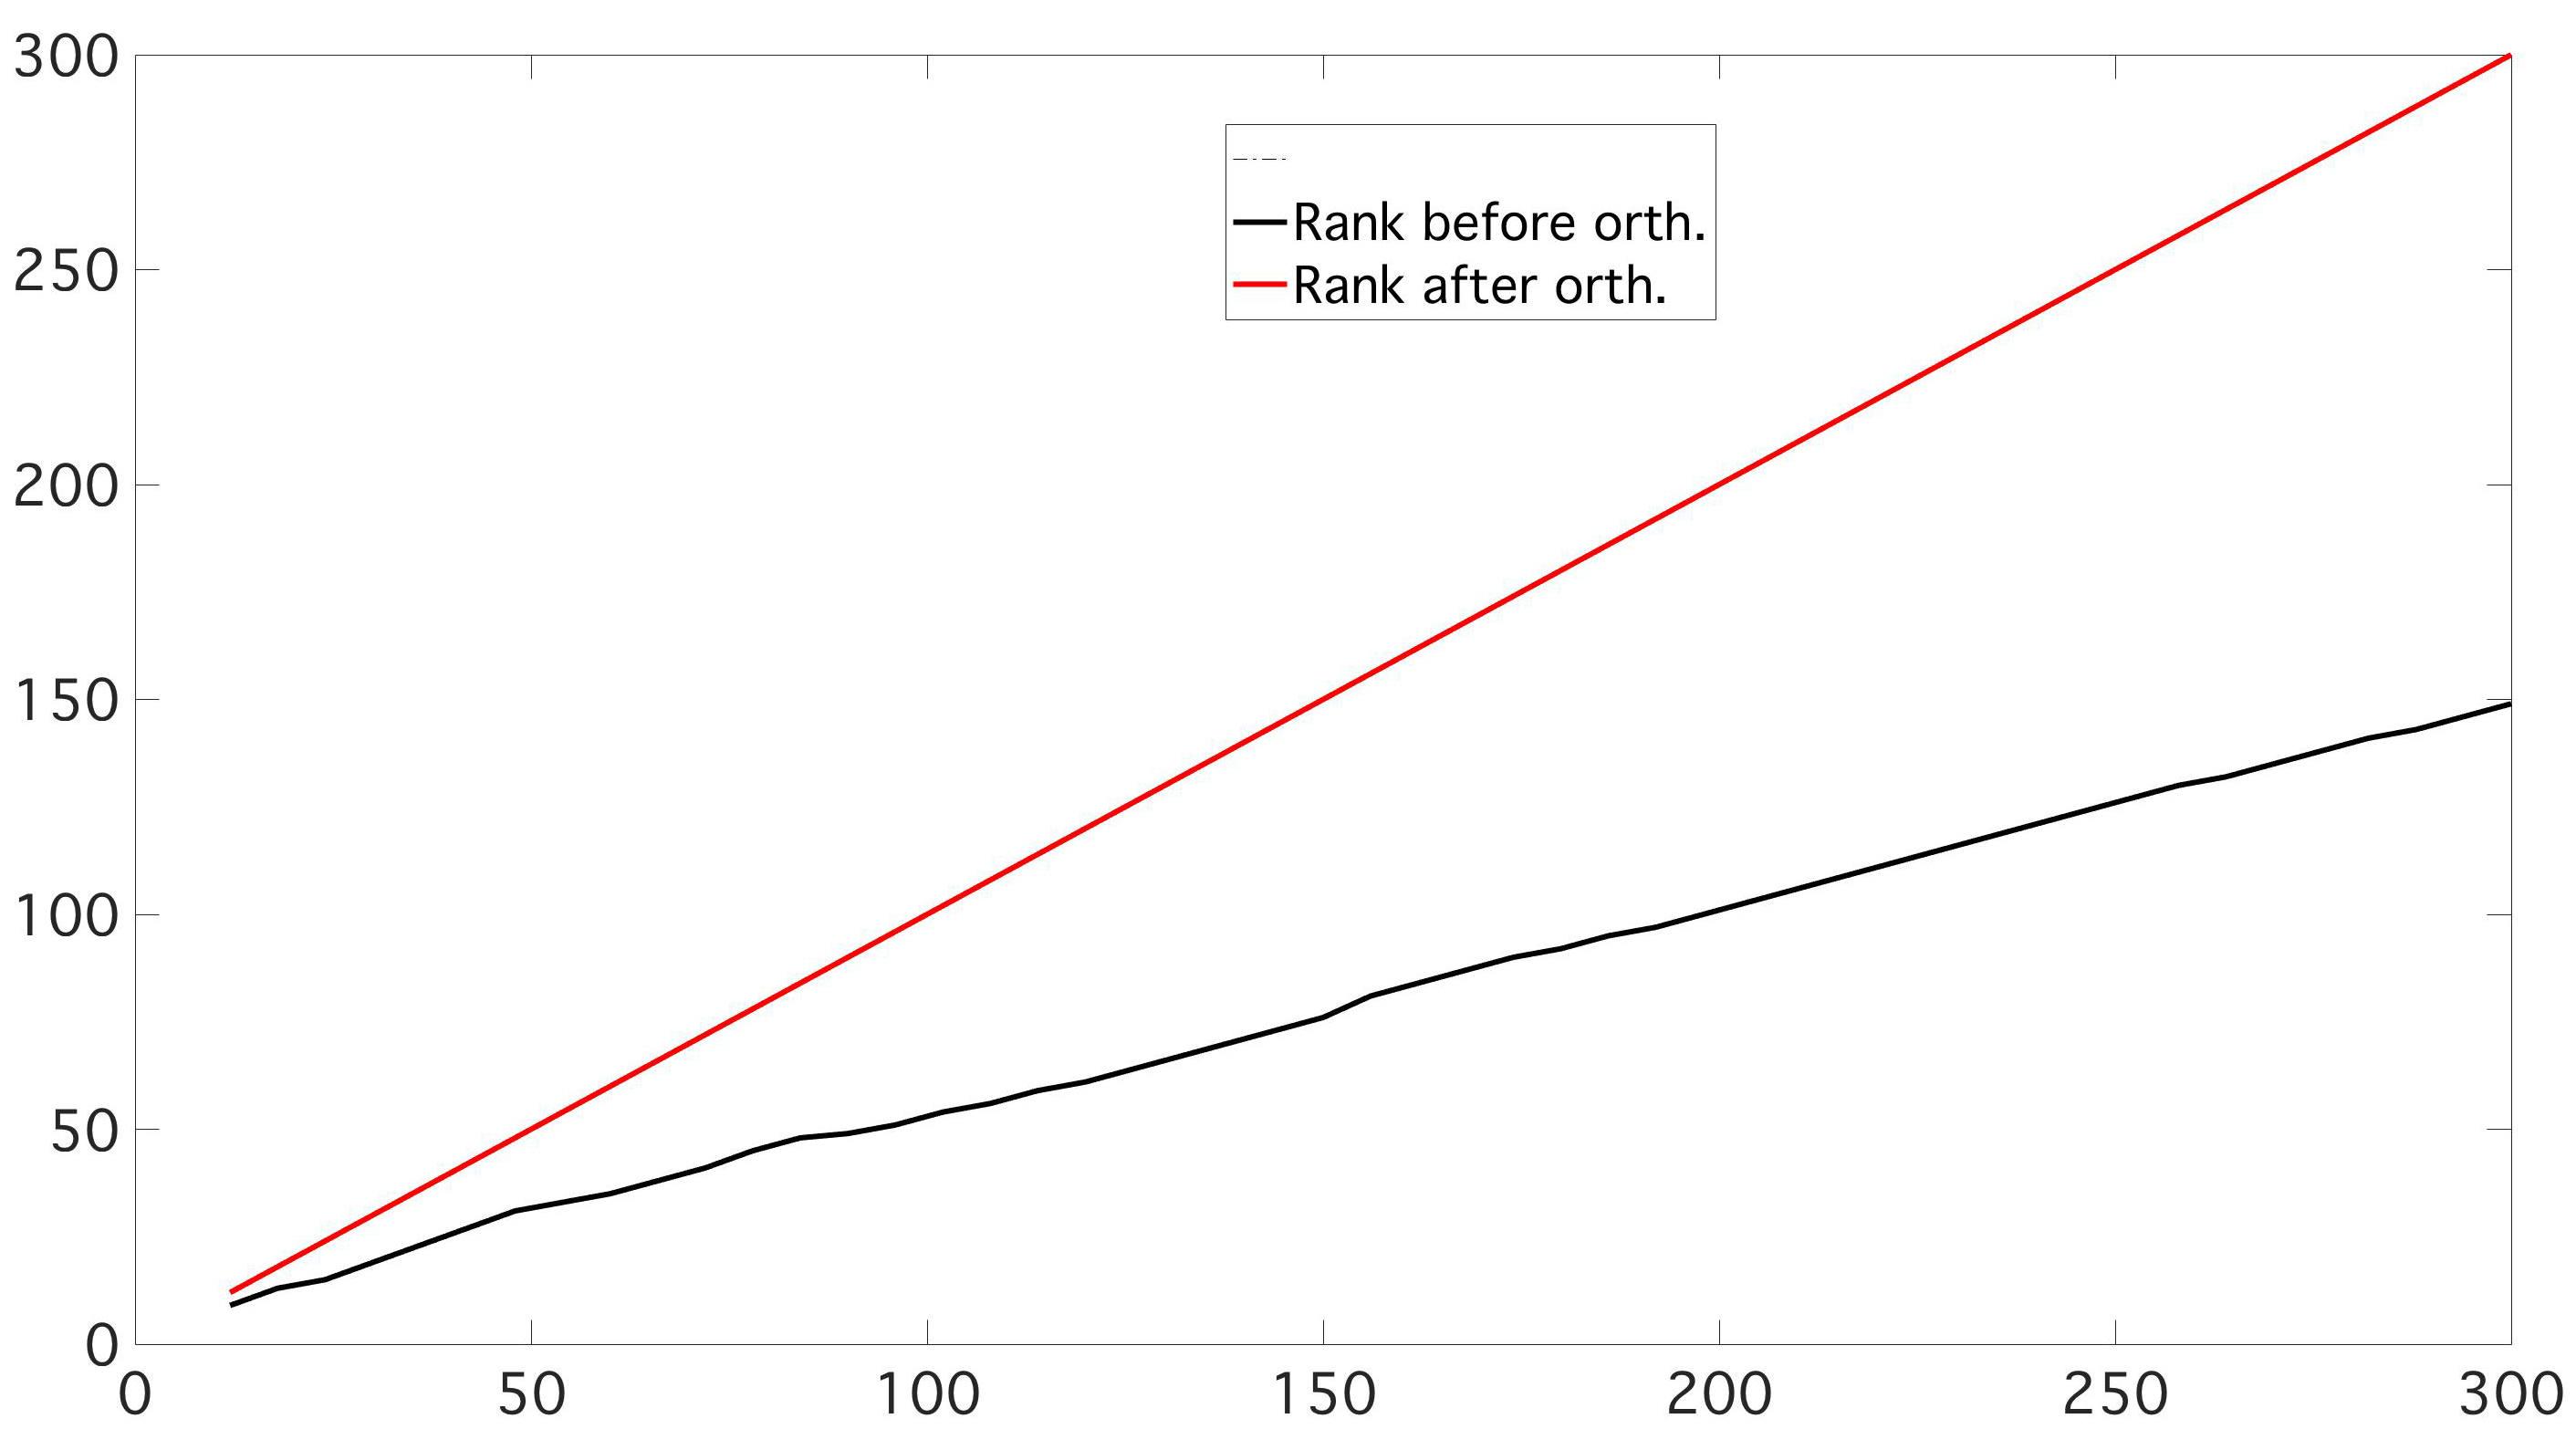
\includegraphics[width=235pt]{FMAP-images/monkey-diffusion-harmonic-laplacian-rank.jpg}
\end{tabular}
\caption{(a,b,$y$-axis) (Black curve) Number of linearly independent functions among (a,b,~$x$-axis) (a) \mbox{$4s$} diffusion functions centred at an increasing number~$s$ (\mbox{$s=1,\ldots,50$}) of uniformly sampled seed points (Fig.~\ref{fig:MONKEY-HARM}a) and at 4 scales (i.e., \mbox{$t=10^{-3},10^{-2},10^{-1},1$}), (b) \mbox{$6s$} functions; i.e.,~$s$ harmonic functions centred at~$s$ seed points,~$s$ Laplacian eigenfunctions, and \mbox{$4s$} diffusion functions at 4 scales (the same as (a)). The diagonal behaviour of the red curves in (a,b) shows that the orthonormalised functions are linearly independent and that the rank-deficiency (black curves) of the input functions is due to (a) small undulations of their values (e.g., at very small scales), (b) the mixture of functions with local (i.e., diffusion functions) and global (i.e., harmonic and Laplacian functions) behaviour.\label{fig:MONKEY-DIFFUSION-RANK}}
\end{figure*}

To show the stability of the diffusion basis functions, let us assume that a perturbation of the input shape corresponds to a perturbation \mbox{$\tilde{\mathbf{L}}_{\epsilon}:=\tilde{\mathbf{L}}+\epsilon\mathbf{E}$} of the Laplacian matrix, with \mbox{$\epsilon\rightarrow 0$}. Indeed, the corresponding diffusion functions become
%
\begin{equation*}
\mathbf{F}(\epsilon)
:=\exp(-t\tilde{\mathbf{L}}_\epsilon)\mathbf{e}_{i},\qquad
\mathbf{F}(0)=\mathbf{K}_{t}\mathbf{e}_{i},
\end{equation*}
%
and the size of the derivative of \mbox{$\mathbf{F}(\epsilon)$} indicates the variation that it undergoes when the Laplacian matrix is perturbed in the direction \mbox{$(\mathbf{E},\epsilon)$}. Assuming that \mbox{$\tilde{\mathbf{L}}\mathbf{E}=\mathbf{E}\tilde{\mathbf{L}}$}\footnote{If \mbox{$\mathbf{A}\mathbf{B}=\mathbf{B}\mathbf{A}$}, then \mbox{$\exp(\mathbf{A}+\mathbf{B})=\exp(\mathbf{A})\exp(\mathbf{B})$} and \mbox{$\mathbf{A}\exp(\mathbf{B})=\mathbf{B}\exp(\mathbf{A})$}.} and differentiating the previous equation, we get that
%
\begin{equation*}
\mathbf{F}^{\prime}(\epsilon)
:=t\exp(-t\tilde{\mathbf{L}}_\epsilon)\mathbf{E}\mathbf{e}_{i},\qquad
\mathbf{F}^{\prime}(0)
:=t\exp(-t\tilde{\mathbf{L}})\mathbf{E}\mathbf{e}_{i}.
\end{equation*}
%
Then, we obtain the upper bound
%
\begin{equation*}
\begin{split}
\|\mathbf{F}^{\prime}(0)\|_{2}
%&\leq t\|\exp(-t\tilde{\mathbf{L}})\mathbf{E}\mathbf{e}_{i}\|_{2}\\
\leq t\|\exp(-t\tilde{\mathbf{L}})\|_{2}\,\|\mathbf{E}\|_{2}\,\|\mathbf{e}_{i}\|_{2}
%&\leq t\,\|\mathbf{E}\|_{2}\,\|\mathbf{e}_{i}\|_{2}\\
\leq t\,\|\mathbf{E}\|_{2},
\end{split}
\end{equation*}
%
which implies that the computation of the diffusion basis functions is stable with respect to perturbations of the input surface.

\subsection{Selection of the seed points\label{sec:SEED-SELECTION}}
The definition of the harmonic and diffusion basis functions involve the selection of a set of seed points, which allow us to adapt the behaviour of the corresponding basis functions to the local geometry of the input shape, by choosing a set of feature points (e.g,, high-curvature points, surface samples) or a set of landmarks for the computation of the functional map. In fact, the maximum principle for the harmonic and diffusion equations guarantee that the corresponding solution will have a maximum at the selected seed points.

Since the diffusion basis functions are compactly-supported at small scales, the coverage of the whole surface with their supports depends on the selected seeds and on the support of each basis function. Increasing the number of seed points, or the scale~$t$, all the vertices of the input surface will belong to the support of one or more basis functions.

To guarantee the coverage of the whole surface with the supports of the diffusion functions at a given scale, we proceed in the following way. At the first step, we select a seed point (e.g., a point of maximum curvature) and define~$k$ (e.g., \mbox{$k:=10$}, in our experiments) seed points by applying the farthest point sampling method~\citep{ELDAR2007,MOENNING2003}. Then, the number of seed points is iteratively increased until the supports of the basis functions cover the whole surface. Since we use a set of multiple scales, the union of the supports of all the diffusion functions always cover the whole surface.

\subsection{Scale-invariance of the basis functions\label{sec:ISOMETRY-INVARIANCE}}
We now discuss the scale-invariance of the harmonic and diffusion basis functions.

\paragraph*{Harmonic basis functions}
The discrete harmonic basis functions are scale-invariant; in fact, the stiffness matrix with cotangent weights is not affected by a uniform re-scaling of the input surface.

\paragraph*{Diffusion basis functions}
Reshaping the input surface~$\mathcal{M}$ to \mbox{$\alpha\mathcal{M}$}, the mass matrix~$\mathbf{B}$ and the eigen-system \mbox{$(\lambda_{i},\mathbf{x}_{i})_{i=1}^{n}$} of~$\mathcal{M}$ become \mbox{$\alpha^{2}\mathbf{B}$} and \mbox{$(\alpha^{-2}\lambda_{i},\alpha^{-1}\mathbf{x}_{i})_{i=1}^{n}$}, respectively. Recalling the spectral representation (\ref{eq:EIGS-SPECTRAL-OP}) of the diffusion basis function, we get the identity \mbox{$\mathbf{K}_{t}^{\alpha\mathbf{M}}\mathbf{e}_{i}=\mathbf{K}_{\alpha^{-2}t}^{\mathbf{M}}\mathbf{e}_{i}$}. Indicating with \mbox{$\vert\mathcal{M}\vert$} the area of~$\mathcal{M}$ and rescaling the time parameter to \mbox{$\vert\mathcal{M}\vert t$}, we get that \mbox{$\mathbf{K}_{\vert\mathcal{M}\vert t}^{\alpha\mathcal{M}}\mathbf{e}_{i}=\mathbf{K}_{t}^{\mathcal{M}}\mathbf{e}_{i}$}; i.e., \mbox{$\mathbf{K}_{\vert\mathcal{M}\vert t}\mathbf{e}_{i}$} is the \emph{scale-invariant diffusion function} centred at~$\mathbf{p}_{i}$.

\subsection{Orthonornalisation of the basis functions\label{sec:ORTHONOTMALIZATION-PROCESS}}
Selecting~$k$ points, \mbox{$2\leq k\leq n$}, then we generate~$k$ harmonic basis functions and~$k$ diffusion basis functions at a given scale~$t$. Choosing~$s$ scales, which should be small and large in order to encode local and global shape/signal properties, we obtain \mbox{$sk$} diffusion basis functions. Selecting multiple scales or stacking different types of basis functions, we define a richer functional space for the computation of the functional map, by encoding different geometric properties of the input domain. In these cases, we must check that they are still linearly independent and select a subset of linear independent and/or orthonormal. To this end, we apply the Gram-Schmidt method (Sect.~\ref{sec:GM-ORHTONORMALIZAION}) or the QR factorisation (Sect.~\ref{sec:QR-ORHTONORMALIZAION}).

\paragraph*{Stack of basis functions}
If we stack different types of basis functions in a matrix~$\mathbf{Y}$, then we insert the diffusion functions from small to large scales as first elements of the stack. Successively, we include harmonic and Laplacian functions. In case of linearly dependent functions in the stack, the QR orthonormalisation will preserve all the diffusion basis functions in~$\mathbf{Y}$, as they are linearly independent. Then, it will generate a subset of new orthonormal functions from the remaining (harmonic, Laplacian) functions. From the point of view of the preservation of the locality of the support of the input functions, the position of the harmonic and Laplacian functions is interchangeable in the stack. For the functional map framework, we generally prefer to have basis functions centred at seed points; indeed, we place the harmonic functions after the diffusion ones. 
%
\begin{figure*}
\centering
\begin{tabular}{ll}
Mean correspondence error & Mean Correspondence error\\
(a)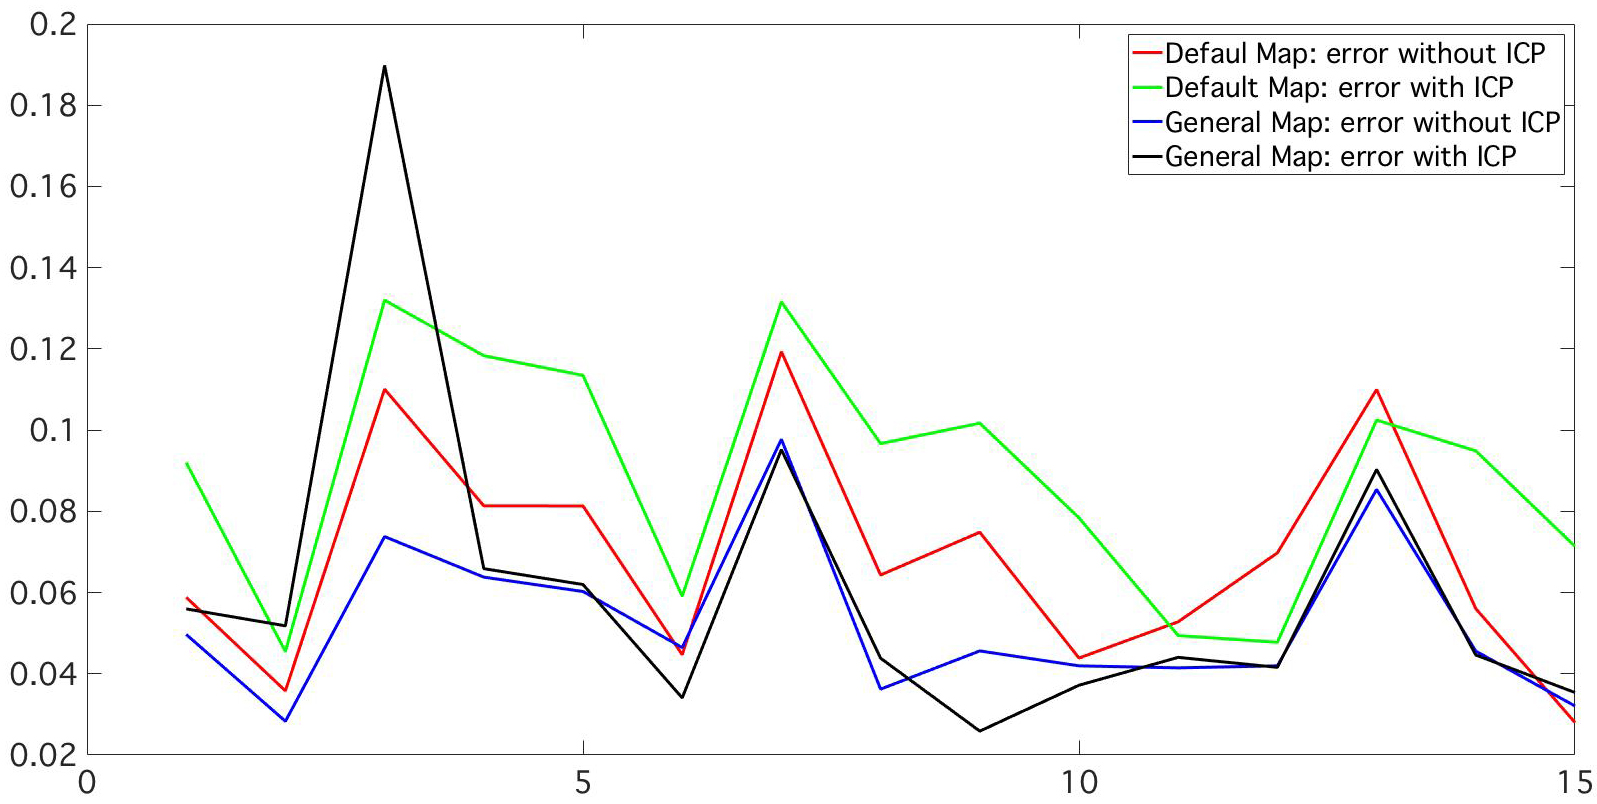
\includegraphics[height=120pt]{FMAP-images/19-STATISTICS-A.jpg}
&(b)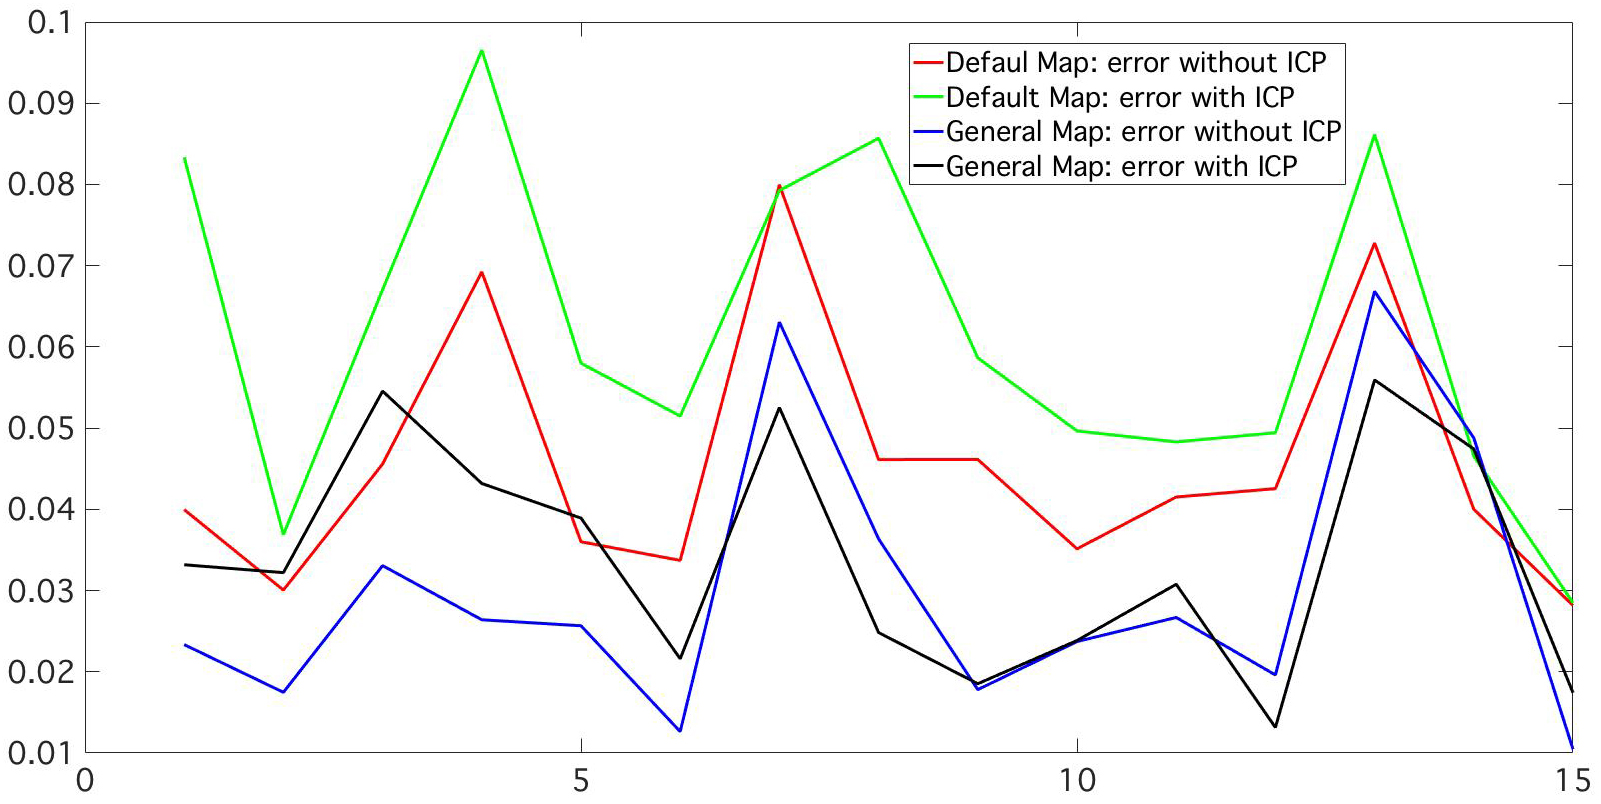
\includegraphics[height=120pt]{FMAP-images/19-STATISTICS-B.jpg}\\
48 Diffusion funct. (7 ground-truth landm., 5 seeds)
&60 Diffusion funct. (10 ground-truth landm., 5 seeds)\\
60 Laplacian eigenfunc.
&60 Laplacian eigenfunc.
\end{tabular}
\begin{tabular}{ccc}
\hline
\multicolumn{3}{c}{Diffusion basis}\\
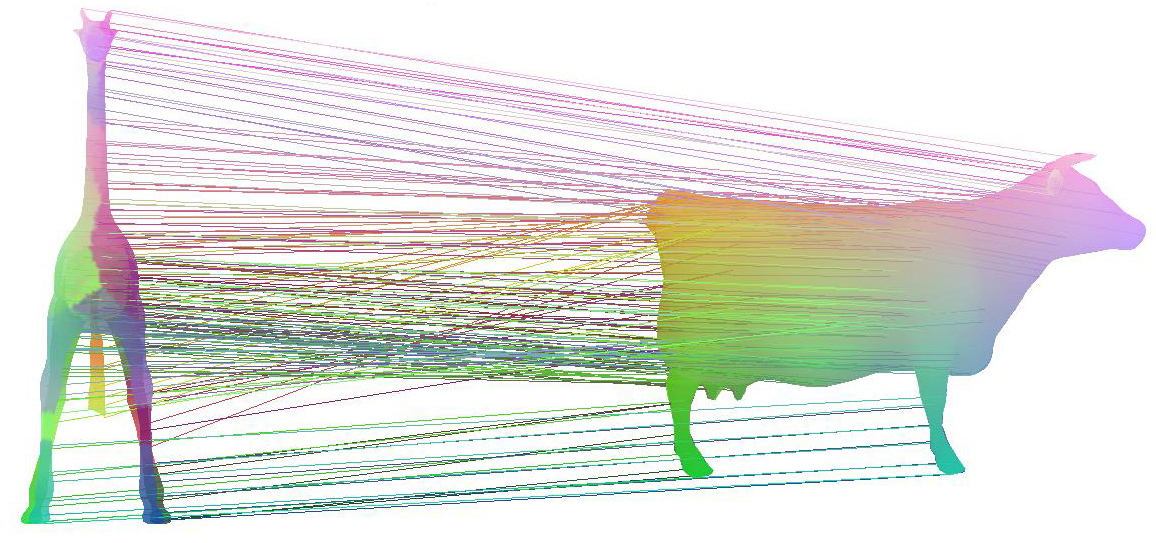
\includegraphics[height=65pt]{FMAP-images/4legs-Source=381-Target=390-General-Basis-ZOOM.jpg}
&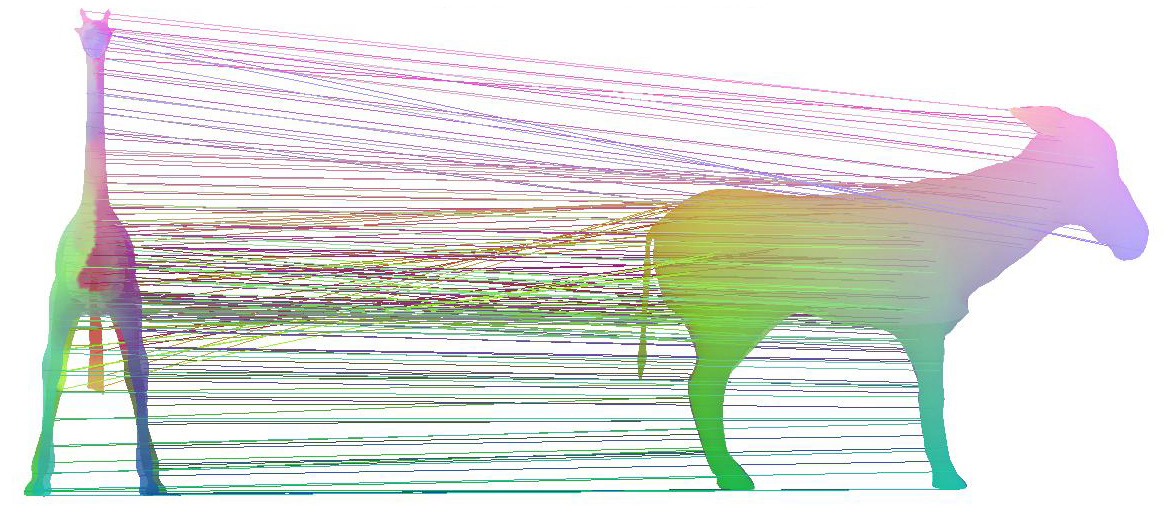
\includegraphics[height=65pt]{FMAP-images/4legs-Source=385-Target=390-General-Basis-ZOOM.jpg}
&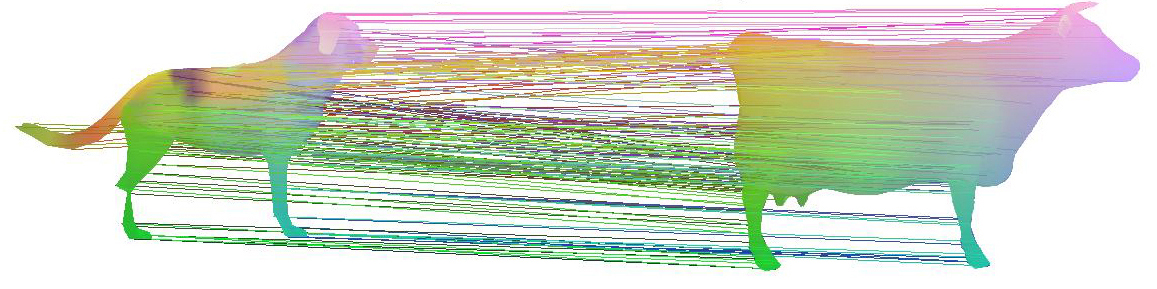
\includegraphics[height=50pt]{FMAP-images/4legs-Source=381-Target=398-General-Basis-ZOOM.jpg}\\
\hline
\multicolumn{3}{c}{Laplacian eigenbasis}\\
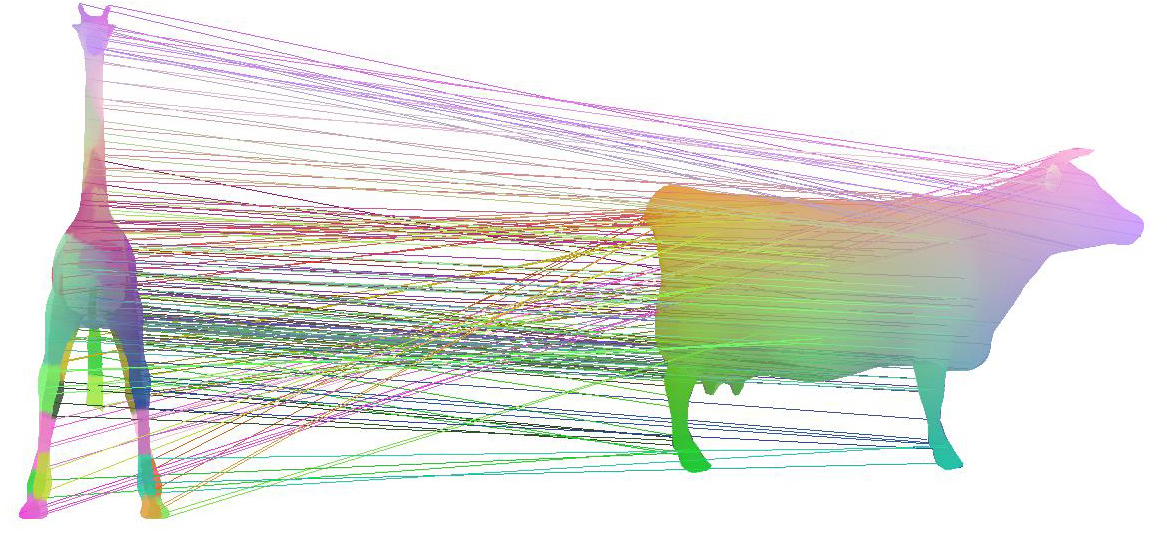
\includegraphics[height=65pt]{FMAP-images/4legs-Source=381-Target=390-Lapl-Eig-ZOOM.jpg}
&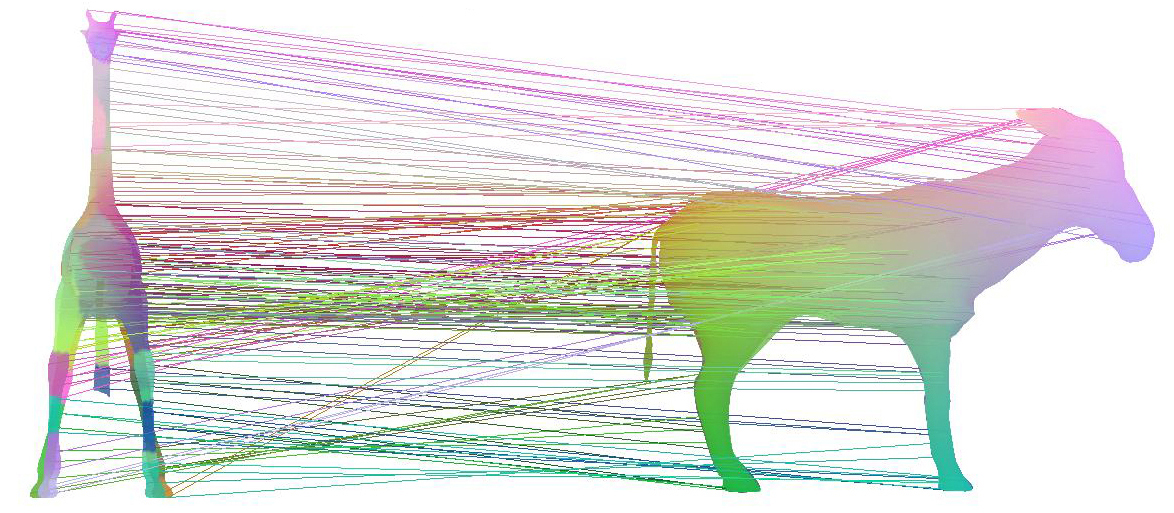
\includegraphics[height=65pt]{FMAP-images/4legs-Source=385-Target=390-Lapl-Eig-ZOOM.jpg}
&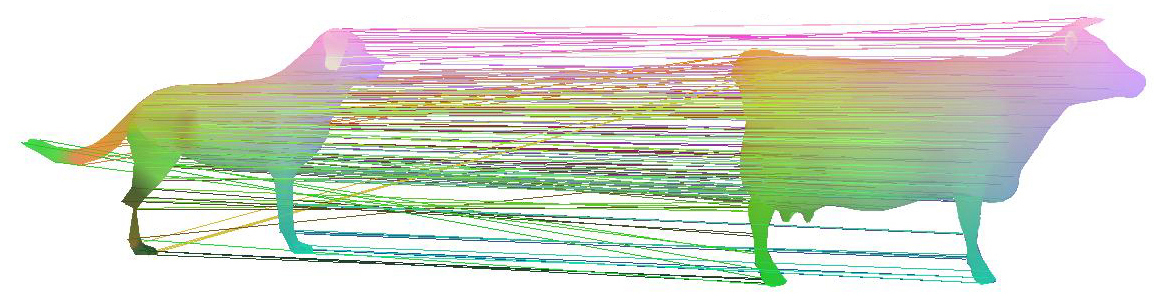
\includegraphics[height=50pt]{FMAP-images/4legs-Source=381-Target=398-Lapl-Eig-ZOOM.jpg}
%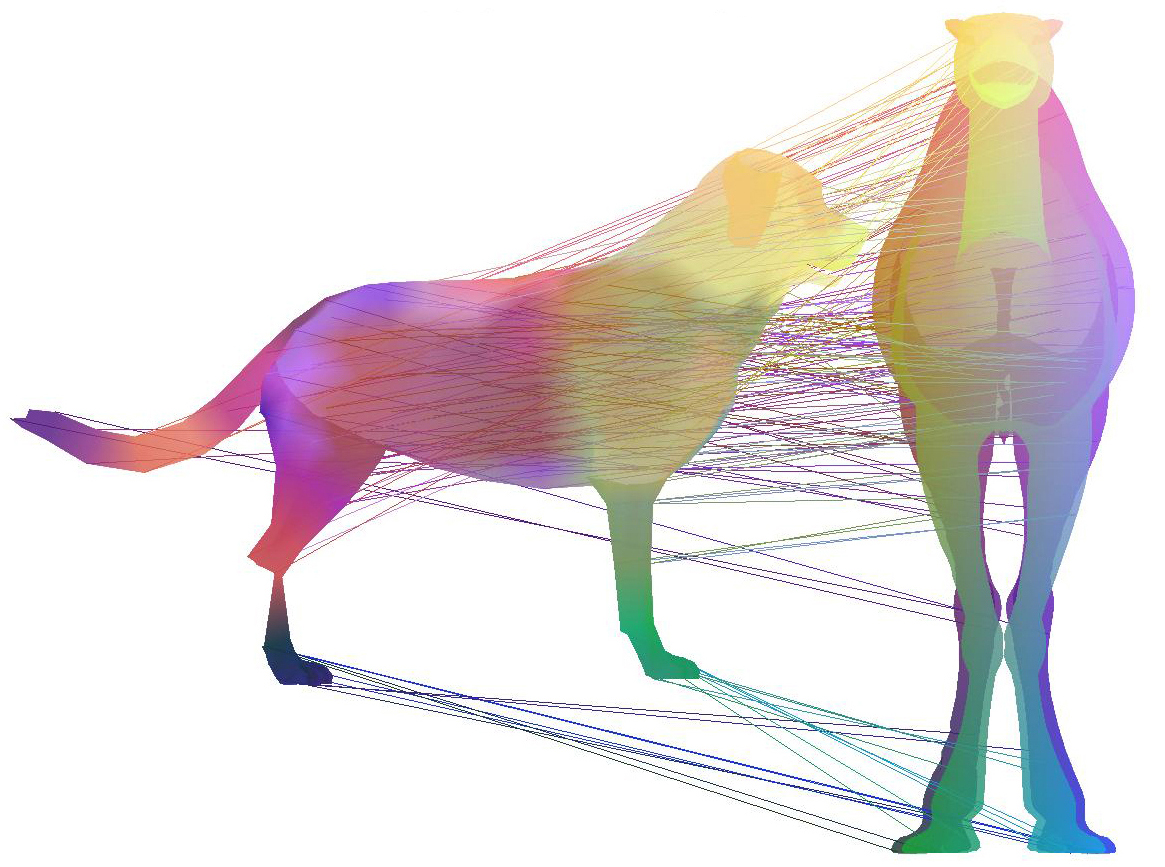
\includegraphics[height=100pt]{FMAP-images/4legs-Source=393-Target=398-General-Basis-ZOOM.jpg}
%&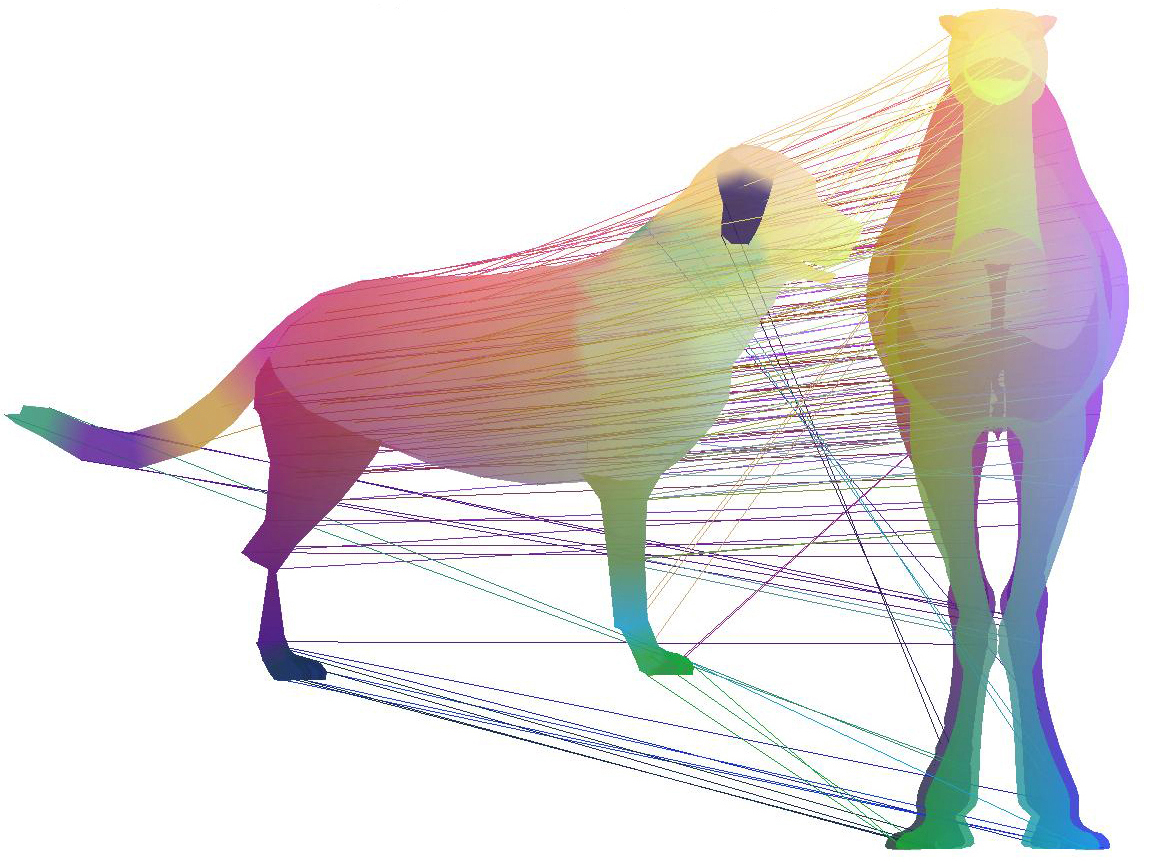
\includegraphics[height=100pt]{FMAP-images/4legs-Source=393-Target=398-Lapl-Eig-ZOOM.jpg}
\end{tabular}
\caption{(a,b,~$y$-axis) Mean correspondence error on 15 couples ($x$-axis) of shapes belonging to the 4-legs class of the SHREC data set computed with (a) 48, (b) 60 diffusion functions (4 scales, (a,b) 5 seed points, (a) 7 and (b) 10 ground-truth landmarks) and (a,b) 60 Laplacian eigenfunctions. The diffusion functions generally provide a lower correspondence error before/after ICP, and improves the quality of the correspondences with respect to the Laplacian eigenbasis; e.g., on (left) the legs of the giraffe and the tail of the cow, (middle) the legs of the giraffe and the horns of the goat, (right) the legs of the dog and the horns of the cow. A small increase of the number (from 7 to 10) of landmarks reduces the mean correspondence error approximately of the \mbox{$50\%$}. With reference to (a), the improvement of the shape correspondences (2nd, 3rd rows) is also due to the multi-scale nature of the diffusion functions.\label{fig:4LEGS-DIFFUSION-CORRESPONDENCES}}
\end{figure*}
%
\subsubsection{Gram-Schimdt orthonormalisation\label{sec:GM-ORHTONORMALIZAION}}
We assume that we already have a set \mbox{$\mathcal{B}:=(\mathbf{u}_{i})_{i=1}^{n}$} of linearly independent (discrete) functions; for instance, a set of diffusion basis functions at a scale~$t$, or a set of harmonic basis functions at seed points. All these functions are linearly independent by construction but not necessarily orthonormal. The Gram-Schmidt orthonormalisation process is applied to compute an orthonormal set of functions \mbox{$\tilde{\mathcal{B}}:=(\mathbf{w}_{i})_{i=1}^{n}$}, which generate the same space of scalar function as~$\mathcal{B}$. In the standard approach, the set~$\tilde{\mathcal{B}}$ is computed from~$\mathcal{B}$ through an iterative procedure that is generally subject to numerical instabilities and that leads to inaccurate and non-orthonormal functions.

We briefly recall the main steps of a variant of this orthonormalisation, which processes the input functions simultaneously instead of sequentially and will be useful to understand how it might influence the supports of the input functions. At the first iteration, we initialise the function \mbox{$\mathbf{u}_{1}:=\mathbf{w}_{1}/\|\mathbf{w}_{1}\|_{\mathbf{B}}$}, and we then recursively compute the functions
%
\begin{equation}\label{eq:ORTH-VECTORS}
\left\{
\begin{array}{l}
\mathbf{w}_{k}^{(j+1)}:=\mathbf{w}_{k}^{(j)}-\langle\mathbf{w}_{k}^{(j)},\mathbf{u}_{j}\rangle_{\mathbf{B}}\mathbf{u}_{j},\qquad
\mathbf{u}_{j}
:=\frac{\mathbf{w}_{j}^{(j)}}{\|\mathbf{w}_{j}^{(j)}\|_{\mathbf{B}}};\\
j=1,\ldots,n-1,\quad k=j+1,\ldots,n.
\end{array}
\right.
\end{equation}
%
At the last iteration, we compute \mbox{$\mathbf{u}_{n}:=\mathbf{w}_{n}^{(n)}/\|\mathbf{w}_{n}^{(n)}\|_{\mathbf{B}}$}. 

By definition, a set of functions with no overlapping supports are always orthogonal with respect to the~$\mathbf{B}$-scalar product. At large scales, or in case of harmonic/Laplacian functions, the intersection among the supports of the input functions will imply that they are no more orthonormal and will be linearly combined according to Eq. (\ref{eq:ORTH-VECTORS}) in order to make them orthonormal. If the supports of the functions have empty or small intersections with respect to the surface area, then the iterations (\ref{eq:ORTH-VECTORS}) will not alter the support of the input functions, thus preserving their locality. In fact, the support of~$\mathbf{w}_{k}^{(j+1)}$ will depend on the intersection (if any) between the support of~$\mathbf{w}_{k}^{(j)}$ and~$\mathbf{u}_{j}$.
%
\begin{figure*}
\begin{tabular}{c|c|c}
Mean correspondence error &Diffusion basis &Laplacian eigenbasis\\
\hline
(a)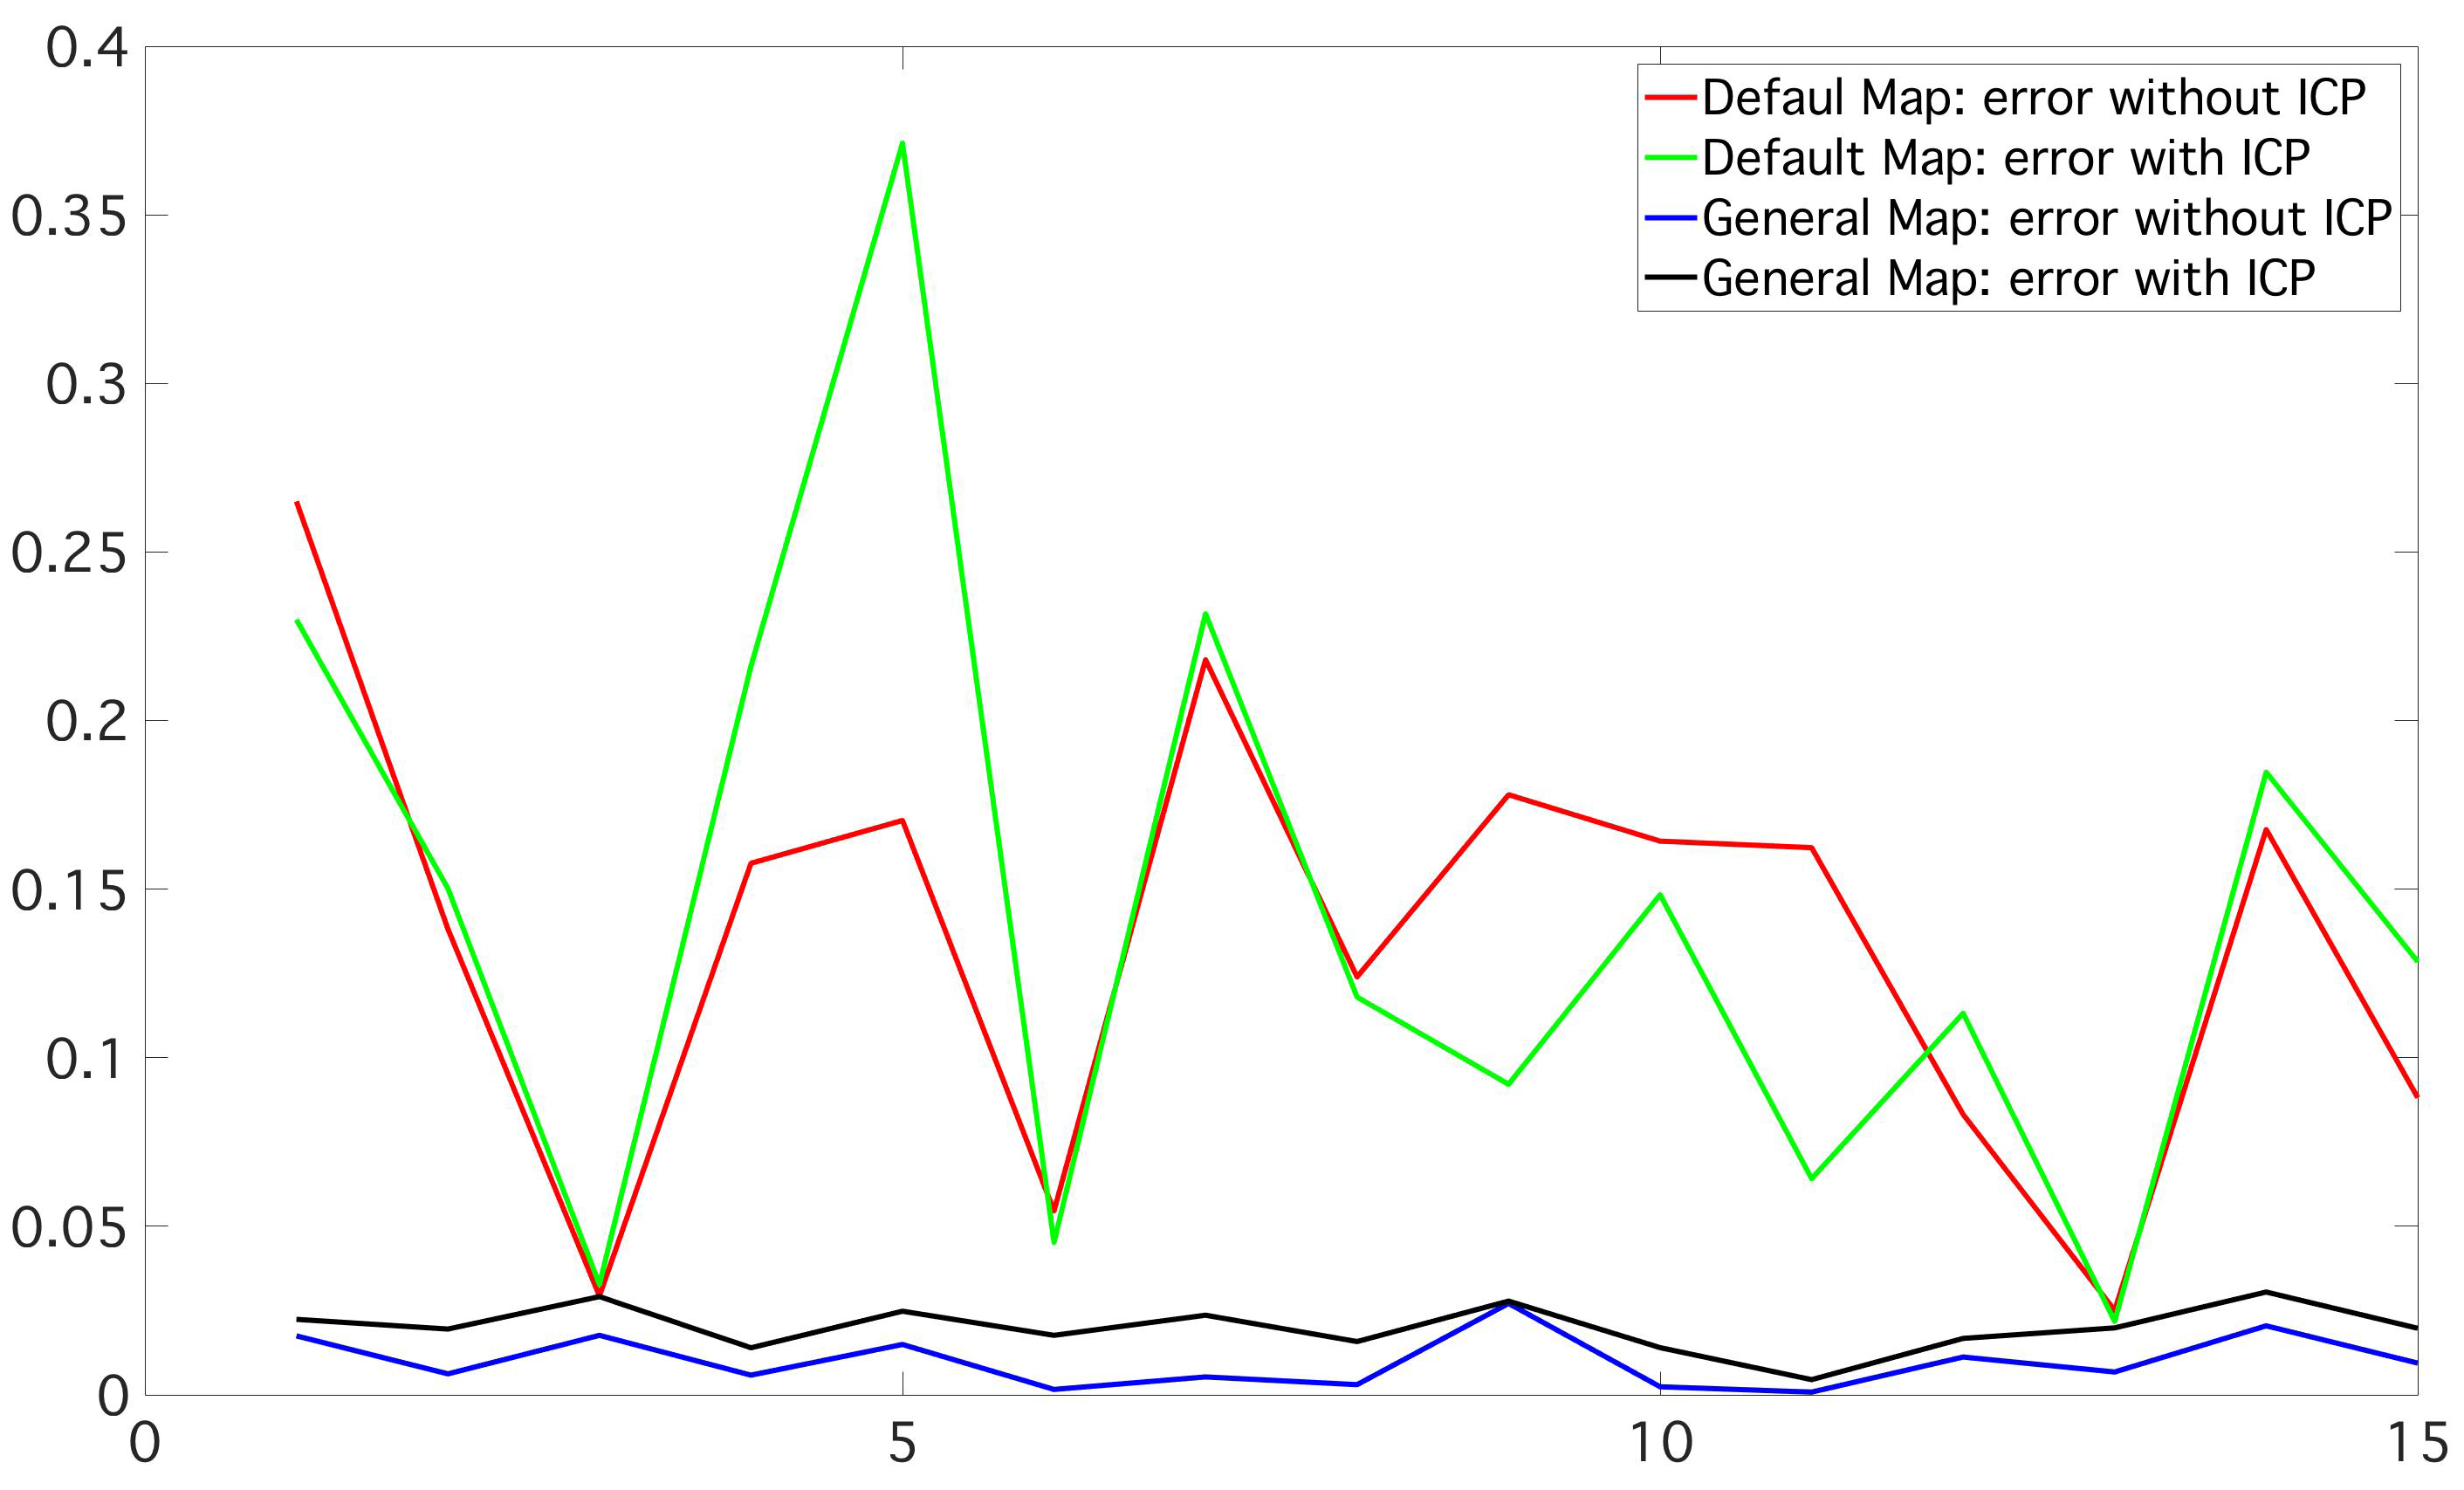
\includegraphics[height=105pt]{FMAP-images/plane-STATISTICS.jpg}
&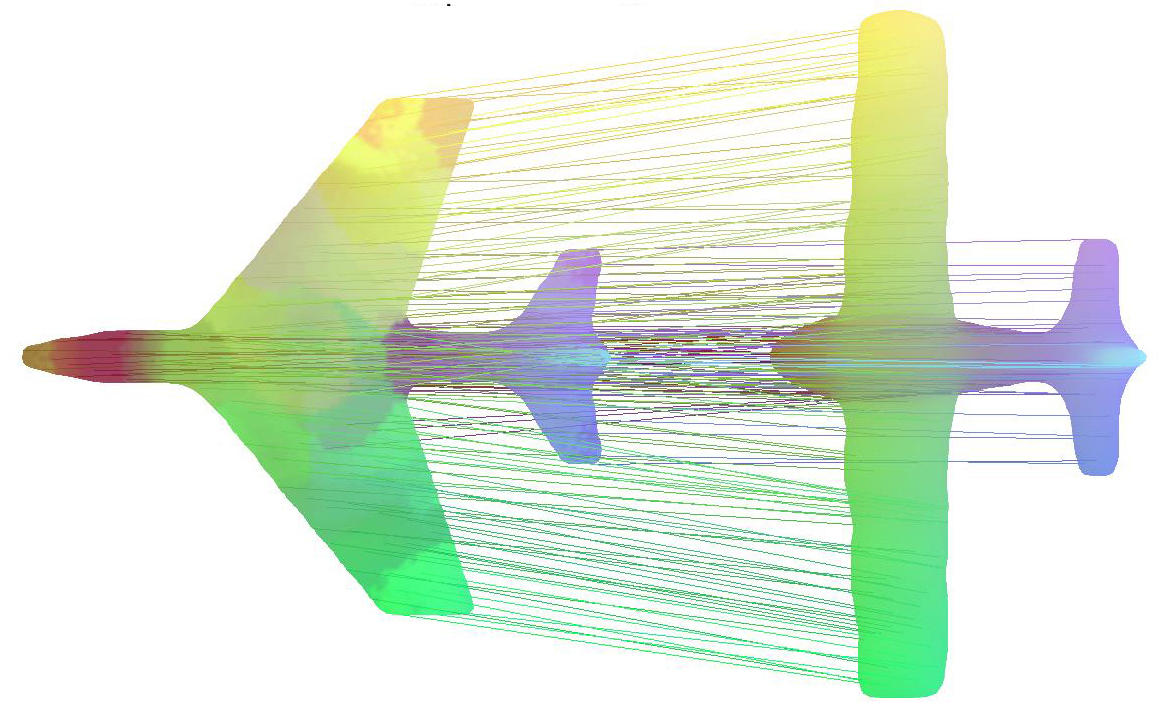
\includegraphics[height=85pt]{FMAP-images/plane-Source=61-Target=66-General-Basis.jpg}
&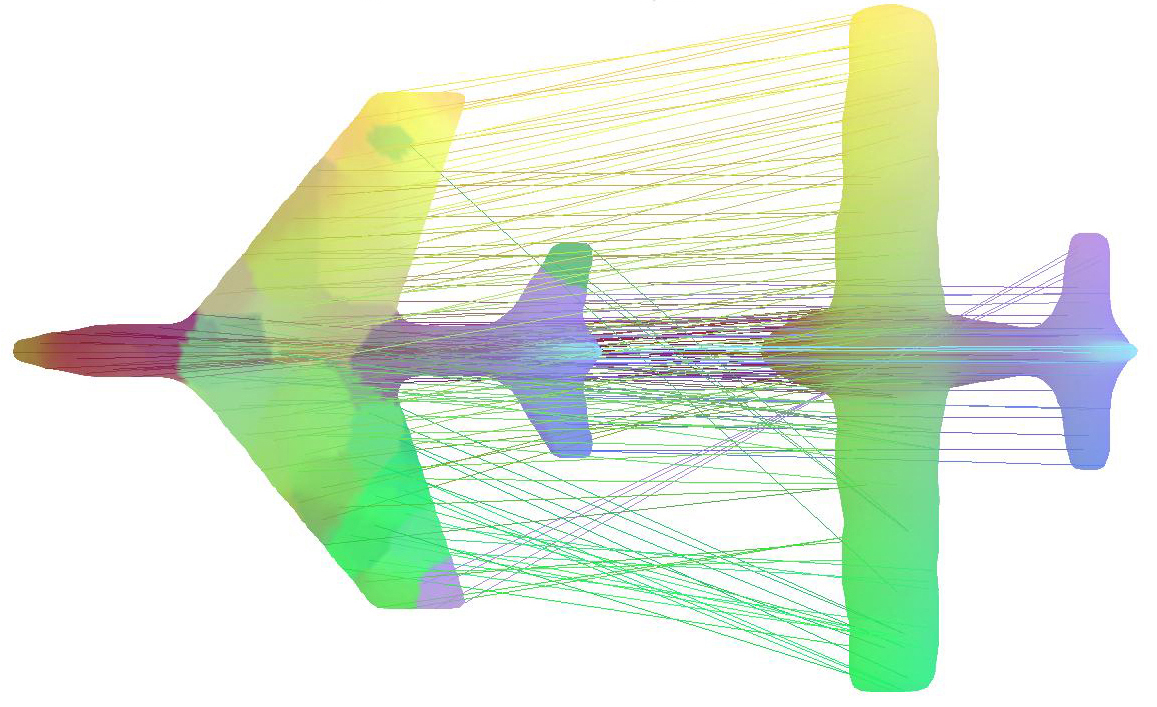
\includegraphics[height=85pt]{FMAP-images/plane-Source=61-Target=66-Lapl-Eig-ZOOM.jpg}\\
(b)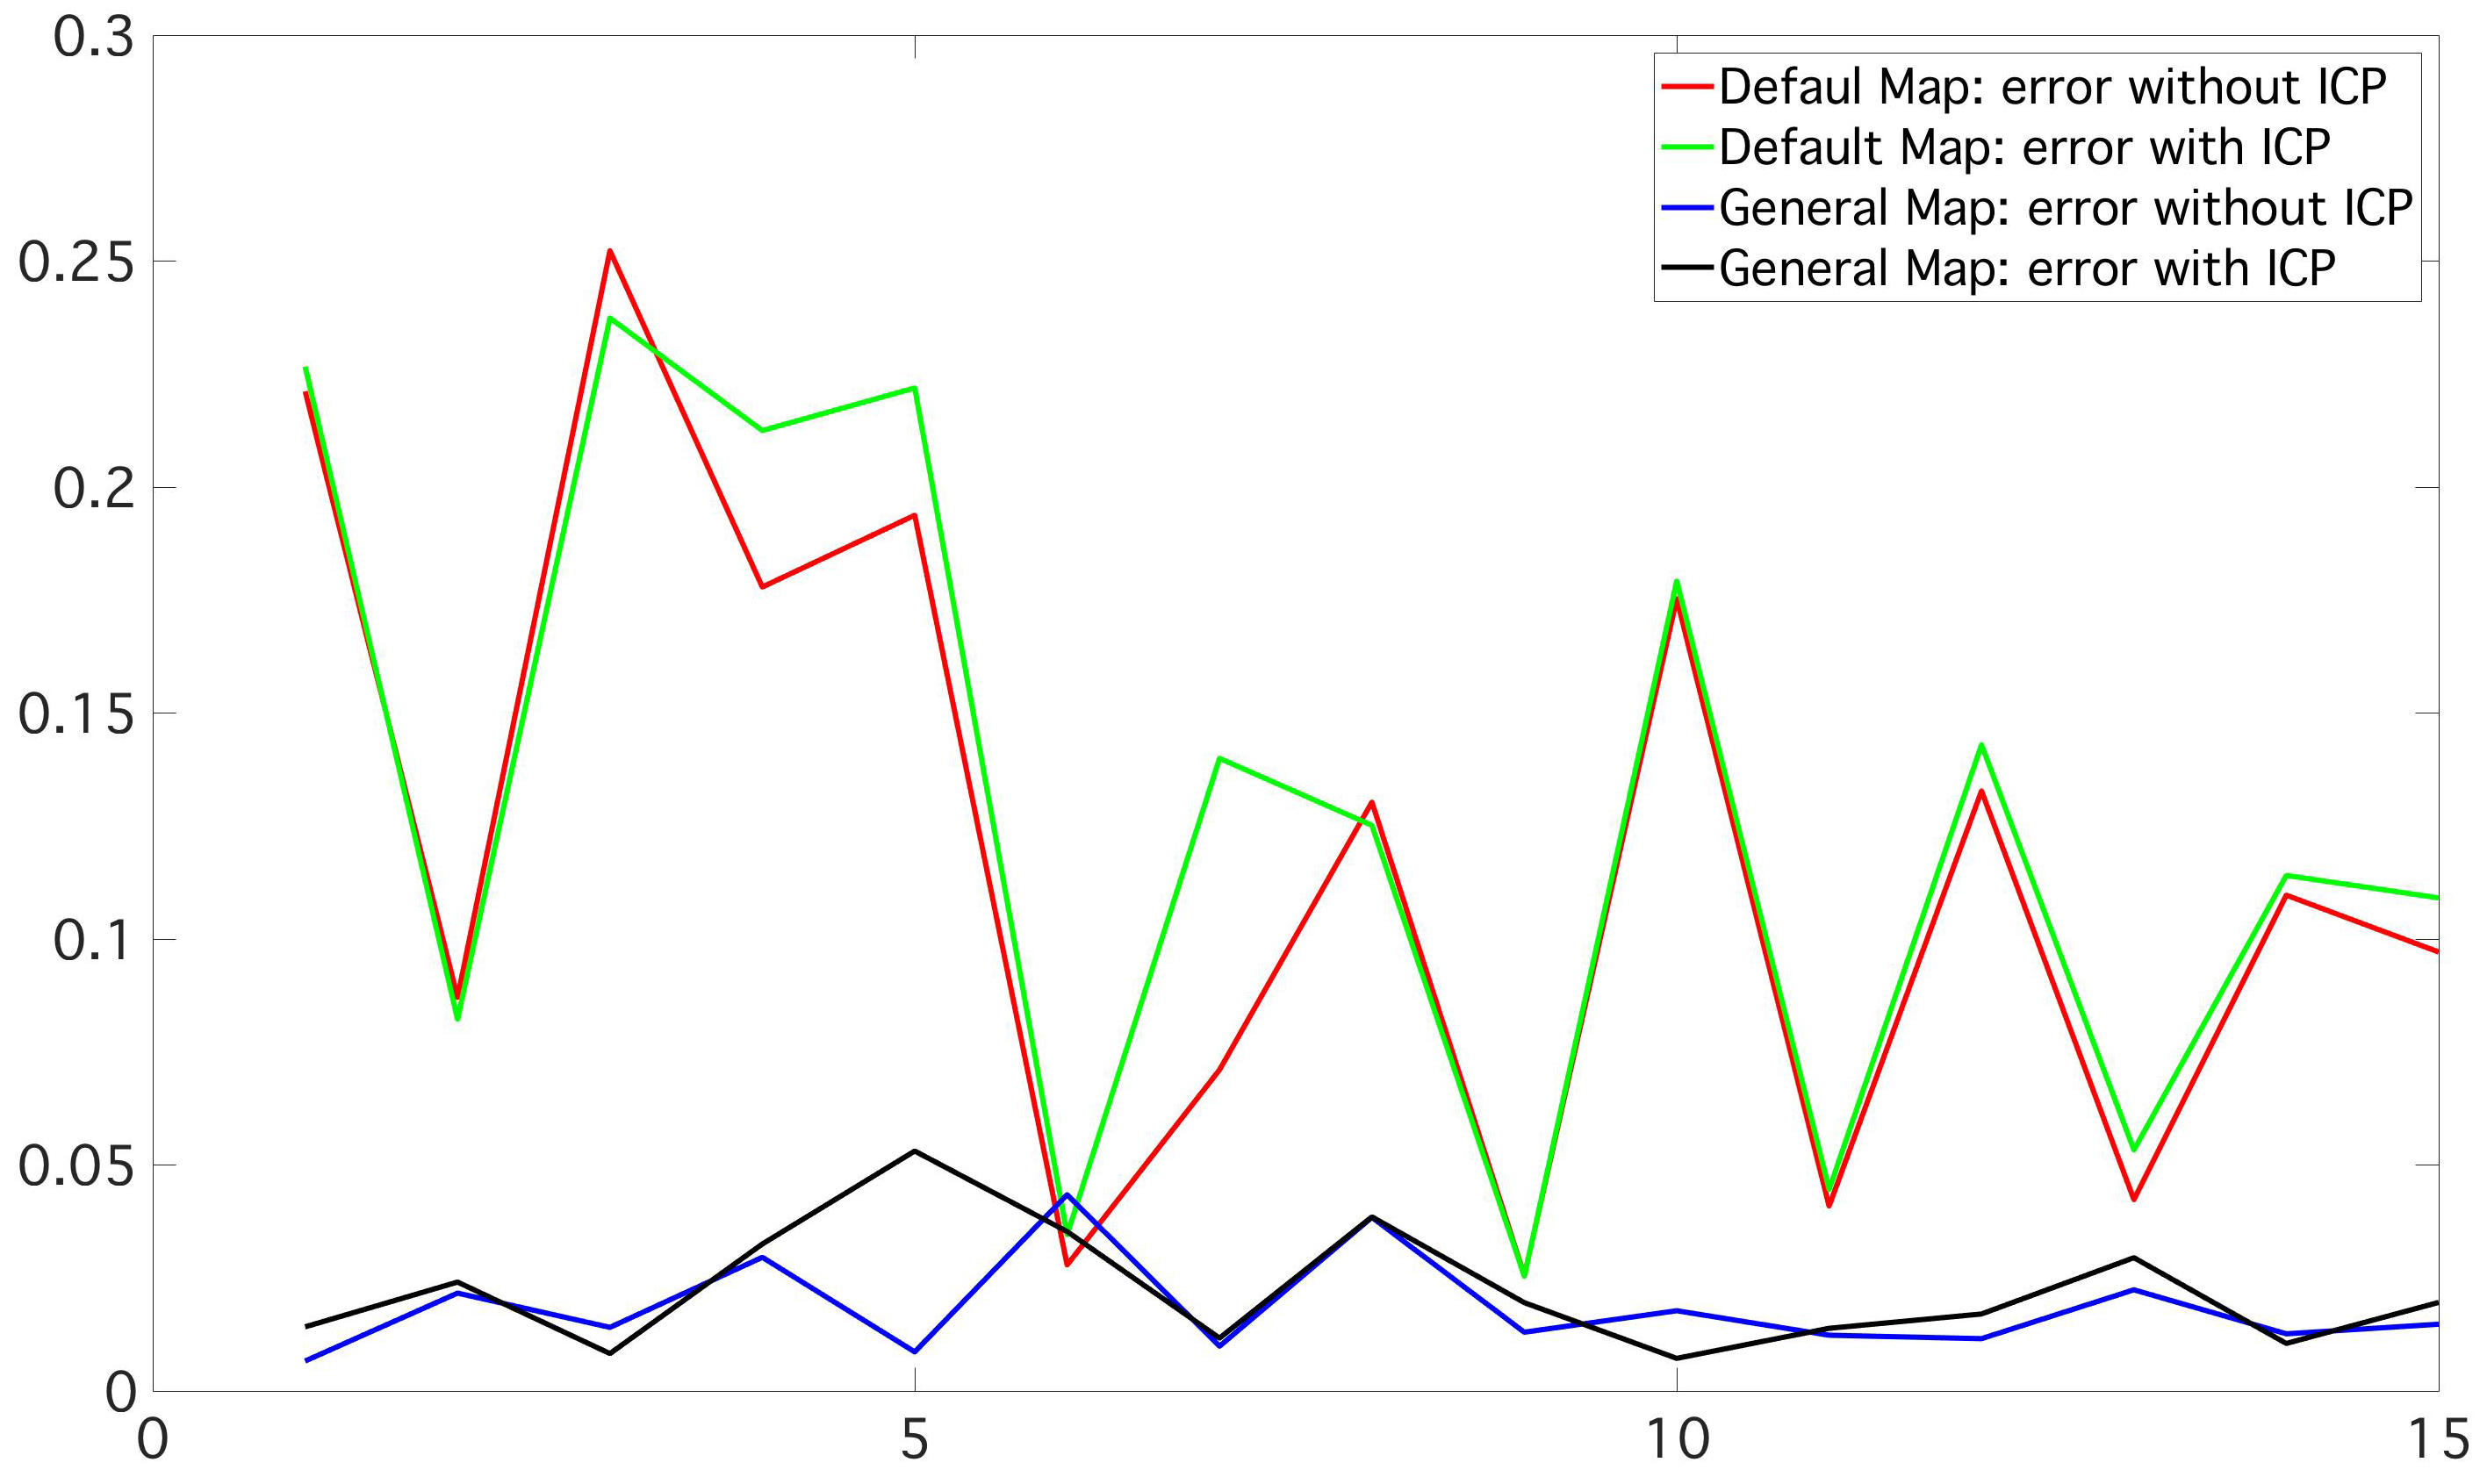
\includegraphics[height=105pt]{FMAP-images/table-STATISTICS.jpg}
&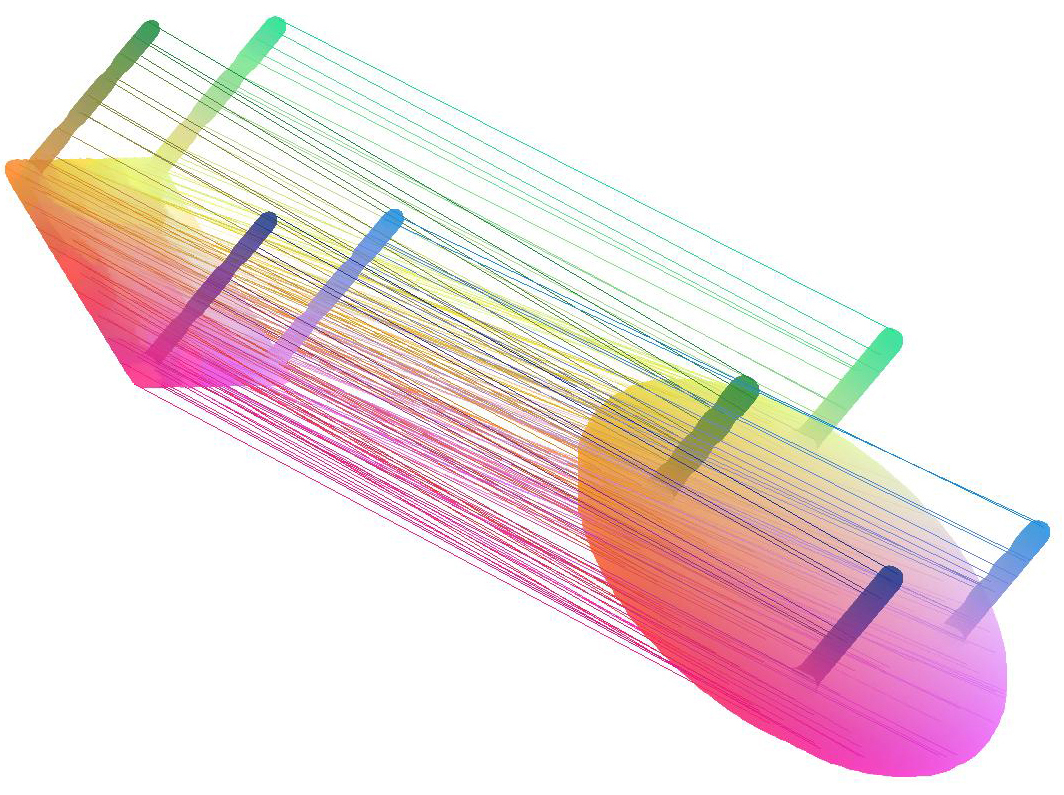
\includegraphics[height=85pt]{FMAP-images/table-Source=157-Target=158-General-Basis-ZOOM.jpg}
&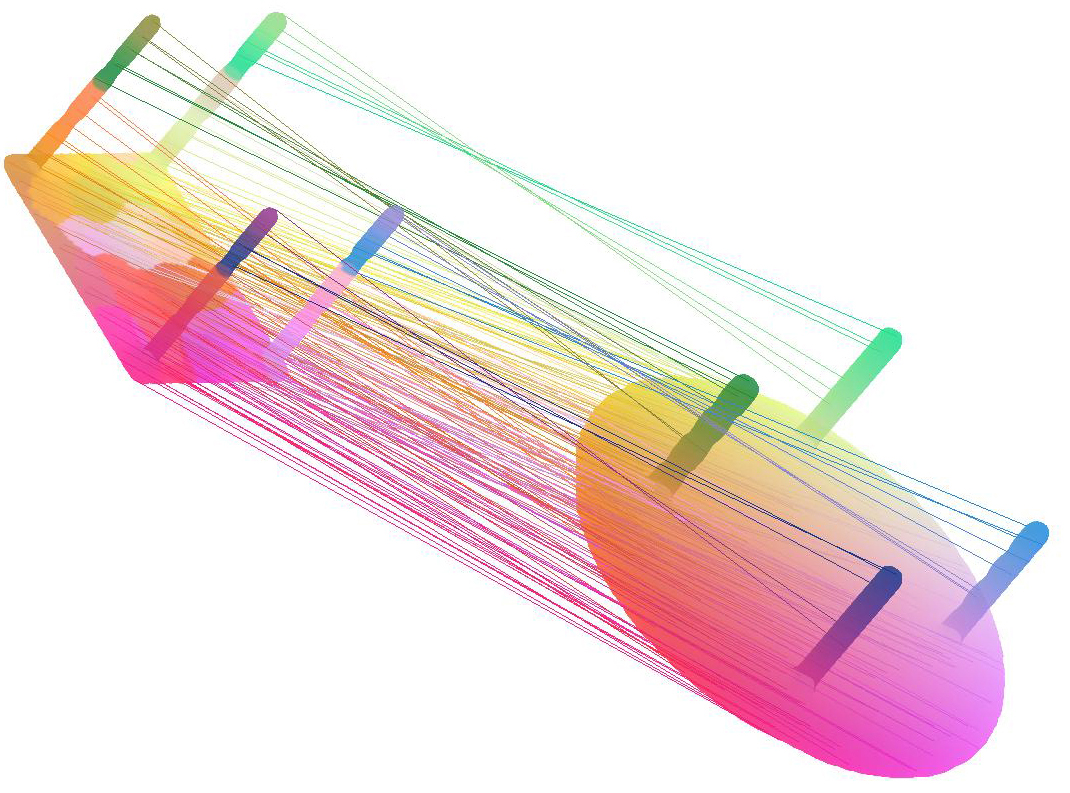
\includegraphics[height=85pt]{FMAP-images/table-Source=157-Target=158-Lapl-Eig-ZOOM.jpg}\\
(c)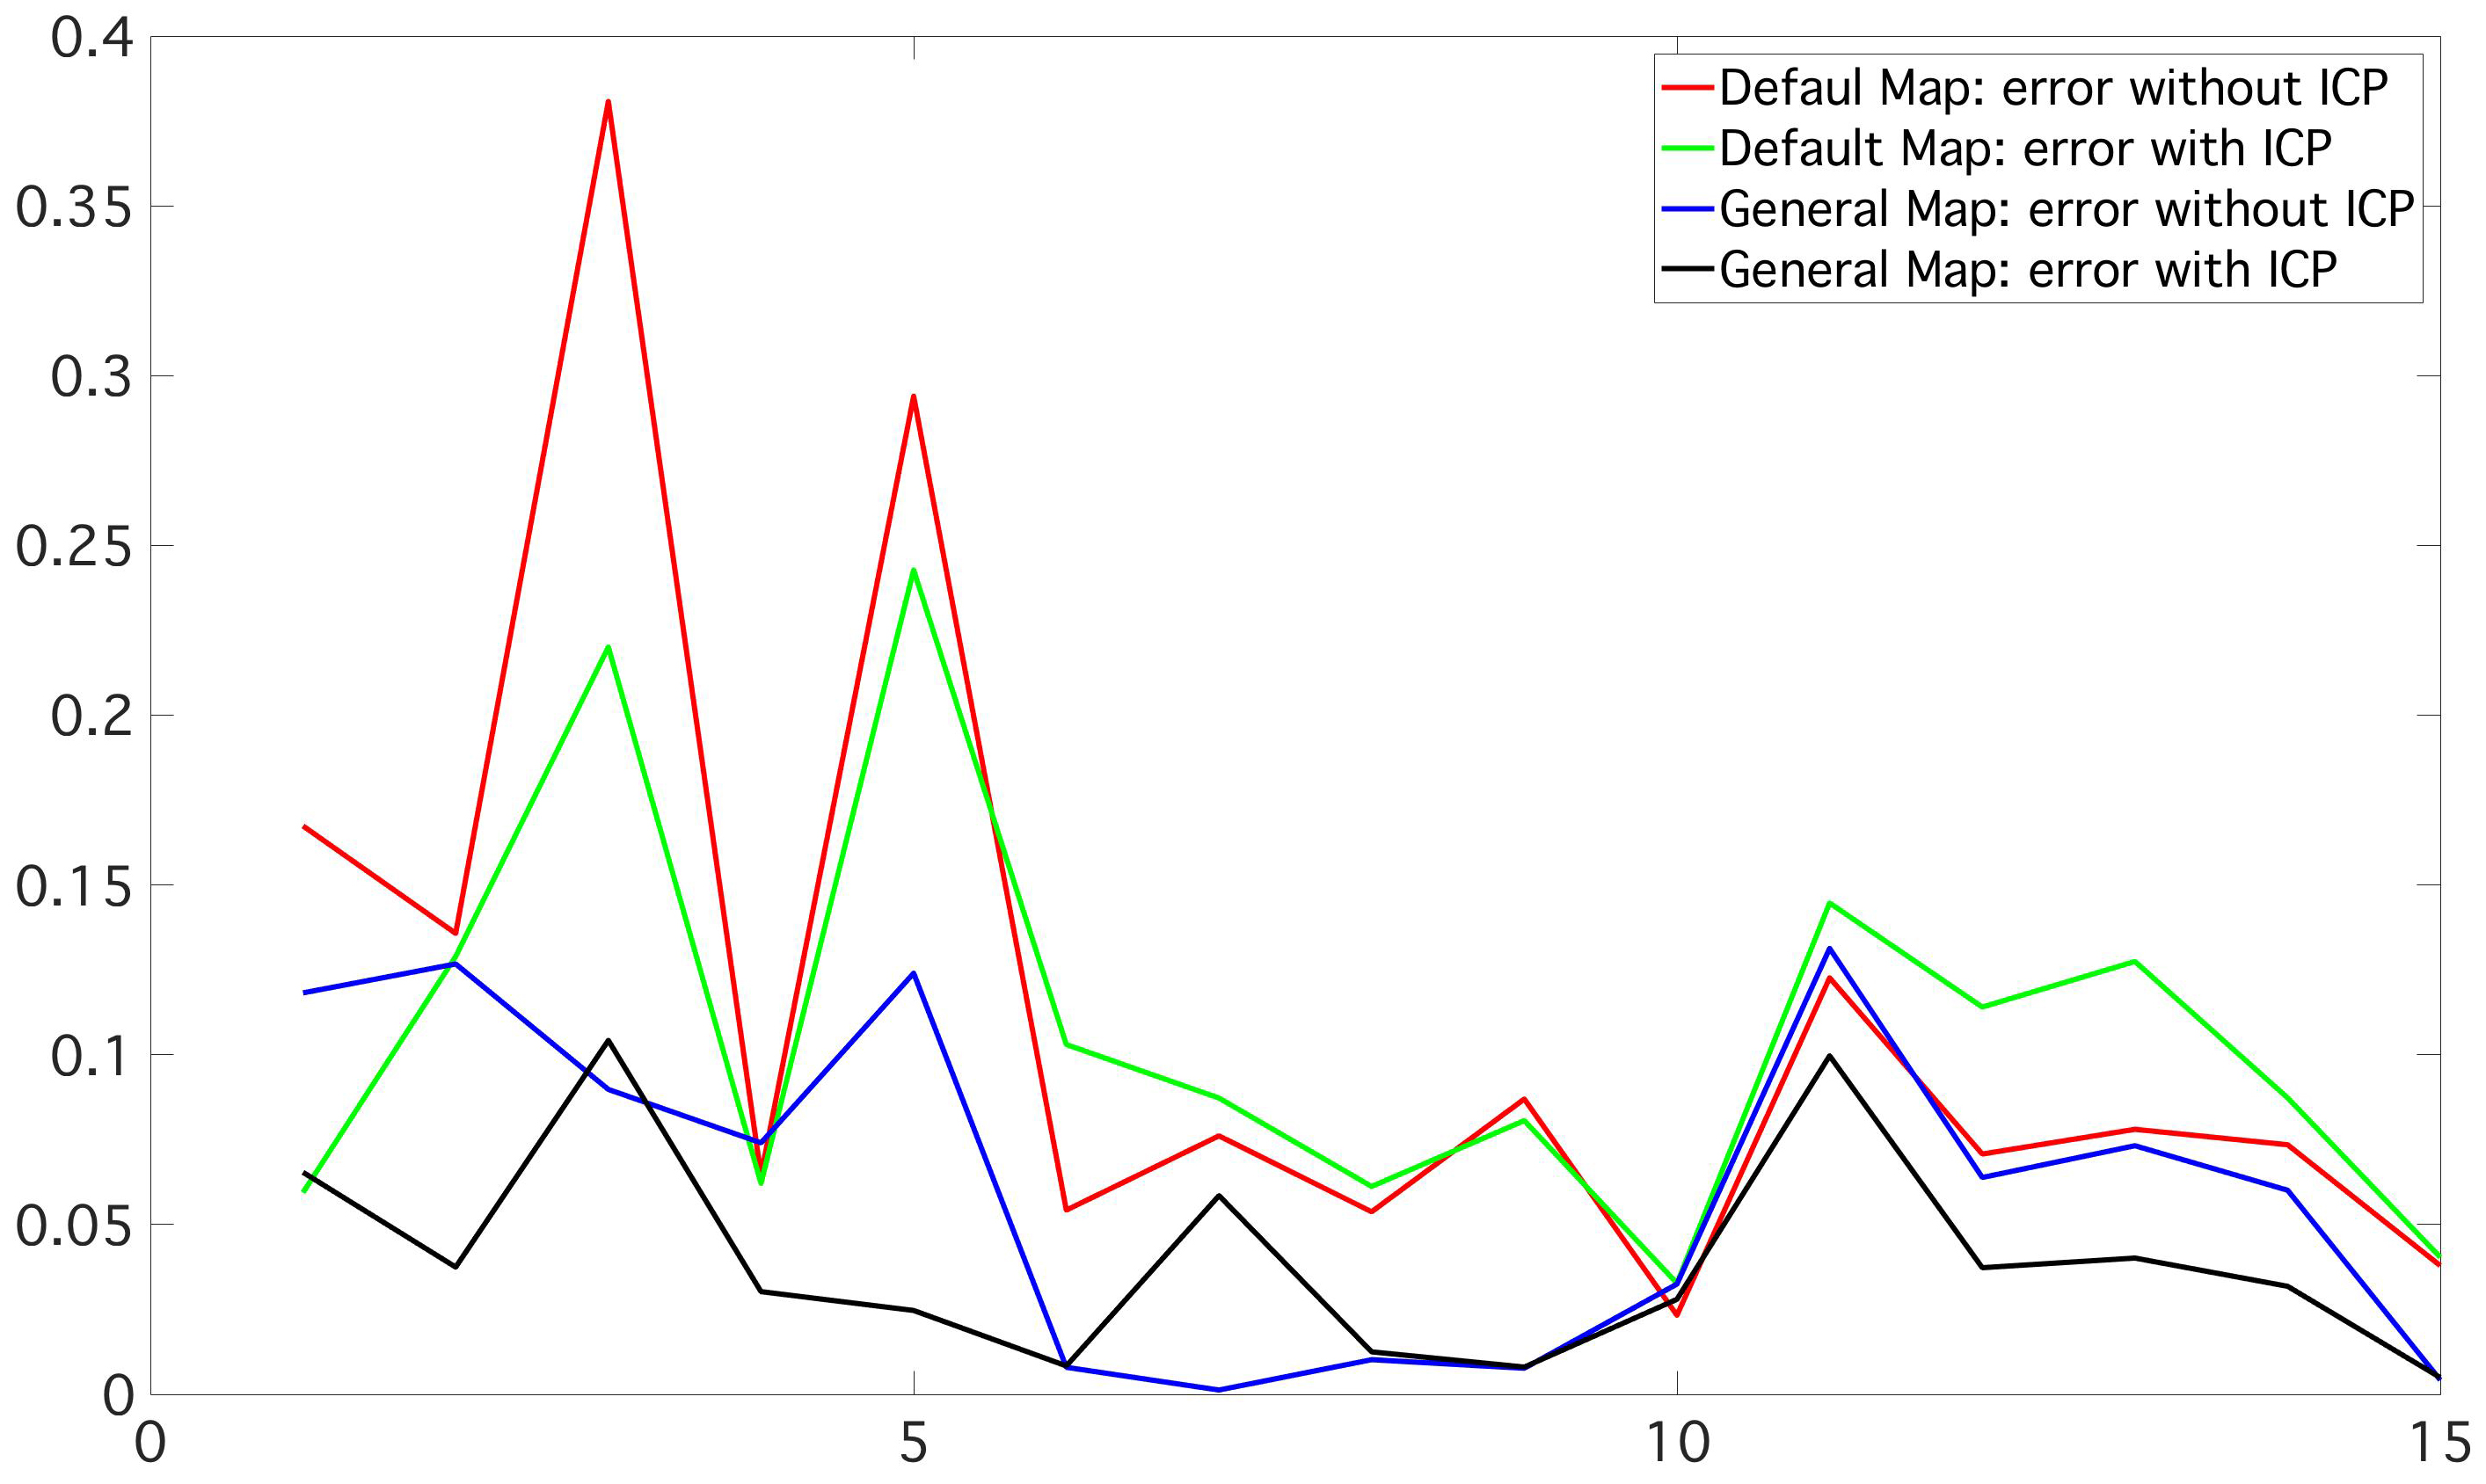
\includegraphics[height=105pt]{FMAP-images/bust-STATISTICS.jpg}
&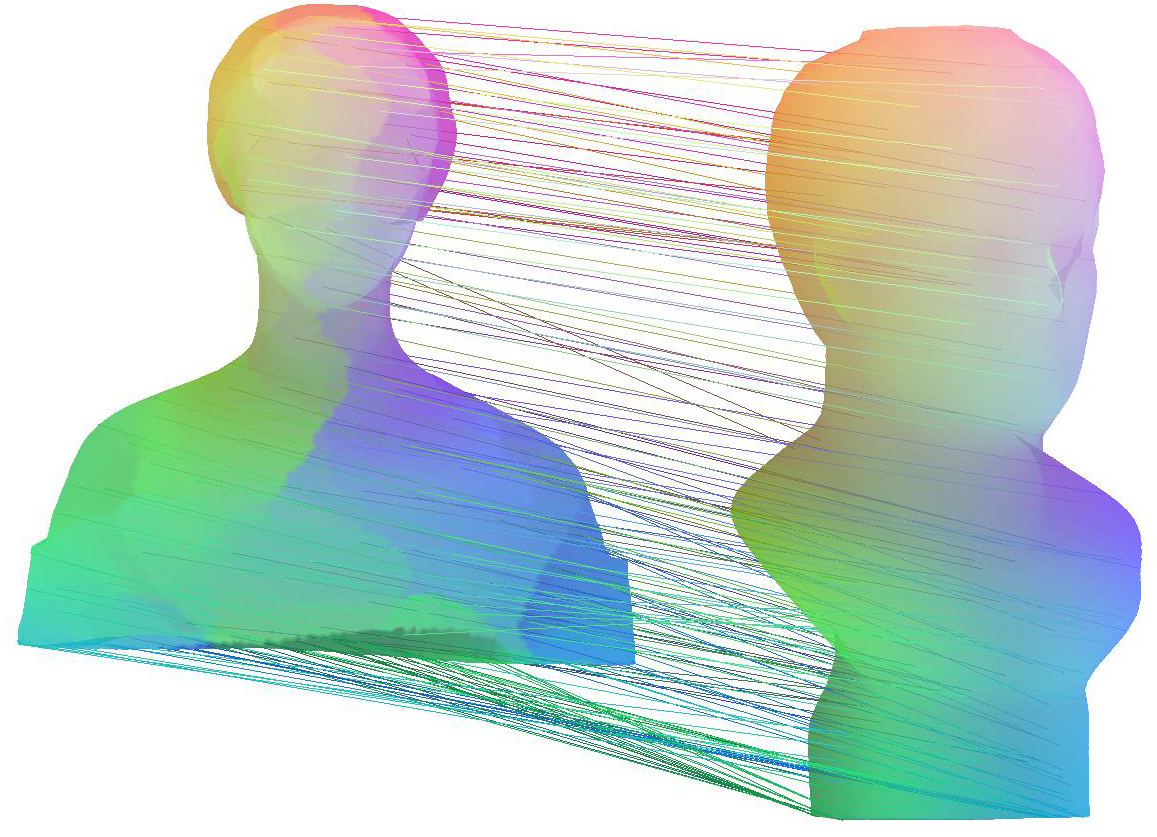
\includegraphics[height=85pt]{FMAP-images/bust-Source=301-Target=314-General-Basis-ZOOM.jpg}
&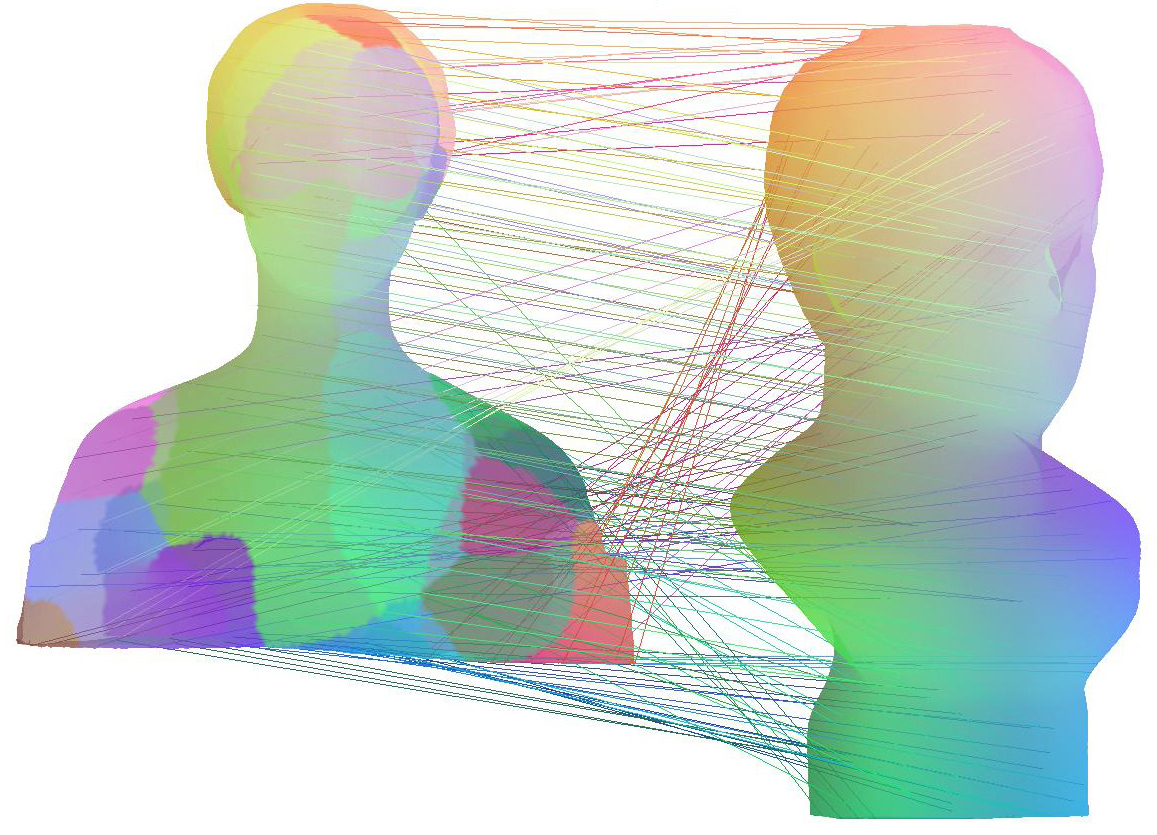
\includegraphics[height=85pt]{FMAP-images/bust-Source=301-Target=314-Lapl-Eig-ZOOM.jpg}\\
(d)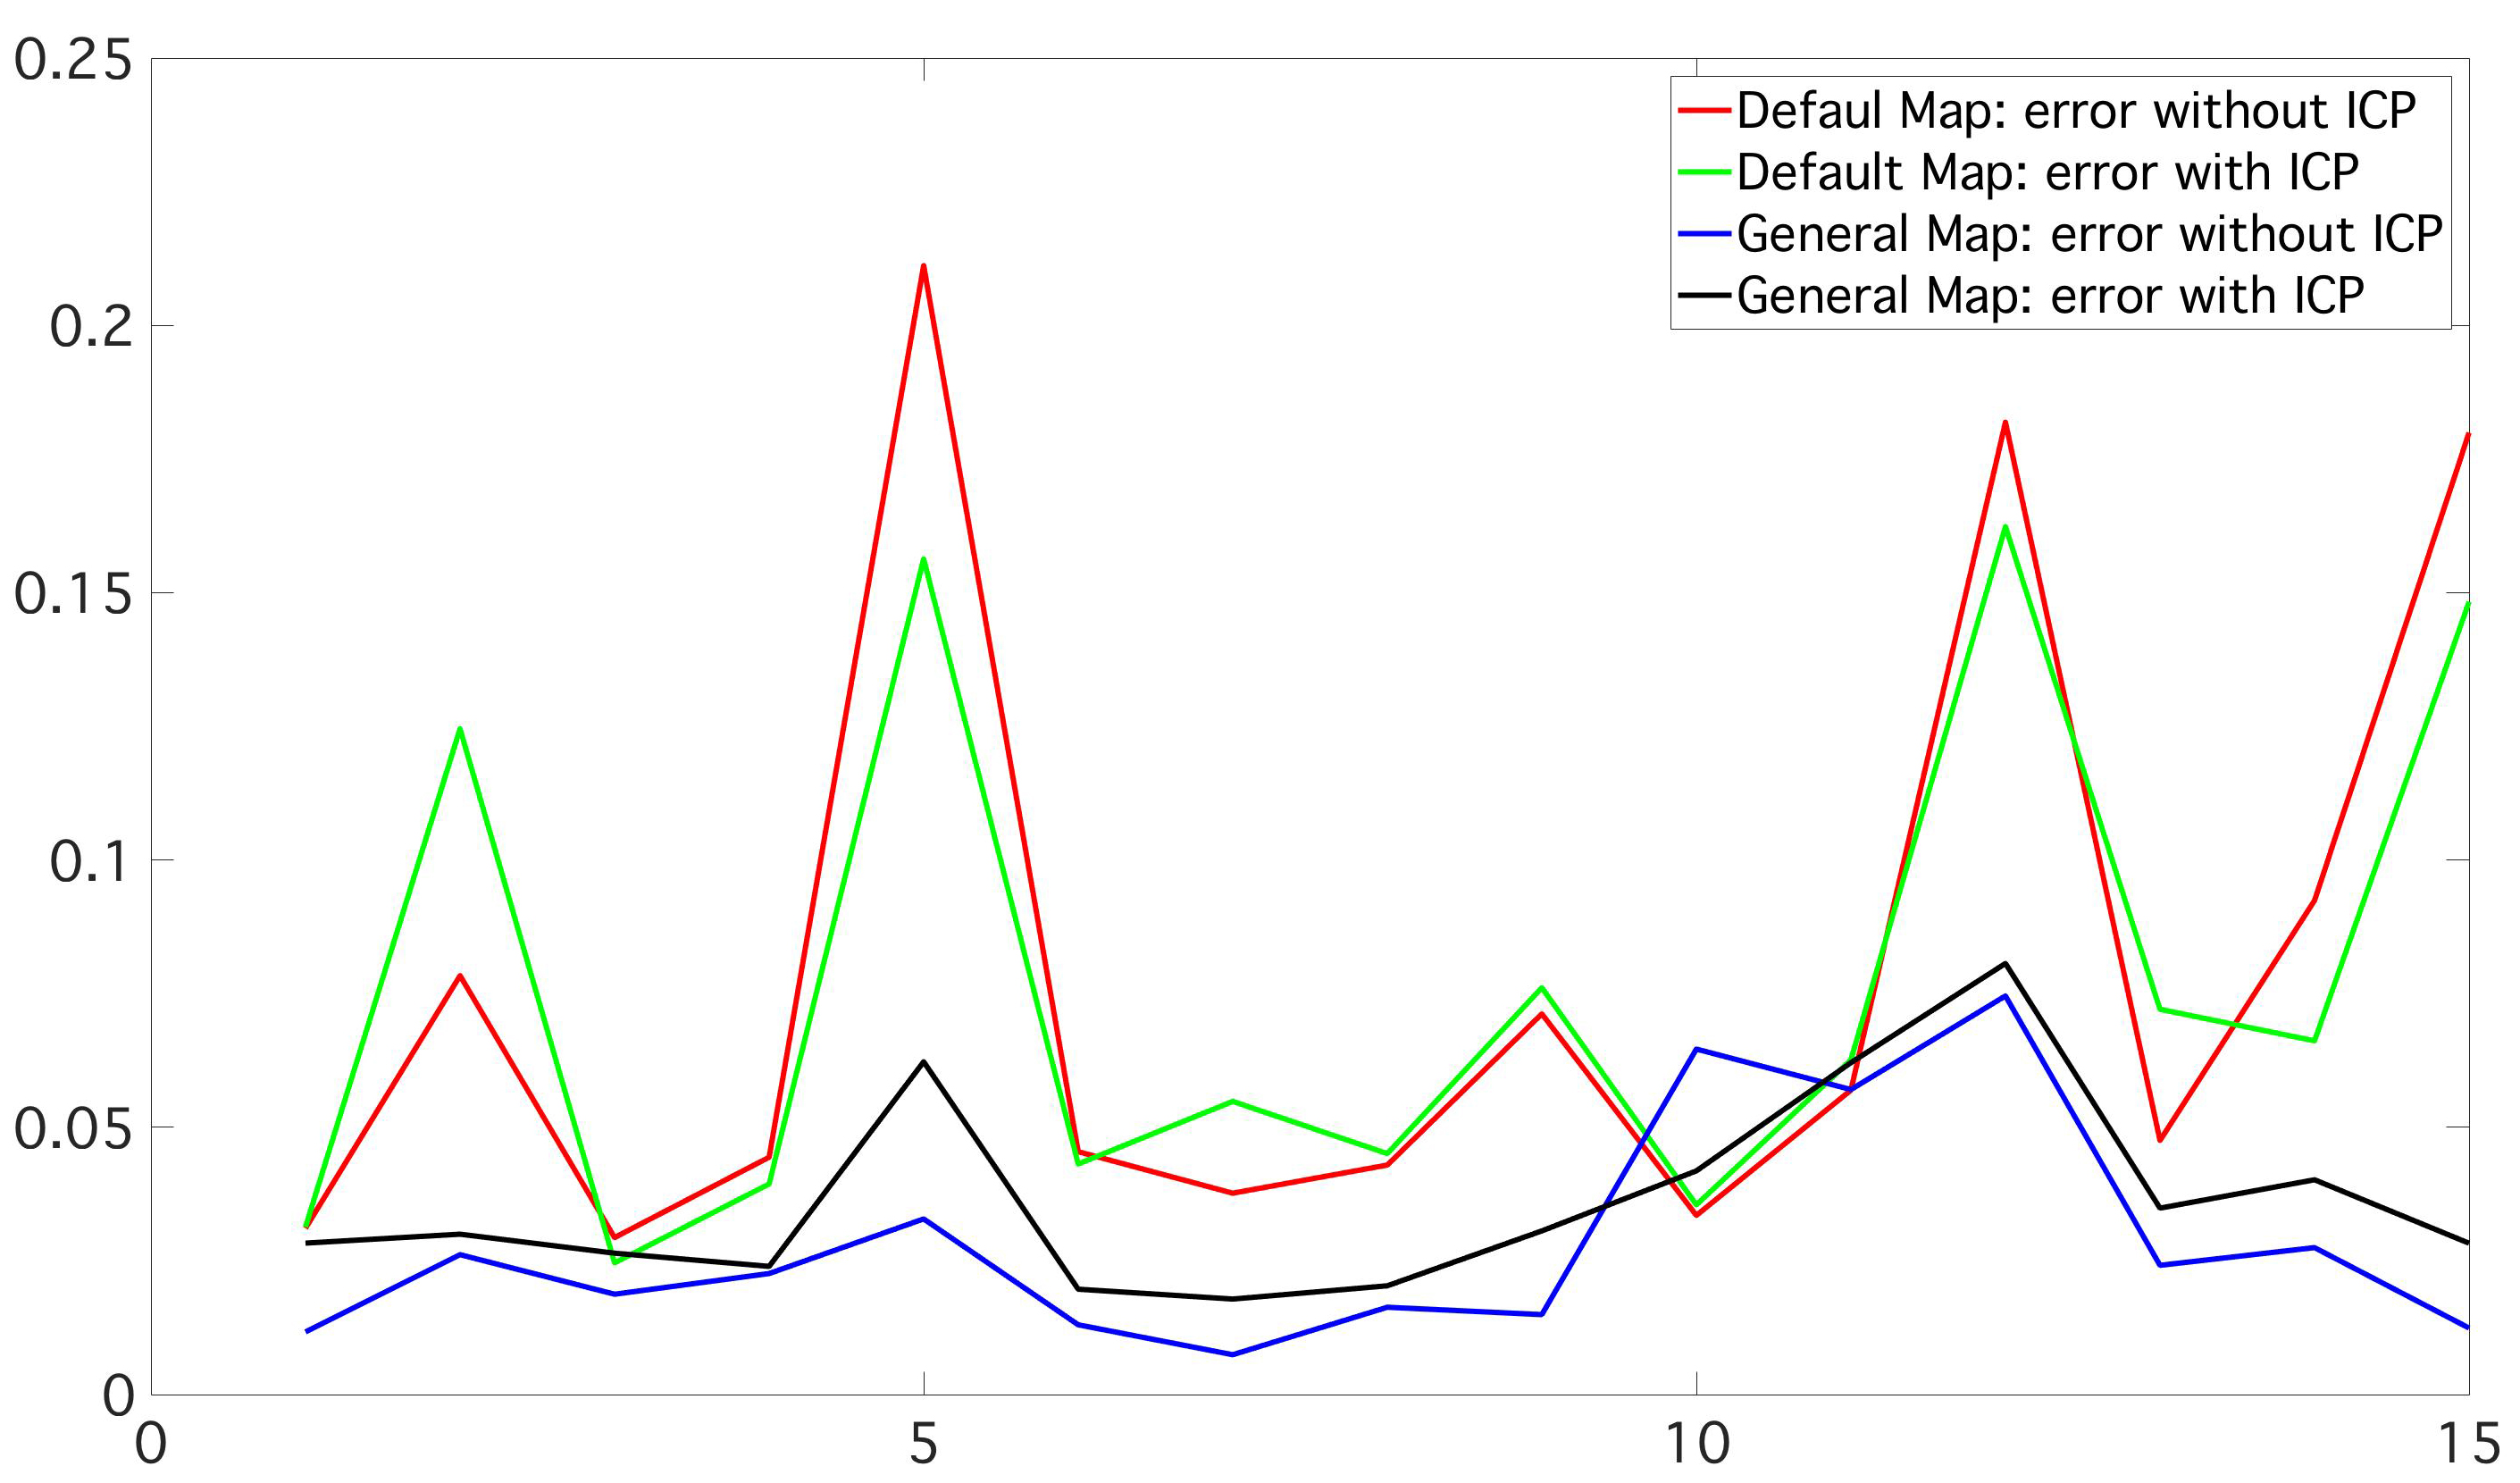
\includegraphics[height=105pt]{FMAP-images/human-STATISTICS.jpg}
&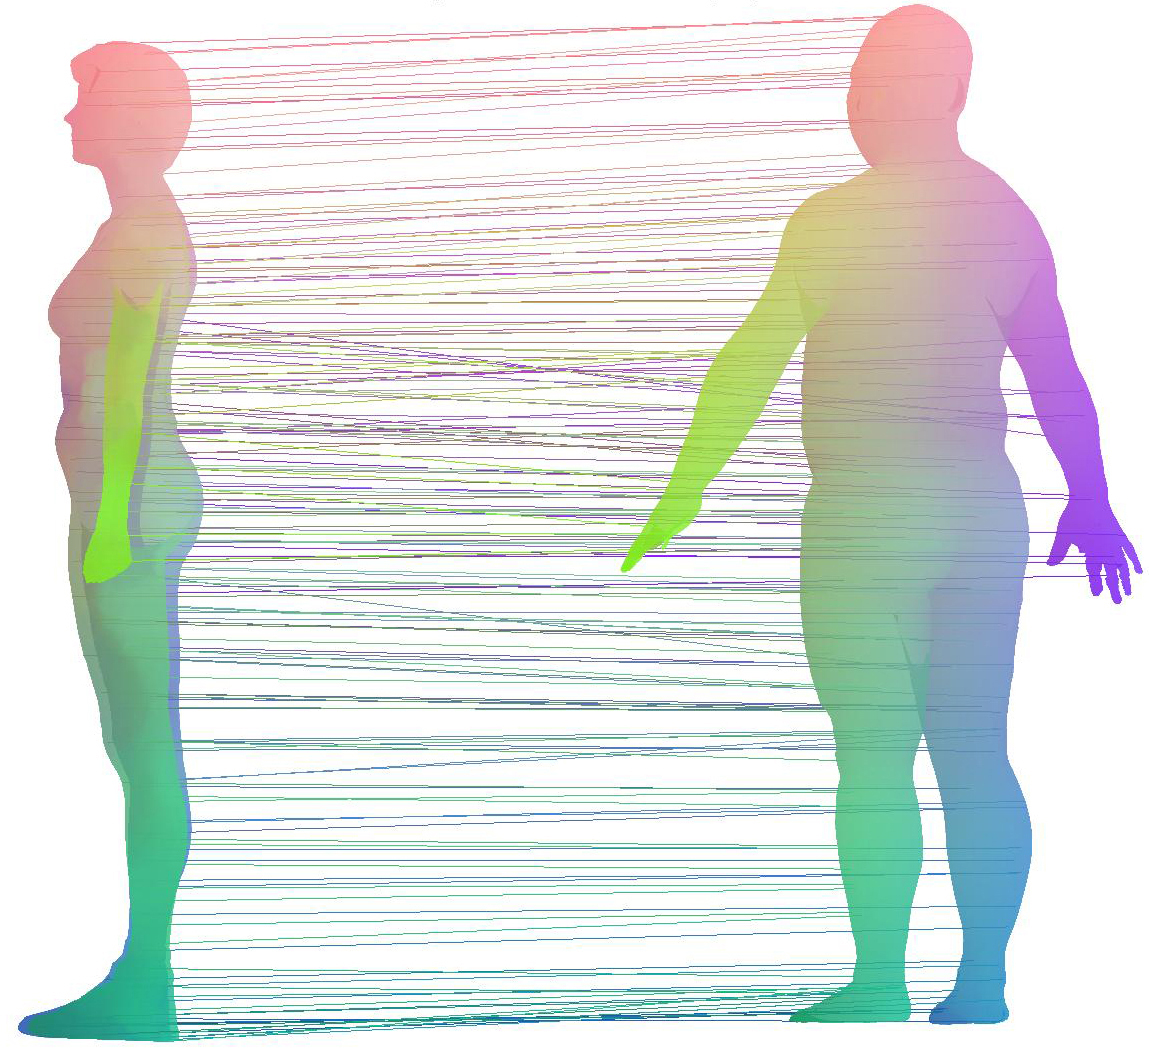
\includegraphics[height=85pt]{FMAP-images/human-Source=5-Target=10-General-Basis-ZOOM.jpg}
&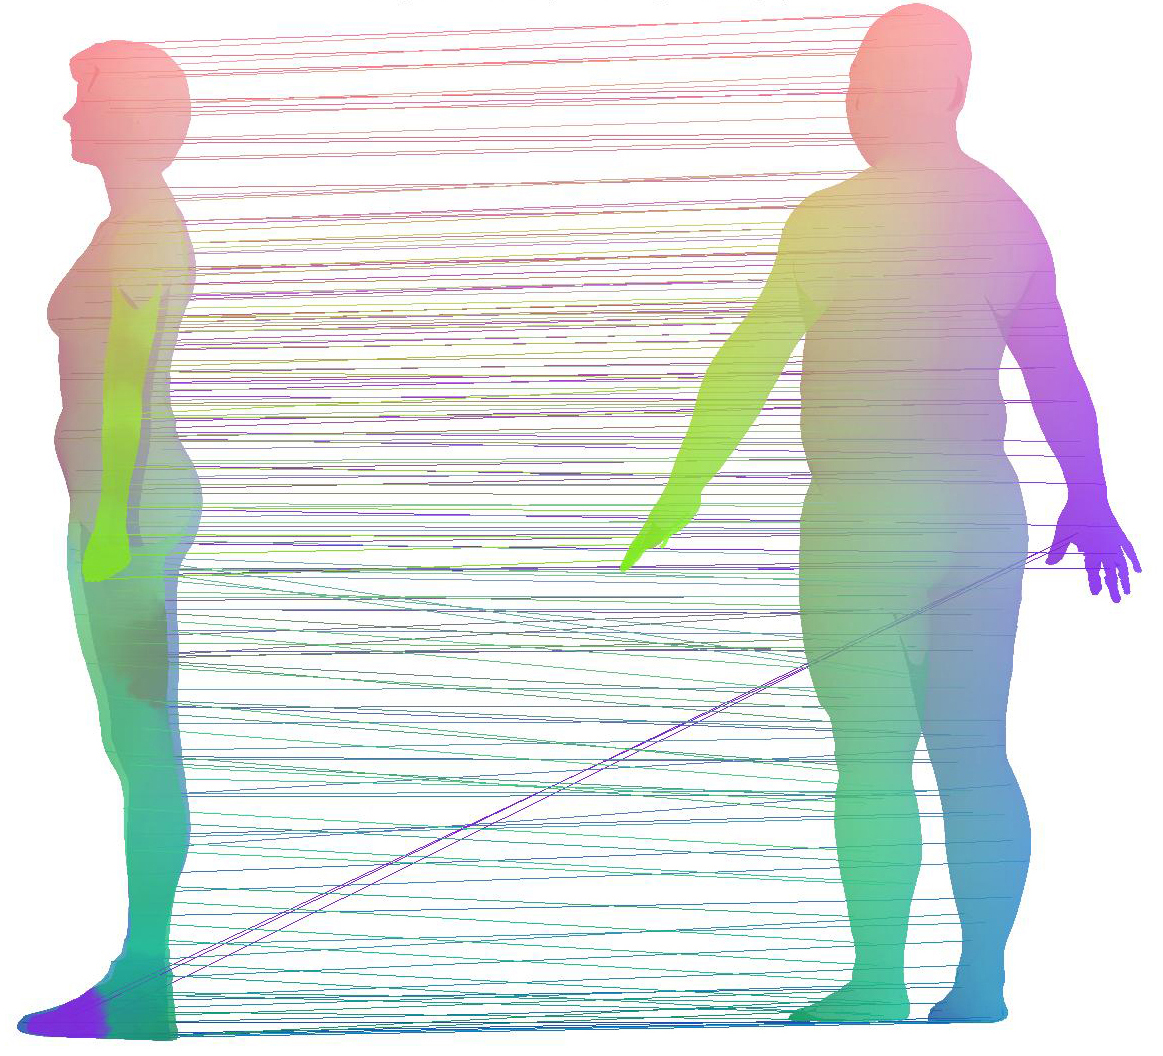
\includegraphics[height=85pt]{FMAP-images/human-Source=5-Target=10-Lapl-Eig-ZOOM.jpg}
\end{tabular}
\caption{Mean correspondence error ($y$-axis) on 15 couples ($x$-axis) of non-isometric SHREC shapes computed with the same number (i.e., \mbox{$k=60$}) of diffusion functions and Laplacian eigenfunctions. The diffusion functions generally provide a lower correspondence error before/after ICP and improve the quality of the correspondences; e.g., on (a) the plane wings, (b) the table legs, (c) the bottom and upper parts of the bust, (d) the legs and the harms.\label{fig:SHREC-DIFF-LAPL-SELECTION}}
\end{figure*}
%
\subsubsection{Orthonormalisation via QR factorisation\label{sec:QR-ORHTONORMALIZAION}}
Let~$\mathbf{Y}$ be the matrix whose columns are a set of the basis functions that are not orthogonal, or might be linearly dependent (e.g., a stack of different classes of basis functions). In these cases, the Gram-Schmidt and QR orthogonalisation~\citep{GOLUB1989} are used to replace the input functions with a set of orthonormal basis functions.

%Since the number of basis function is much smaller than the dimension~$n$ of the space of scalar functions defined on the input shape (here,~$n$ is the number of vertices), it is unlikely to deal with linearly independent basis functions. In fact, the probability that~$k$ basis functions are linearly dependent is~$k/n$. 

To extract a set of linearly independent and orthonormal basis functions from~$\mathbf{Y}$, we compute the QR factorisation~$\mathbf{Y}=\mathbf{Q}\mathbf{R}$ and select the first~$r$ linearly independent columns of~$\mathbf{Q}$, where~$r$ is the rank of~$\mathbf{Q}$. During the iteration of the QR factorisation, we impose that the columns of~$\mathbf{Q}$ are~$\mathbf{B}$-orthogonal (i.e., \mbox{$\mathbf{Q}^{\top}\mathbf{B}\mathbf{Q}=\mathbf{I}$}) instead of~$\ell_{2}$ orthogonal (i.e., \mbox{$\mathbf{Q}^{\top}\mathbf{Q}=\mathbf{I}$}). %Alternatively, we orthonormalise the selected~$r$ columns of~$\mathbf{Q}$ with the Gram-Schmidt method.
%
\begin{figure*}
\centering
\begin{tabular}{ccc}
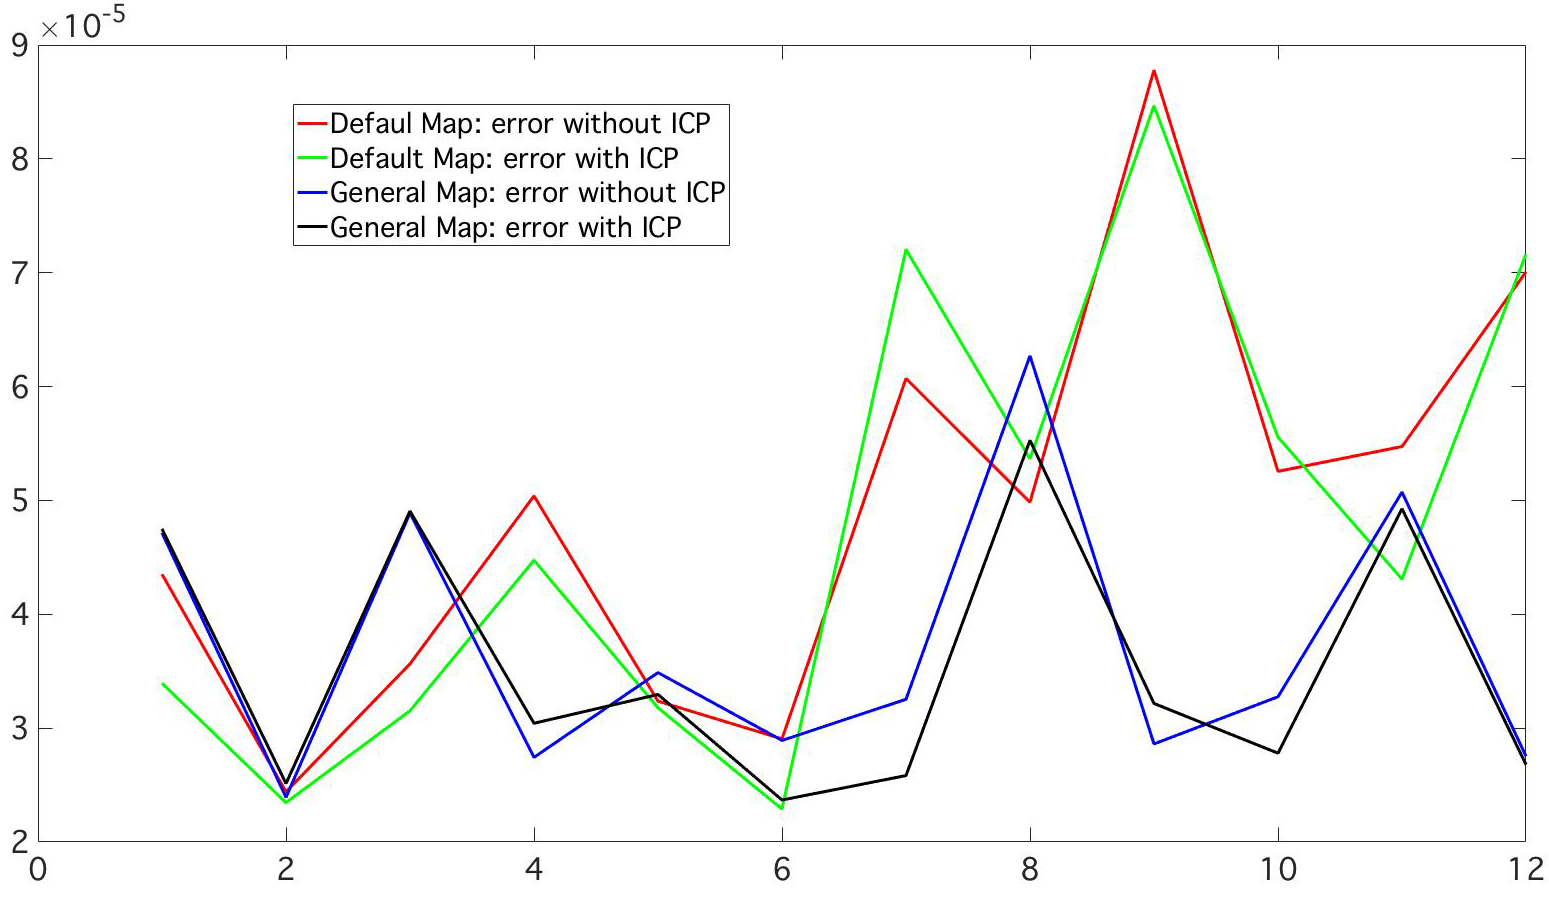
\includegraphics[height=110pt]{FMAP-images/data_man_woman_gorilla_matches-STATISTICS.jpg}
&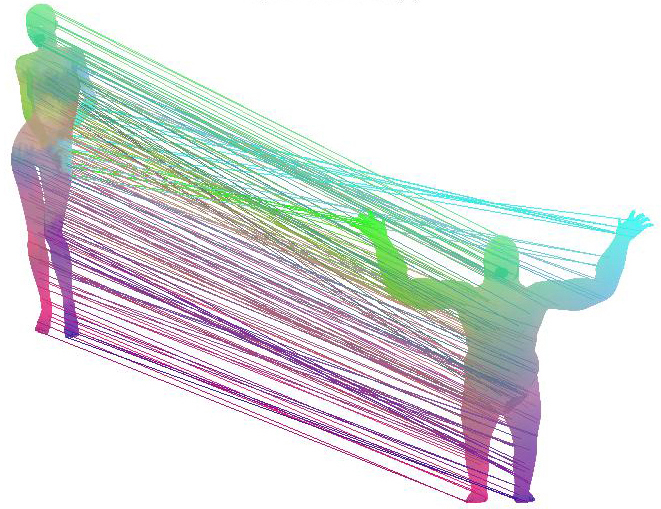
\includegraphics[height=110pt]{FMAP-images/data_man_woman_gorilla_matches-ZOOM-A.jpg}
&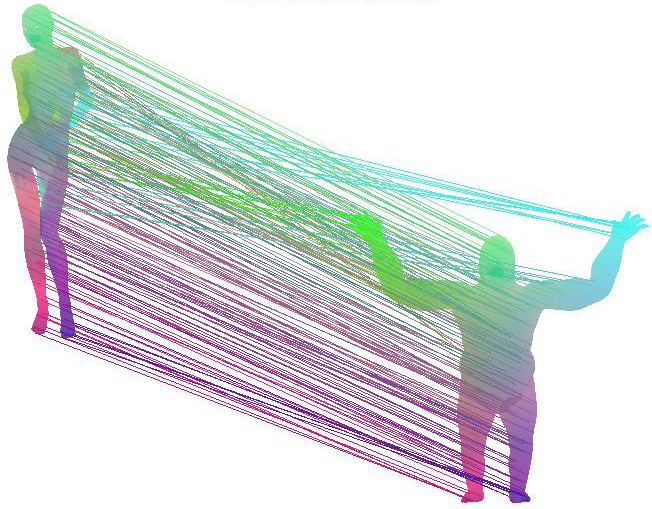
\includegraphics[height=110pt]{FMAP-images/data_man_woman_gorilla_matches-ZOOM-B.jpg}\\
(a) Mean correspondence error &(b)~$k=60$, Diffusion basis &(c)~$k=60$, Laplacian eigenbasis
\end{tabular}
\caption{(a,~$y$-axis) Mean correspondence error on 12 couples ($x$-axis) of non-isometric shapes of the TOSCA data set (c). With respect to the Laplacian eigenfunctions, the functional map induced by the diffusion basis (b) has a lower mean error and improves the quality of the correspondences on the right arm.\label{fig:TOSCA-CHALLENGE-MAN-GORILLA}}
\end{figure*}
%
\section{Discussion\label{sec:DISCUSSION}}
We now discuss the main properties of the harmonic and diffusion functions (Sect.~\ref{sec:BASIS-DISCUSSION}) and their application to the functional map framework (Sect.~\ref{sec:DISCUSSION-CORRESPONDENCE}).

\subsection{Basis functions: \label{sec:BASIS-DISCUSSION}}
%
\paragraph*{Harmonic basis}
According to our tests, the overall shape and distribution of the level-sets of the harmonic functions are preserved by the Gram-Schmidt orthonormalisation (Fig.~\ref{fig:MONKEY-HARM}).

\paragraph*{Diffusion basis}
In Fig.~\ref{fig:MONKEY-DIFFUSION}, the distribution of the level-sets of the input (first column) and orthonormalised (second column) diffusion functions at small scales (first two rows) shows the locality and multi-scale nature of the diffusion functions before and after orthonormalisation. At large scales (third row), the diffusion functions are no more centred at the seed points and have an analogous global behaviour; in fact, they tend to a constant function as the scale increases. Indeed, for the computation of shape correspondences we select small scales in order to have local diffusion functions.
 
For the analysis of the supports of the diffusion functions at small scales and their changes due to the orthonormalisation, we report the percentage of vertices belonging to the support of~$k$ input (Fig.~\ref{fig:SEEDS}a) and orthonormal (Fig.~\ref{fig:SEEDS}b) diffusion basis functions at 6 different scales \mbox{$(t=10^{-i})_{i=0}^{5}$}. These functions are centred at 50 seed points, which have been uniformly sampled on the input surface. At large scales (\mbox{$t=1$}, \mbox{$t=10^{-1}$}, respectively), the supports of a few (\mbox{$k\leq10$}) diffusion functions cover the whole surface. At tiny scales (\mbox{$t=10^{-5}$}, \mbox{$t=10^{-4}$}), the diffusion functions have no overlapping supports. 

The analogous behaviour of the curves in Fig.~\ref{fig:SEEDS} confirms that the Gram-Schmidt orthonormalisation generally does not increase the support of the diffusion functions at different scales (Fig.~\ref{fig:MONKEY-DIFFUSION}), as a matter of the ordering of the functions in the stack with respect to an increasing size of their support (i.e., from small to large scales), to the orthogonality of the diffusion functions with non-overlapping supports, and to a regular distribution of the seed points on the input surface through the farthest point sampling.

The set~$\mathcal{B}$ of diffusion basis functions at different scales and centred at different seed points might contain linearly dependent functions. If the number~$k$ of basis functions is much smaller than the dimension~$n$ of the space of scalar functions defined on the input shape (here,~$n$ is the number of vertices), then it is unlikely to deal with a large number of linearly dependent basis functions. In fact, the probability that~$k$ basis functions are linearly dependent is~$k/n$, which is generally low as \mbox{$k<<n$}. 

To study this aspect, we have analysed the rank of the matrix~$\mathbf{Y}$ whose columns are the functions in~$\mathcal{B}$, before and after the orhonormalisation. Our tests (Fig.~\ref{fig:MONKEY-DIFFUSION-RANK}a) show that~$\mathbf{Y}$ might be rank deficiency as a matter of small undulations of the input functions, to the analogous behaviour and locality (e.g., Fig.~\ref{fig:MONKEY-DIFFUSION}, 1st row; 1st, 2nd columns) of the diffusion functions centred at the same seed point and at different scales.

A similar discussion (Fig.~\ref{fig:MONKEY-DIFFUSION-RANK}b) also applies to the rank of a stack~$\mathcal{B}$ of harmonic, Laplacian, and diffusion basis functions. The linear independence of the orthonormalised functions confirms that the harmonic and diffusion functions at a relatively small set of seed points (with respect to the number of input vertices) and the Laplacian eigenfunctions encode different properties of the input shape. In case the low rank is not due to small undulations of the input functions but to a linear dependence of the input functions, then the QR factorisation of~$\mathbf{Y}$ is applied to remove the linearly dependent functions.
%
\begin{figure}[t]
\centering
Mean correspondence error\\
(a)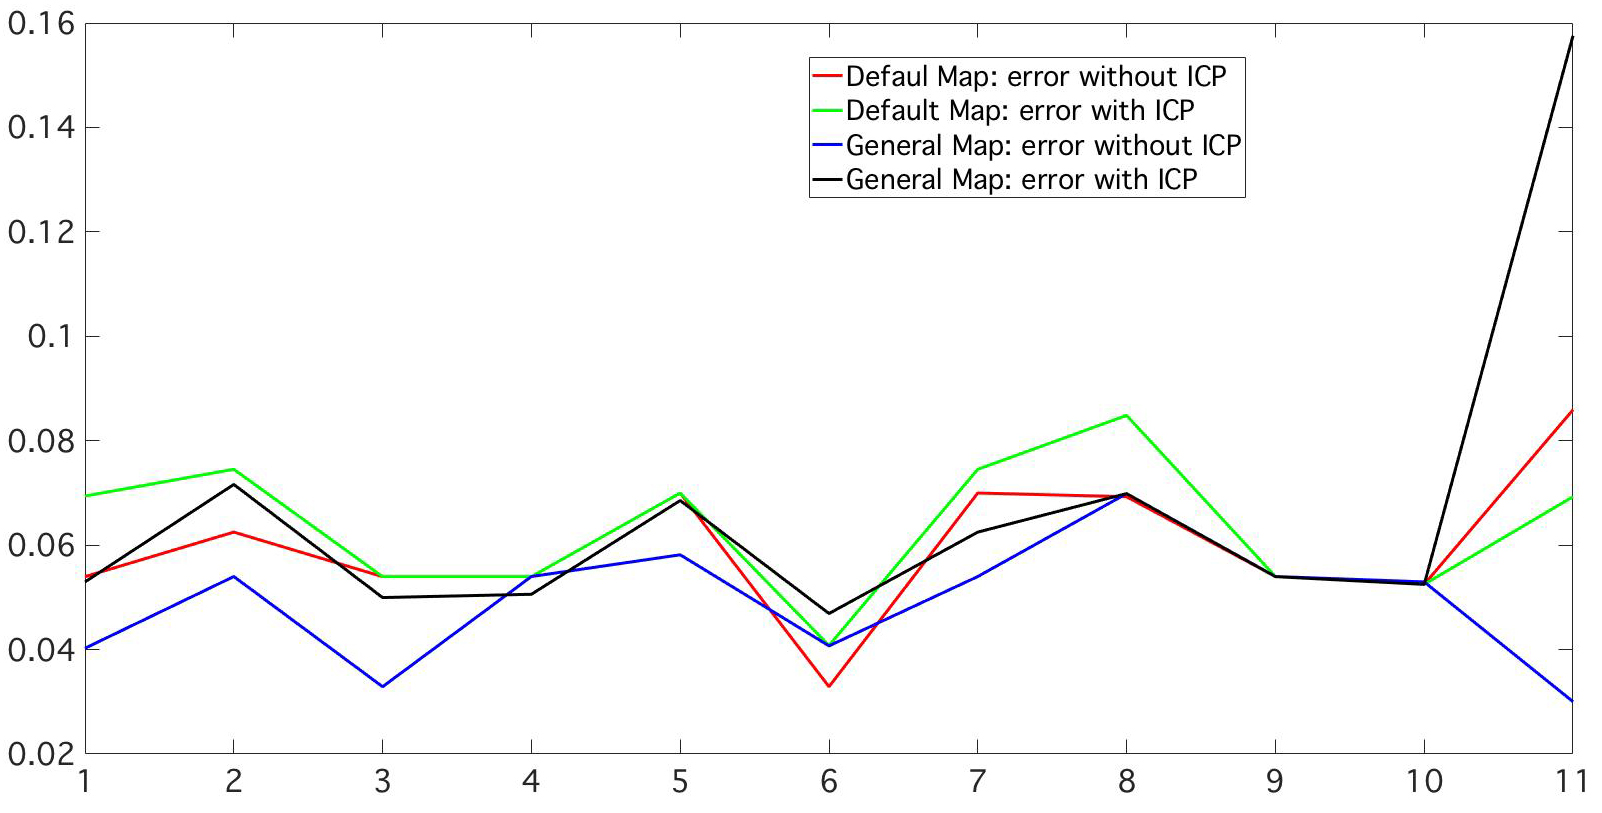
\includegraphics[height=100pt]{FMAP-images/victoria7-STATISTICS-2.jpg}
\begin{tabular}{c|c}
\hline
Harmonic basis &Laplacian eigenbasis\\
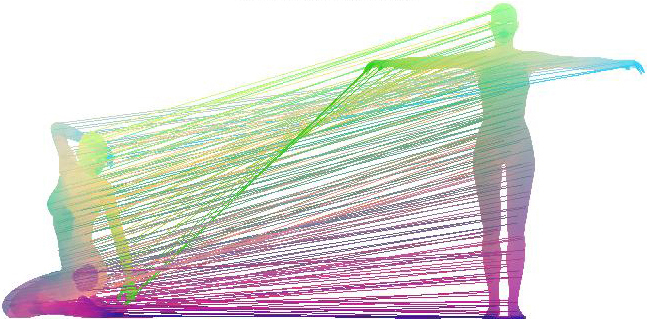
\includegraphics[width=140pt]{FMAP-images/Source=victoria0-Target=victoria23-General-Basis-ZOOM.jpg}
&\includegraphics[width=110pt]{FMAP-images/Source=victoria0-Target=victoria23-Lapl-Eig-ZOOM.jpg}\\
\includegraphics[width=110pt]{FMAP-images/Source=victoria0-Target=victoria24-General-Basis-ZOOM.jpg}
&\includegraphics[width=110pt]{FMAP-images/Source=victoria0-Target=victoria24-Lapl-Eig-ZOOM.jpg}\\
\includegraphics[width=110pt]{FMAP-images/Source=victoria0-Target=victoria25-General-Basis.jpg}
&\includegraphics[width=110pt]{FMAP-images/Source=victoria0-Target=victoria25-Lapl-Eig-ZOOM.jpg}\\
$k=60$ &$k=60$
\end{tabular}
\caption{(a,$y$-axis) Mean correspondence error on 11 couples (a,$x$-axis) of non-isometric shapes of the TOSCA data set. The harmonic basis slightly improves the correspondence error with respect to the the Laplacian eigenbasis (same number~$k$ of functions). The correspondences induced by both classes of basis functions have an analogous behaviour.\label{fig:VICTORI-CORRESPONDEMCE}}
\end{figure}
%
\subsection{Shape correspondences\label{sec:DISCUSSION-CORRESPONDENCE}}
For our experiments on shape correspondence, we select a low number~$k$ of ground-truth landmarks and consider the corresponding \mbox{$sk$} diffusion functions at~$s$ scales and/or the corresponding~$k$ harmonic functions. Indeed, the ground-truth landmarks are used to initialise the functional map and to define the functions that generate the sub-space on which the shape descriptors will be projected to define the functional map. To increase the initial number of basis functions, we can evaluate the diffusion/harmonic functions associated with an additional number of samples on the input shape. We compute these points with a farthest point sampling (e.g., from a given landmark or seed point) in order to have a uniform distribution on the input surface; alternatively, these additional seeds can be high-curvature or feature points.

For the examples of the paper, we usually select \mbox{$s=4$} small scales and \mbox{$2\leq k\leq 15$} ground-truth landmarks; however, these parameters can be tuned for each shape class, or according to the target storage/computational cost. For the computation of correspondences on almost isometric shapes, a low number of ground-truth landmarks (e.g., \mbox{$2\leq k\leq 5$}) is generally enough to disambiguate symmetric parts. For non-isometric shapes, we increase the number of ground-truth landmarks (e.g., \mbox{$7\leq k\leq 15$}) in order to improve the quality of the initialised functional map and to tailor the functional spaces on the source and target surfaces to these ground-truth correspondences, through a set of basis functions centred at these landmarks. In all the examples, the labels ``\emph{Default basis}'' and ``\emph{General basis}'' refer to the use of the Laplacian and the diffusion/harmonic functions for the computation of the functional map.
%
\begin{figure}[t]
\begin{tabular}{cc}
Harmonic basis &Laplacian basis\\
\hline
\includegraphics[width=90pt]{FMAP-images/TOSCA-10LANDMARKS-10LAPLACIAN-HARMONIC-BASIS-A.jpg}
&\includegraphics[width=90pt]{FMAP-images/TOSCA-10LANDMARKS-10LAPLACIAN-HARMONIC-BASIS-B.jpg}\\
10 Landmarks &\\
\hline
\includegraphics[width=90pt]{FMAP-images/TOSCA-10LANDMARKS-10LAPLACIAN-HARMONIC-BASIS-C.jpg}
&\includegraphics[width=90pt]{FMAP-images/TOSCA-10LANDMARKS-10LAPLACIAN-HARMONIC-BASIS-D.jpg}\\
15 Landmarks &\\
\hline
\includegraphics[width=90pt]{FMAP-images/TOSCA-10LANDMARKS-10LAPLACIAN-HARMONIC-BASIS-E.jpg}
&\includegraphics[width=90pt]{FMAP-images/TOSCA-10LANDMARKS-10LAPLACIAN-HARMONIC-BASIS-F.jpg}\\
20 Landmarks &\\
\hline
\end{tabular}
\caption{Shape correspondence computed with an increasing number~$k$ of ground-truth landmarks on the source and target non-isometric TOSCA shapes, and with~$k$ harmonic and Laplacian eigenfunctions. A larger number of landmarks corresponds to a larger number of harmonic basis functions centred at these points and to an improvement of the functional map (e.g., on the tail and legs). The correspondence induced by a low number (e.g., 10) of harmonic basis functions have some local inconsistencies, which are due to the highly non-isometric input shapes and disappear with a small increase of the ground-truth landmarks.\label{fig:ELEPHANT-HORSE}}
\end{figure}

In Fig.~\ref{fig:4LEGS-DIFFUSION-CORRESPONDENCES}(a, first row), we have selected 7 ground-truth landmarks, 5 uniformly sampled seed points and 4 scales on 15 shapes of the 4-legs class of the SHREC data set. The functional map induced by the corresponding 48 diffusion functions has been compared with the one induced by 60 Laplacian eigenfunctions. According to the variation of the mean correspondence error in (a) and the examples of correspondences in the first and second rows, the diffusion basis functions generally provide a lower correspondence error before and after the optimisation based on the Iterative Closed Point (ICP, for short)~\citep{NOGNENG2017}. Furthermore, the diffusion functions improve the quality of the correspondences with respect to the Laplacian eigenbasis; e.g., between (left) the legs of the giraffe and the tail of the cow, (middle) the legs of the giraffe and the horns of the goat, (right) the legs of the dog and the horns of the cow. Finally, a small increase of the number of landmarks (Fig.~\ref{fig:4LEGS-DIFFUSION-CORRESPONDENCES}b, from 7 to 10 landmarks) reduces the mean correspondence error approximately of the \mbox{$50\%$}. The improvement of these results is also due to the multi-scale nature of the diffusion functions at the same seed points, which have been uniformly sampled on the input surface.

A similar discussion applies to the examples in Fig.~\ref{fig:SHREC-DIFF-LAPL-SELECTION}, where we have computed the correspondences between 15 couples of shapes belonging to 4 classes of the SHREC data set. Here, we have considered the same number (i.e., \mbox{$k=60$}) of diffusion functions (i.e., 15 seed points, 4 scales) and Laplacian eigenfunctions. For the rigid and articulated shapes, the correspondence error is always lower than 0.15 and the computed correspondences correctly map local and global features on the source and target shape.

Our experiments on non-isometric shapes of the TOSCA data set confirm that the functional map induced by the diffusion (Fig.~\ref{fig:TOSCA-CHALLENGE-MAN-GORILLA}) or harmonic (Fig.~\ref{fig:VICTORI-CORRESPONDEMCE}) functions generally has a lower mean error with respect to the Laplacian eigenfunctions. This smaller error (Fig.~\ref{fig:TOSCA-CHALLENGE-MAN-GORILLA}a) is also reflected in the quality of the computed correspondences (Fig.~\ref{fig:TOSCA-CHALLENGE-MAN-GORILLA}b). In Fig.~\ref{fig:VICTORI-CORRESPONDEMCE}, the behaviour of the correspondences induced by the harmonic functions and the Laplacian eigenfunctions is quite similar.

In Fig.~\ref{fig:ELEPHANT-HORSE}, we have computed the shape correspondences with an increasing number~$k$ of ground-truth landmarks on the source and target non-isometric TOSCA shapes, and with~$k$ harmonic and Laplacian eigenfunctions. A larger number of landmarks corresponds to a larger number of harmonic basis functions centred at these points and to an improvement of the functional map (e.g., on the tail and legs). Since the Laplacian basis functions are independent of the selected landmarks, a larger number of landmarks only improves the quality of the descriptor used to initialise the functional map and does not significantly improve the underlying functional map and the resulting correspondences. The correspondences induced by a low number (e.g., 10) of harmonic basis functions have some local inconsistencies that are due to the highly non-isometric input shapes; however, these local artefacts disappear with a low increase of the ground-truth landmarks. 

Finally, the examples of Fig.~\ref{fig:SHREC-STATISTICS} the diffusion functions generally provide the lowest mean correspondence error with respect to the Laplacian eigenfunctions.

\section{Conclusions and future work}\label{sec:CONCLUSION}
In this paper, we have proposed a new way to define a set of basis functions that are informative, orthonormal, multi-scale, shape-aware, centred/localised, easily computable, and isometry-invariant.

Our experiments on the non-isometric SHREC (Fig.~\ref{fig:4LEGS-DIFFUSION-CORRESPONDENCES}, Fig.~\ref{fig:SHREC-DIFF-LAPL-SELECTION}, Fig.~\ref{fig:SHREC-STATISTICS}) and on the TOSCA (Fig.~\ref{fig:TOSCA-CHALLENGE-MAN-GORILLA}, Fig.~\ref{fig:VICTORI-CORRESPONDEMCE}, Fig.~\ref{fig:ELEPHANT-HORSE}) data sets show the improvement of the proposed basis functions on the the computation of shape correspondences through the functional map framework with respect to the Laplacian eigenbasis. This improvement is related mainly to the reduction of the mean correspondence error and better correspondences between the source and target shapes. The proposed basis functions also allow us to adapt their number and behaviour to the local shape geometry, through the selection of their seed points and locality (i.e., support size), to the number of input ground-truth landmarks, and to the complexity of the input surface and its underlying functional space.

For the computation of the functional map, it is generally useful to center the harmonic and diffusion functions at ground-truth landmarks and at uniformly sampled points in order to encode a sufficient set of local geometric features in the corresponding basis functions, as these features will be also encoded by the shape descriptors used to initialise the functional map. Furthermore, uniformly sampled seeds provide a simple way to guarantee the shape coverage by the supports of the locally-supported diffusion functions.

As future work, we mention the optimal selection of the seed points with respect to the minimisation of the mean correspondence error and the identification of the best correspondences between the source and target shapes. To this end, we plan to use the proposed approach as initial step of an iterative procedure that updates the position of coupled seeds according to the reduction, and possibly minimisation, of the mean correspondence error. Another aspect is the definition of new classes of basis functions as solutions to other differential equations (e.g., induced by the Hamiltonian, Steklov operators~\citep{CHOUKROUN-CORR2017,WANG2018}) associated with the Laplace-Beltrami operator.
%
\bibliographystyle{ACM-Reference-Format}
%\bibliographystyle{ACM-Reference-Format-Journals}
\bibliography{FMAP-BIBLIOGRAPHY}
%
\newpage
%
\begin{figure*}
\centering
\begin{tabular}{cc||cc}
\multicolumn{2}{c||}{\textbf{$40$ Diffusion~$\&$ Laplacian functions;~$40\%$ Ground-truth Land.}}
&\multicolumn{2}{|c}{\textbf{$60$ Diffusion~$\&$ Laplacian functions;~$50\%$ Ground-truth Land.}}\\
\hline
Human &Cup &Human &Cup\\
\includegraphics[width=120pt]{FMAP-images/1-STATISTICS-40.jpg} 		%Human
&\includegraphics[width=120pt]{FMAP-images/2-STATISTICS-40.jpg} 	%Cup
&\includegraphics[width=120pt]{FMAP-images/1-STATISTICS-50.jpg} 	%Human
&\includegraphics[width=120pt]{FMAP-images/2-STATISTICS-50.jpg}\\	%Cup
\hline
%\includegraphics[width=110pt]{FMAP-images/3-STATISTICS-40.jpg} 	%Glsses
%&\includegraphics[width=110pt]{FMAP-images/4-STATISTICS-40.jpg} 	%Plane
%&\includegraphics[width=110pt]{FMAP-images/3-STATISTICS-50.jpg}	 %Glaases
%&\includegraphics[width=110pt]{FMAP-images/4-STATISTICS-50.jpg}\\	%Plane
%\includegraphics[width=110pt]{FMAP-images/5-STATISTICS-40.jpg} 	%Ant
%&\includegraphics[width=110pt]{FMAP-images/5-STATISTICS-50.jpg} 	%Ant
Octopus &Table &Octopus &Table\\
\includegraphics[width=120pt]{FMAP-images/7-STATISTICS-40.jpg} 		%Octupua
&\includegraphics[width=120pt]{FMAP-images/8-STATISTICS-40.jpg} 	%Table
&\includegraphics[width=120pt]{FMAP-images/7-STATISTICS-50.jpg}		%Octupus
&\includegraphics[width=120pt]{FMAP-images/8-STATISTICS-50.jpg}\\	%Table
\hline
Teddy &Hand &Teddy &Hand\\
\includegraphics[width=120pt]{FMAP-images/9-STATISTICS-40.jpg}		%Teddy
&\includegraphics[width=120pt]{FMAP-images/10-STATISTICS-40.jpg}	%Hand	
&\includegraphics[width=120pt]{FMAP-images/9-STATISTICS-50.jpg}		%Teddy
&\includegraphics[width=120pt]{FMAP-images/10-STATISTICS-50.jpg}\\	%Hand
\hline
%\includegraphics[width=110pt]{FMAP-images/11-STATISTICS-40.jpg}	%Piler
%&\includegraphics[width=110pt]{FMAP-images/12-STATISTICS-40.jpg}	%Fish
%&\includegraphics[width=110pt]{FMAP-images/11-STATISTICS-50.jpg}	%Piler
%&\includegraphics[width=110pt]{FMAP-images/12-STATISTICS-50.jpg}\\	%Fish
%\includegraphics[width=110pt]{FMAP-images/13-STATISTICS-40.jpg}	%Bird	
%&\includegraphics[width=110pt]{FMAP-images/14-STATISTICS-40.jpg}	%Sping
%&\includegraphics[width=110pt]{FMAP-images/13-STATISTICS-50.jpg}	%Bird
%&\includegraphics[width=110pt]{FMAP-images/14-STATISTICS-50.jpg}\\	%Spring
Armadillo &Bust &Armadillo &Bust\\
\includegraphics[width=120pt]{FMAP-images/15-STATISTICS-40.jpg}		%Armadillo
&\includegraphics[width=120pt]{FMAP-images/16-STATISTICS-40.jpg}	%Bust
&\includegraphics[width=120pt]{FMAP-images/15-STATISTICS-50.jpg}	%Armadillo
&\includegraphics[width=120pt]{FMAP-images/16-STATISTICS-50.jpg}\\	%Bust
\hline
Mech &Bearing &Mech &Bearing\\
\includegraphics[width=120pt]{FMAP-images/17-STATISTICS-40.jpg}		%Mech
&\includegraphics[width=120pt]{FMAP-images/18-STATISTICS-40.jpg}	%Bearing
&\includegraphics[width=120pt]{FMAP-images/17-STATISTICS-40.jpg}	%Mech
&\includegraphics[width=120pt]{FMAP-images/18-STATISTICS-50.jpg}\\	%Bearing
\hline
Chair &Fourlegs &Chair &Fourlegs\\
\includegraphics[width=120pt]{FMAP-images/6-STATISTICS-40.jpg}		%Chair
&\includegraphics[width=120pt]{FMAP-images/19-STATISTICS-40.jpg}	%Fourleg
&\includegraphics[width=120pt]{FMAP-images/6-STATISTICS-50.jpg}		%Chair
&\includegraphics[width=120pt]{FMAP-images/19-STATISTICS-50.jpg}	%Fourleg
\end{tabular}
\caption{Variation of the mean correspondence errors within 10 (most challenging) classes of the SHREC data set, computed with~$k$ diffusion and Laplacian functions, and a different percentage (i.e.,~$40\%$,~$50\%$) of selected ground-truth landmarks. The randomly selected ground-truth landmarks are also used to initialise the functional map framework and as seed points of the diffusion functions at 4 scales, together with an additional number~$a$ of uniformly sampled seed points. The value~$a$ depends on~$s$ and~$k$; for \mbox{$k=40, 60$} diffusion functions, \mbox{$a=(10-s)$} and \mbox{$a=(15-s)$}, respectively. In all the examples, the diffusion functions generally provide the lowest mean correspondence error with respect to the Laplacian eigenfunctions.\label{fig:SHREC-STATISTICS}}
\end{figure*}
%
\end{document}